\documentclass[a4paper,11pt,fleqn,dvipsnames,oneside,openright]{memoir} 	% Openright aabner kapitler paa hoejresider (openany begge)

%%%% PACKAGES %%%%

% ¤¤ Oversaettelse og tegnsaetning ¤¤ %
\usepackage[utf8]{inputenc}					% Input-indkodning af tegnsaet (UTF8)
\usepackage[danish]{babel}					% Dokumentets sprog
\usepackage[T1]{fontenc}					% Output-indkodning af tegnsaet (T1)
\usepackage{ragged2e,anyfontsize}			% Justering af elementer
\usepackage{fixltx2e}						% Retter forskellige fejl i LaTeX-kernen
																			
% ¤¤ Figurer og tabeller (floats) ¤¤ %
\usepackage{graphicx} 						% Haandtering af eksterne billeder (JPG, PNG, EPS, PDF)

\usepackage{subfig}

%\usepackage{eso-pic}						% Tilfoej billedekommandoer paa hver side
%\usepackage{wrapfig}						% Indsaettelse af figurer omsvoebt af tekst. \begin{wrapfigure}{Placering}{Stoerrelse}
\usepackage[space]{grffile}					% Bør gøre det muligt at have mellemrum i filnavne.
\usepackage{multirow}                		% Fletning af raekker og kolonner (\multicolumn og \multirow)
\usepackage{multicol}         	        	% Muliggoer output i spalter
\usepackage{rotating}						% Rotation af tekst med \begin{sideways}...\end{sideways}
\usepackage{colortbl} 						% Farver i tabeller (fx \columncolor og \rowcolor)
\usepackage[usenames,dvipsnames]{xcolor}	% Definer farver med \definecolor. Se mere: http://en.wikibooks.org/wiki/LaTeX/Colors
%\usepackage{flafter}						% Soerger for at floats ikke optraeder i teksten foer deres reference
\let\newfloat\relax 						% Justering mellem float-pakken og memoir
\usepackage{float}							% Muliggoer eksakt placering af floats, f.eks. \begin{figure}[H]
\setlength{\heavyrulewidth}{0.15em}			% Sætter \toprule og \bottomrule til fast størrelse (0.08 er default)
%\setlength{\lightrulewidth}{0.05em}		% Sætter \midrule til fast størrelse (0.05 er default)
\usepackage{array}							% Bruges i forbindelse med \newcolumntype-command under egne commands
\usepackage{pdfpages}						% Bruges så der kan indsættes pdf, som sider (forside for eksempel)
\usepackage{wrapfig}
\usepackage[section]{placeins}				% Indsætter en border så billeder bliver placeret inden for den section de er indsat
\usepackage{lastpage}						% Anvendes til at se total antal sider

% ¤¤ Matematik mm. ¤¤
\usepackage{amsmath,amssymb,stmaryrd} 		% Avancerede matematik-udvidelser
\usepackage{mathtools}						% Andre matematik- og tegnudvidelser
\usepackage{textcomp}                 		% Symbol-udvidelser (f.eks. promille-tegn med \textperthousand )
\usepackage{rsphrase}						% Kemi-pakke til RS-saetninger, f.eks. \rsphrase{R1}
\usepackage[version=3]{mhchem} 				% Kemi-pakke til flot og let notation af formler, f.eks. \ce{Fe2O3}
\usepackage{siunitx}						% Flot og konsistent praesentation af tal og enheder med \si{enhed} og \SI{tal}{enhed}
\sisetup{locale=DE}							% Opsaetning af \SI (DE for komma som decimalseparator) 

% ¤¤ Referencer og kilder ¤¤ %
\usepackage[danish]{varioref}				% Muliggoer bl.a. krydshenvisninger med sidetal (\vref)
\usepackage{natbib}							% Udvidelse med naturvidenskabelige citationsmodeller
\usepackage{xr-hyper}							% Referencer til eksternt dokument med \externaldocument{<NAVN>}
\externaldocument[DokRap-]{../Dokumentationsrapport/Dokumentationsrapport}	% Muliggør eksterne referencer til dokumentationsrapporten
%\usepackage{glossaries}					% Terminologi- eller symbolliste (se mere i Daleifs Latex-bog)



% ¤¤ Misc. ¤¤ %
\usepackage{lipsum}							% Dummy text \lipsum[..]
\usepackage[shortlabels]{enumitem}			% Muliggoer enkelt konfiguration af lister
\usepackage{pdfpages}						% Goer det muligt at inkludere pdf-dokumenter med kommandoen \includepdf[pages={x-y}]{fil.pdf}	
\pdfoptionpdfminorversion=6					% Muliggoer inkludering af pdf dokumenter, af version 1.6 og hoejere
\pretolerance=2500 							% Justering af afstand mellem ord (hoejt tal, mindre orddeling og mere luft mellem ord)

% Kommentarer og rettelser med \fxnote. Med 'final' i stedet for 'draft' udloeser hver note en error i den faerdige rapport.
\usepackage[footnote,draft,danish,silent,nomargin]{fixme}	

%lists
\usepackage{listings}	


%%%% CUSTOM SETTINGS %%%%

% ¤¤ Marginer ¤¤ %
\setlrmarginsandblock{3.5cm}{2.5cm}{*}		% \setlrmarginsandblock{Indbinding}{Kant}{Ratio}
\setulmarginsandblock{2.5cm}{3.0cm}{*}		% \setulmarginsandblock{Top}{Bund}{Ratio}
\checkandfixthelayout 						% Oversaetter vaerdier til brug for andre pakker

%	¤¤ Afsnitsformatering ¤¤ %
\setlength{\parindent}{0mm}           		% Stoerrelse af indryk
\setlength{\parskip}{3mm}          			% Afstand mellem afsnit ved brug af double Enter
\linespread{1,1}							% Linie afstand
\newcommand{\tab}{\hspace*{2em}}			% ved \tab{} indrykkes det i klammerne ind
\usepackage{titlesec}							%Muliiggøre ændring af sections i alle lag
\titleformat*{\section}{\LARGE\bfseries\color{NavyBlue}}		%section = størst
\titleformat*{\subsection}{\Large\bfseries\color{RoyalBlue}}		%sub og subsub har samme størrelse
\titleformat*{\subsubsection}{\Large\bfseries}
\titleformat*{\paragraph}{\large\bfseries}		%Benyttes umiddelbart ikke
\titleformat*{\subparagraph}{\large\bfseries}	%Benyttes umiddelbart ikke

% ¤¤ Litteraturlisten ¤¤ %
\bibpunct[,]{[}{]}{;}{a}{,}{,} 				% Definerer de 6 parametre ved Harvard henvisning (bl.a. parantestype og seperatortegn)
\bibliographystyle{bibtex/harvard}			% Udseende af litteraturlisten.

% ¤¤ Indholdsfortegnelse ¤¤ %
\setsecnumdepth{subsubsection}		 		% Dybden af nummerede overkrifter (part/chapter/section/subsection)
\maxsecnumdepth{subsection}					% Dokumentklassens graense for nummereringsdybde
\settocdepth{subsubsection} 				% Dybden af indholdsfortegnelsen

% ¤¤ Lister ¤¤ %
\setlist{
  topsep=-5pt,								% Vertikal afstand mellem tekst og listen	Default: 0
  itemsep=-1ex,								% Vertikal afstand mellem items
} 

% ¤¤ Visuelle referencer ¤¤ %
\usepackage[colorlinks]{hyperref}			% Danner klikbare referencer (hyperlinks) i dokumentet.
\hypersetup{colorlinks = true,				% Opsaetning af farvede hyperlinks (interne links, citeringer og URL)
    linkcolor = black,
    citecolor = black,
    urlcolor = black
}

% ¤¤ Opsaetning af figur- og tabeltekst ¤¤ %
\usepackage{caption}
\captionnamefont{\small\bfseries\itshape}	% Opsaetning af tekstdelen ('Figur' eller 'Tabel')
\captiontitlefont{\small}					% Opsaetning af nummerering
\captiondelim{. }							% Seperator mellem nummerering og figurtekst
\hangcaption								% Venstrejusterer flere-liniers figurtekst under hinanden
\captionsetup{width=\linewidth,labelfont={bf,it}}
\setlength{\abovecaptionskip}{5pt}			% Afstand over figurteksten
\setlength{\belowcaptionskip}{-12pt}		% Afstand under figurteksten
		
% ¤¤ Navngivning ¤¤ %
\addto\captionsdanish{
	\renewcommand\appendixname{Appendiks}
	\renewcommand\contentsname{Indholdsfortegnelse}	
	\renewcommand\appendixpagename{Appendiks}
	\renewcommand\appendixtocname{Appendiks}
	\renewcommand\cftchaptername{\chaptername~}				% Skriver "Kapitel" foran kapitlerne i indholdsfortegnelsen
	\renewcommand\cftappendixname{\appendixname~}			% Skriver "Appendiks" foran appendiks i indholdsfortegnelsen
}

% ¤¤ Kapiteludssende ¤¤ %
\definecolor{chapnumcolor}{RGB}{23,54,93}		% Definerer en farve til brug til kapiteludseende
\definecolor{chapfontcolor}{RGB}{29,69,118}
\newif\ifchapternonum

\makechapterstyle{jenor}{					% Definerer kapiteludseende frem til ...
  \renewcommand\beforechapskip{0pt}
  \renewcommand\printchaptername{}
  \renewcommand\printchapternum{}
  \renewcommand\printchapternonum{\chapternonumtrue}
  \renewcommand\chaptitlefont{\fontfamily{pbk}\fontseries{db}\fontshape{n}\fontsize{25}{35}\selectfont\raggedleft\color{chapfontcolor}}
  \renewcommand\chapnumfont{\fontfamily{pbk}\fontseries{m}\fontshape{n}\fontsize{1in}{0in}\selectfont\color{chapnumcolor}}
  \renewcommand\printchaptertitle[1]{%
    \noindent
    \ifchapternonum
    \begin{tabularx}{\textwidth}{X}
    {\let\\\newline\chaptitlefont ##1\par} 
    \end{tabularx}
    \par\vskip-2.5mm\hrule
    \else
    \begin{tabularx}{\textwidth}{Xl}
    {\parbox[b]{\linewidth}{\chaptitlefont ##1}} & \raisebox{-15pt}{\chapnumfont \thechapter}
    \end{tabularx}
    \par\vskip2mm\hrule
    \fi
  }
}											% ... her

\chapterstyle{jenor}						% Valg af kapiteludseende - Google 'memoir chapter styles' for alternativer

% ¤¤ Sidehoved ¤¤ %

\makepagestyle{AAU}							% Definerer sidehoved og sidefod udseende frem til ...
\makepsmarks{AAU}{%
	\createmark{chapter}{left}{shownumber}{}{. \ }
	\createmark{section}{right}{shownumber}{}{. \ }
	\createplainmark{toc}{both}{\contentsname}
	\createplainmark{lof}{both}{\listfigurename}
	\createplainmark{lot}{both}{\listtablename}
	\createplainmark{bib}{both}{\bibname}
	\createplainmark{index}{both}{\indexname}
	\createplainmark{glossary}{both}{\glossaryname}
}
\nouppercaseheads											% Ingen Caps oenskes

\makeevenhead{AAU}{Test}{}{\leftmark}					% Definerer lige siders sidehoved (\makeevenhead{Navn}{Venstre}{Center}{Hoejre})
\makeoddhead{AAU}{\rightmark}{}{Ingeniørhøjskolen, Aarhus Universitet}		% Definerer ulige siders sidehoved (\makeoddhead{Navn}{Venstre}{Center}{Hoejre})
\makeevenfoot{AAU}{\thepage}{}{}							% Definerer lige siders sidefod (\makeevenfoot{Navn}{Venstre}{Center}{Hoejre})
\makeoddfoot{AAU}{}{}{\thepage}								% Definerer ulige siders sidefod (\makeoddfoot{Navn}{Venstre}{Center}{Hoejre})
\makeheadrule{AAU}{\textwidth}{0.5pt}						% Tilfoejer en streg under sidehovedets indhold
\makefootrule{AAU}{\textwidth}{0.5pt}{1mm}					% Tilfoejer en streg under sidefodens indhold

\copypagestyle{AAUchap}{AAU}								% Sidehoved for kapitelsider defineres som standardsider, men med blank sidehoved
\makeoddhead{AAUchap}{}{}{}
\makeevenhead{AAUchap}{}{}{}
\makeheadrule{AAUchap}{\textwidth}{0pt}
\aliaspagestyle{chapter}{AAUchap}							% Den ny style vaelges til at gaelde for chapters
															% ... her
															
\pagestyle{AAU}												% Valg af sidehoved og sidefod



% Opsætning af source code import
% \lstinputlisting{sti../navn.endelse}
\lstset{
  language=C,                		% choose the language of the code
  numbers=left,                   	% where to put the line-numbers
  stepnumber=1,                   	% the step between two line-numbers.        
  numbersep=5pt,                  	% how far the line-numbers are from the code
  backgroundcolor=\color{white},  	% choose the background color. You must add \usepackage{color}
  showspaces=false,               	% show spaces adding particular underscores
  showstringspaces=false,         	% underline spaces within strings
  showtabs=false,                 	% show tabs within strings adding particular underscores
  tabsize=2,                      	% sets default tabsize to 2 spaces
  captionpos=b,                   	% sets the caption-position to bottom
  breaklines=true,                	% sets automatic line breaking
  breakatwhitespace=true,         	% sets if automatic breaks should only happen at whitespace
  title=\lstname,                 	% show the filename of files included with \lstinputlisting;
  emph={ uint8, uint16, void }, emphstyle={\color{blue}}	% tilføj variabel hvis de skal markeres blå
}






%%%% CUSTOM COMMANDS %%%%

% ¤¤ Billede hack ¤¤ %
\newcommand{\figur}[4]{
		\begin{figure}[H] \centering
			\includegraphics[width=#1\textwidth]{Billeder/#2}
			\caption{#3}\label{#4}
		\end{figure} 
}


% ¤¤ Venstre orienterer al tekst i p{Ycm} ¤¤ %
\newcolumntype{x}[1]{%
>{\raggedright\hspace{0pt}}p{#1}}

% ¤¤ Newline til x{} ¤¤ %
% \\ virker åbenbart ikke når man selv laver en columntype... :(
\newcommand{\tn}{\tabularnewline}

% ¤¤ Newline til x{} ¤¤ %
% \\ virker åbenbart ikke når man selv laver en columntype... :(
\newcommand{\tnhl}{\tabularnewline\hline}



% ¤¤ Nyt environment til indsættelse af A3-størrelse figurer
\newenvironment{A3Figure}
{
	\cleardoublepage
	\pageaiii
	\setlength{\pdfpagewidth}{\paperheight} % Change the pdf page to A3 height
	\setlength{\pdfpageheight}{\paperwidth} % Change the pdf height to A3 width
	\setlength{\textwidth}{\paperheight - \the\spinemargin-\the\foremargin} % Change the textwidth
}
{
	\cleardoublepage	
}

% funktions beskrivelse void argument%
\newcommand{\funcDescrip}[2]{
\textbf{{\color{blue} #1} #2({\color{blue} void})} \\
}

% funktions beskrivelse 1 argument%
\newcommand{\funcDescripOne}[4]{
\textbf{{\color{blue} #1} #2({\color{blue} #3} #4)} \\
}

% funktions beskrivelse 2 argument%
\newcommand{\funcDescripTwo}[6]{
\textbf{{\color{blue} #1} #2({\color{blue} #3} #4, {\color{blue} #5} #6)} \\
}

% opsætning af funktions tabel %
\newcommand{\funcTabel}[4]{
\begin{tabular}{p{0.2cm}p{3cm}p{11cm}} \hline
	&	\textbf{Description:} 		& 	#1	\\
	&	\textbf{Parameters:} 		& 	#2	\\
	&	\textbf{Return Value:}		& 	#3	\\
	&	\textbf{Side Effects:}		&	#4	\\
\end{tabular}
}


% ¤¤ Units i math-environments ¤¤ %
\newcommand{\mathUnit}[2]{\mathrm{\si{#1}{#2}}}







% ¤¤ Pæn opsætning af titelblad-dele ¤¤ %
% ¤¤ Husk at ændre dato i senere projekter ¤¤ %
\newcommand{\titelblad}[2]{
\begin{tabular}[ht]{x{7cm}x{7cm}}
\textbf{Navn: } #1		&\textbf{Studienummer: } #2	\tn
\textbf{Dato} 2013-05-31	\tn
\multicolumn{2}{l}{\textbf{Underskrift: }\line(1,0){340}}
\end{tabular}
}


% ¤¤ Specielle tegn ¤¤ %
\newcommand{\grader}{^{\circ}\text{C}}   % Grader C, virker kun i math-environments
\newcommand{\gr}{^{\circ}}
\newcommand{\g}{\cdot}		% Gange i math-environments
\newcommand{\grC}{$^{\circ}\mathrm{C}$}		% Grader C, uden for math-environments

%%%% ORDDELING %%%%

\hyphenation{}

%%%Indsat af Søren%%%
\usepackage{listings}
\usepackage{color}
 
\definecolor{dkgreen}{rgb}{0,0.6,0}
\definecolor{gray}{rgb}{0.5,0.5,0.5}
\definecolor{mauve}{rgb}{0.58,0,0.82}
 
\lstset{ %
  language=Octave,                % the language of the code
  basicstyle=\footnotesize,           % the size of the fonts that are used for the code
  numbers=left,                   % where to put the line-numbers
  numberstyle=\tiny\color{gray},  % the style that is used for the line-numbers
  stepnumber=2,                   % the step between two line-numbers. If it's 1, each line 
                                  % will be numbered
  numbersep=5pt,                  % how far the line-numbers are from the code
  backgroundcolor=\color{white},      % choose the background color. You must add \usepackage{color}
  showspaces=false,               % show spaces adding particular underscores
  showstringspaces=false,         % underline spaces within strings
  showtabs=false,                 % show tabs within strings adding particular underscores
  frame=single,                   % adds a frame around the code
  rulecolor=\color{black},        % if not set, the frame-color may be changed on line-breaks within not-black text (e.g. comments (green here))
  tabsize=2,                      % sets default tabsize to 2 spaces
  captionpos=b,                   % sets the caption-position to bottom
  breaklines=true,                % sets automatic line breaking
  breakatwhitespace=false,        % sets if automatic breaks should only happen at whitespace
  title=\lstname,                   % show the filename of files included with \lstinputlisting;
                                  % also try caption instead of title
  keywordstyle=\color{blue},          % keyword style
  commentstyle=\color{dkgreen},       % comment style
  stringstyle=\color{mauve},         % string literal style
  escapeinside={\%*}{*)},            % if you want to add LaTeX within your code
  morekeywords={*,...},              % if you want to add more keywords to the set
  deletekeywords={...}              % if you want to delete keywords from the given language
}											% Preamble 
\raggedbottom													% LaTeX "straekker" ikke teksten

%\includeonly{file1,file2}										% Inkluder kun specifikke filer 

\begin{document}												% Starter
\frontmatter													% Forindhold - nummereres med romertal
\thispagestyle{empty}
\begin{flushright}
\vspace{3cm}

\phantom{hul}

\phantom{hul}

\phantom{hul}

\textsl{\Huge Skeleton Project} \\ \vspace{1cm}

\rule{13cm}{3mm} \\ \vspace{1.5cm}
\vspace{1cm}


\includegraphics[width=0.4\textwidth]{4.Construction/pictures/skeleton-cover.jpg}

\vspace{2cm} 
\textsc{\Large Skeleton Project V1 \\
Group of project \\
Faculty\\
Delivery date\\}
\end{flushright}


%%%% Indholdsfortegnelse (TOC) %%%%
\tableofcontents*												%Indholdsfortegnelsen (kaldet ToC) 

\mainmatter														% Hovedindhold - nummereres fra side 1



\chapter{Systemarkitektur}

\section{Revisionshistorik}
\begin{table}[H]
	\centering
		\begin{tabular}{|p{2 cm}|p{2 cm}|p{3 cm}|p{6 cm}|} 
		\hline
			\textbf{Rev. Nr} & \textbf{Dato}		& \textbf{Initialer} 	& \textbf{Ændring} \\ \hline
			1.0 	& & &  \\ \hline
			1.1 	& & &	\\ \hline
		\end{tabular}
	\caption{Revisionshistorik}
	%\label{tab:TC1}
\end{table}

\vspace{1.5cm}

\section{Ordforklaring}
\begin{table}[H]
	\centering
		\begin{tabular}{|p{2.5cm}|p{4.5 cm}|p{6.5 cm}|} 
		\hline
			\textbf{Forkortelse} & \textbf{Betydning} & \textbf{Forklaring} \\ \hline
			 &  &  \\ \hline
			 &  & \\ \hline
		\end{tabular}
	\caption{Ordforklaring}
	%\label{tab:TC1}
\end{table}

\vspace{2cm}

\section{Indledning}
Dette kapitel beskriver hvilke enheder systemet består af samt grænseflader mellem
enhederne. Til at beskrive hardware og tilhørende grænseflader benyttes SysML diagrammer, mens software og tilhørende grænseflader beskrives med UML diagrammer.
\section{Domain Model}

Domain modellen bruges som en overgang mellem kravspecifikation og systemarkitektur. 
I kravspecifikation beskrives hvad der sker ved interaktion med systemet. Mens systemarkitekturen bruges til at beskrive systemet i blokke og til at skitsere både interne og eksterne forbindelser. Domain modellen bruges til at beskrive hele systemets domæne. Der kigges ikke på hardware vs. software, der kigges i stedet på "enheder" og deres ansvarsområder.

På figur \ref{fig:domain_model} vises domain model tilhørende systemet. De fire øverste enheder i domain modellen dækker ansvarsområder som har med systemets webapplikation at gøre. De resterende enheder er alle tilknyttet ansvarsområder der omhandler dronen.

På domain modellen vises det, at bruger tilgår systemet via en webapplikation. Webapplikationen har forbindelse til en server, som yderligere har forbindelse til dronens main controller. Det vises desuden at kommunikation mellem server og main controller går gennem det mobile 3G netværk. Under flyvning styrer dronens main controller både kamera, GPS, afstandssensorer og dronens motorer. 


%kommentar
\begin{figure}[H]
	\centering
	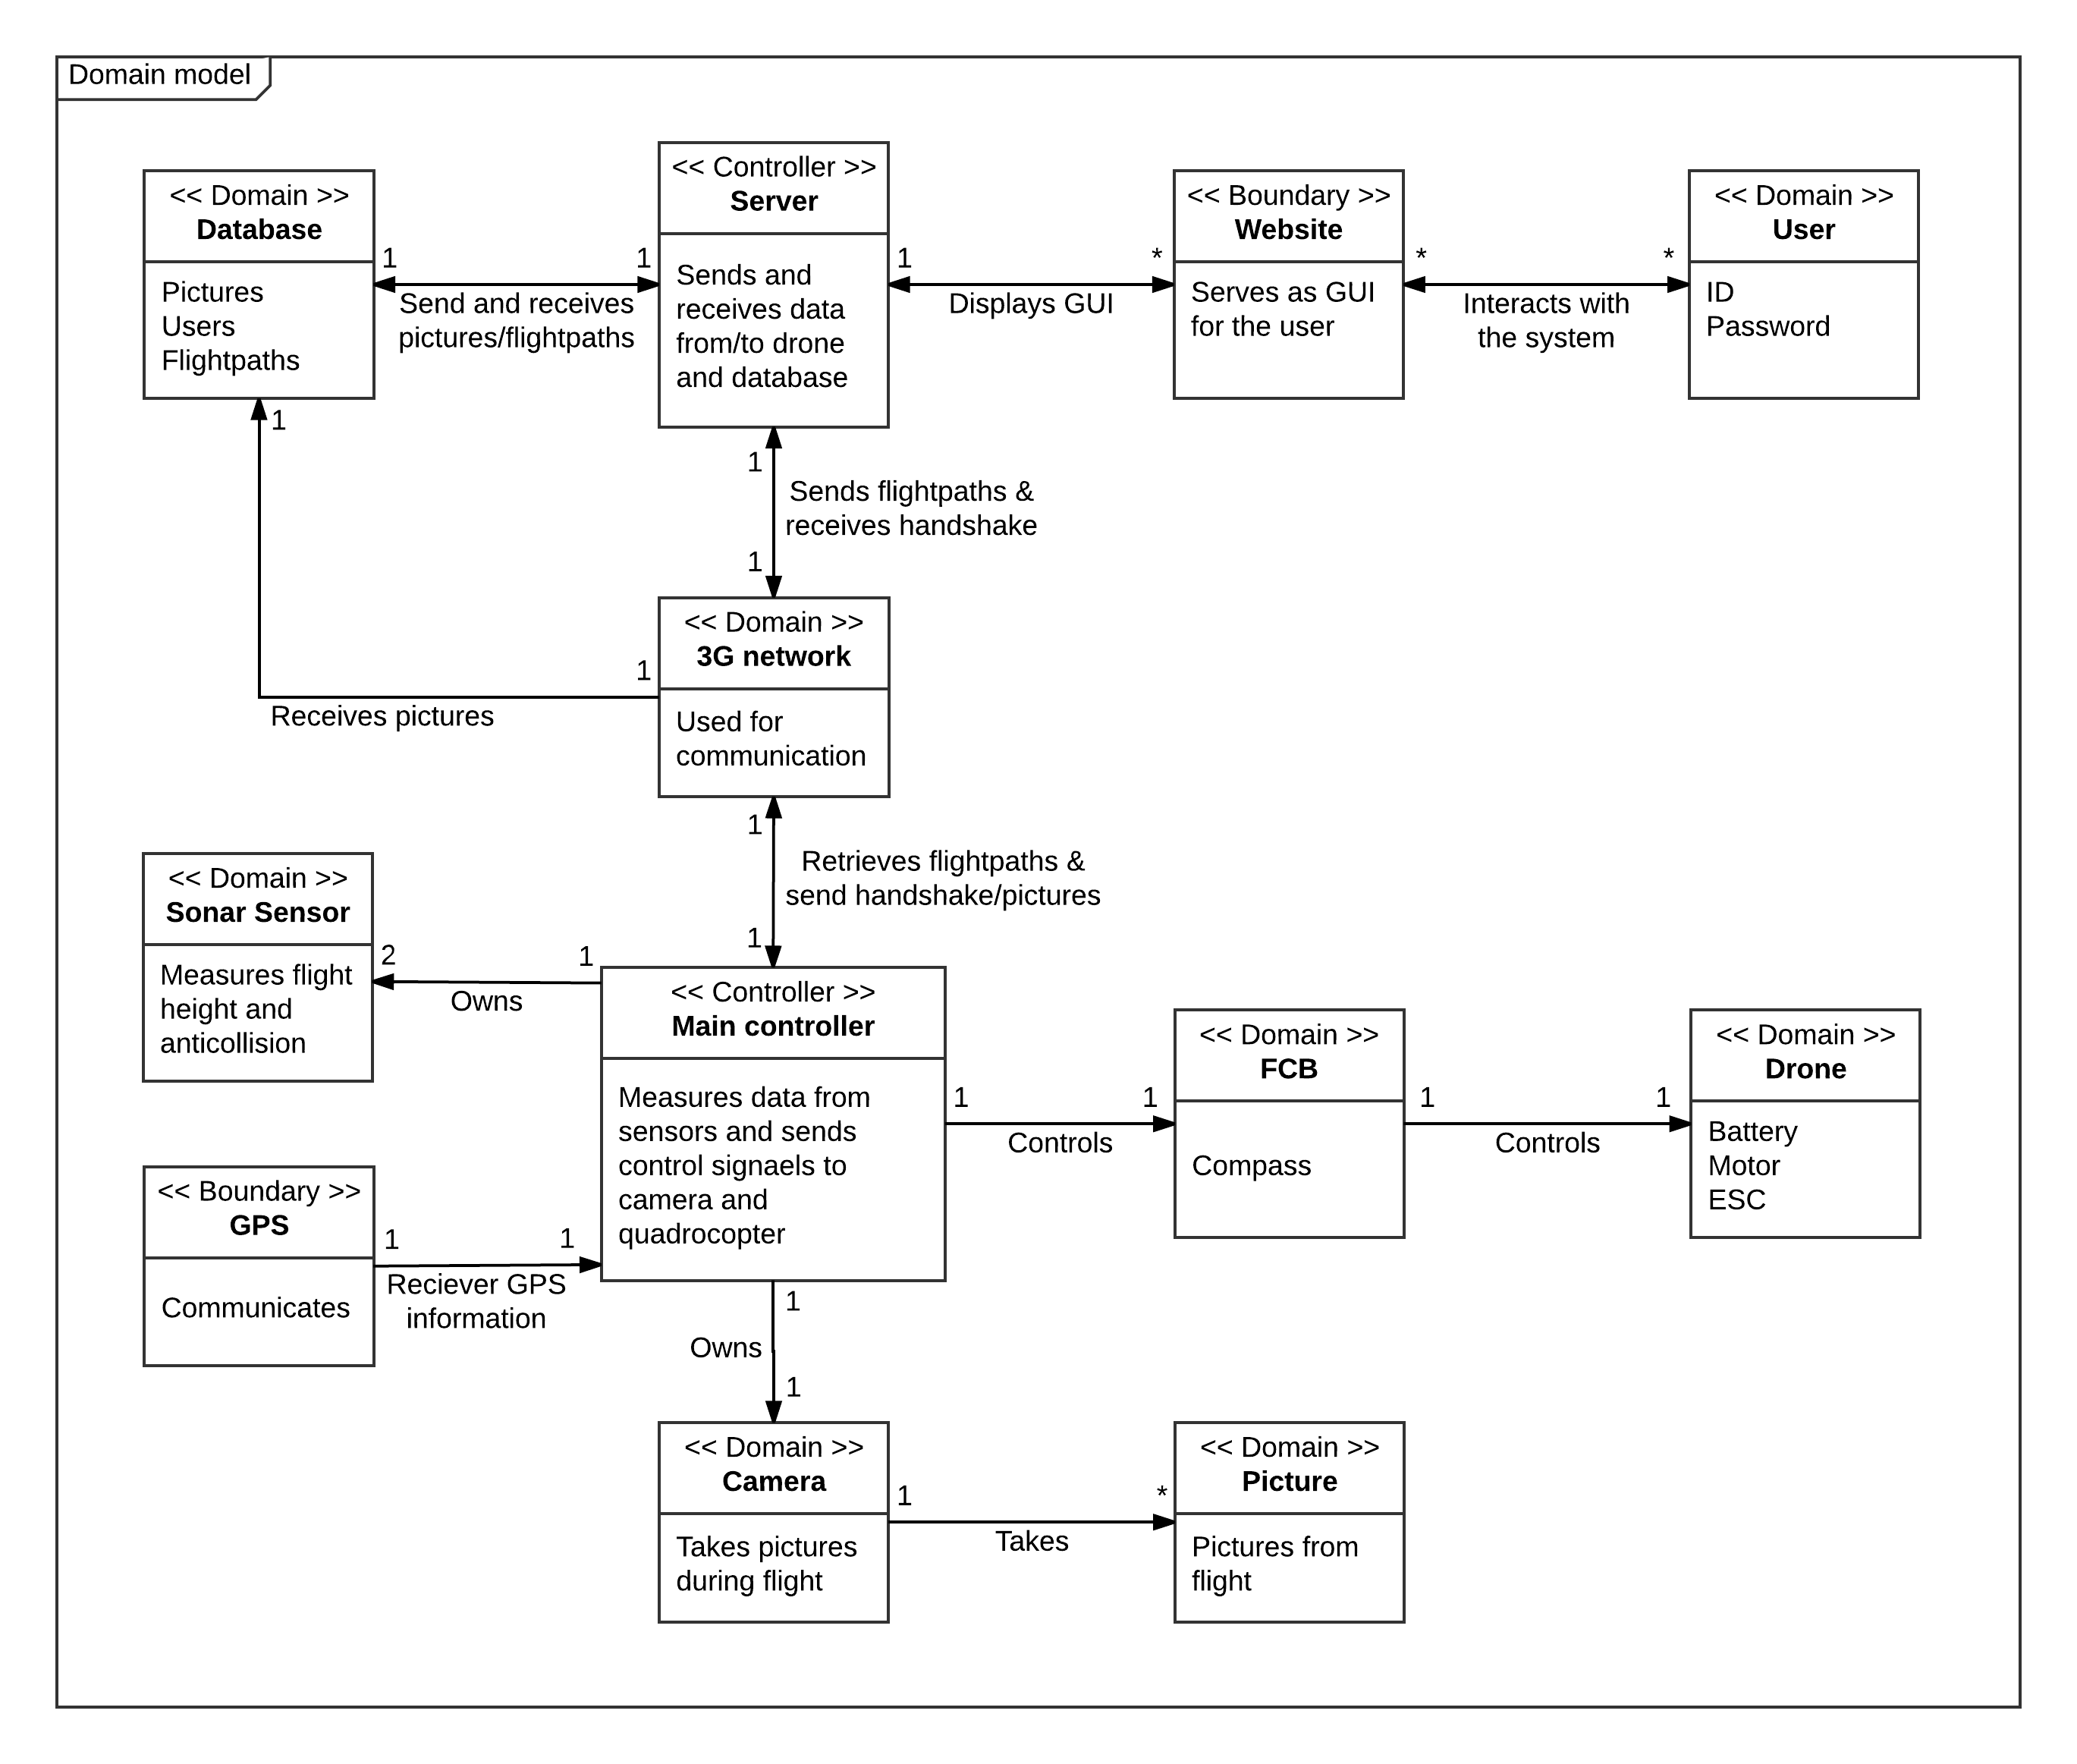
\includegraphics[width=1.\textwidth]{Billeder/domain_model.png}
	\caption{Domain model}
	\label{fig:domain_model}
\end{figure}

\newpage

Af figur \ref{fig:domain_model} ses det at domain modellen er opbygget af tre forskellige typer klasser. Nedenfor beskrives de tre forskellige klasser:

\textbf{Domain klasser}\newline
Domain klasser repræsenterer systemets domæne. Domain klasser er passive elementer, der er ansvarlige for væsentlige delparter af systemets funktionalitet.  

\textbf{Boundary klasser}\newline
Boundary klasser repræsenterer use case-aktører og aktørernes grænseflader til systemet. Boundary klasser er elementer der ligger i den yderste periferi af systemet. I nogle tilfælde er boundary klasser "front-end" elementer, der er designet til at udsende output samt at tage imod input fra systemets bruger. I andre tilfælde er boundary klasser "back-end" elementer der bruges til at hjælpe/understøtte controller klasser.

\textbf{Controller klasser} \newline
Controller klasser indeholder systemets domænelogik og står for at kontrollere systemets boundary og domain klasser. Desuden er controller klasserne ansvarlige for at håndtere input og output fra systemets boundary klasser.

\vspace{1cm}

Domain modellen bruges både til beskrivelsen af systemets hardware og software arkitektur. Men der gøres primært brug domain modellen i software arkitektur afsnittet. I software arkitekturen bruges domain modellen bla. til at danne grundlag for softwareklasser, klassenavne og klassernes indbyrdes forhold.







\section{BDD}

BDD\textunderscore generel er en beskrivelse af hele systemet, delt op i blokke.


\begin{figure}[H]
\centering
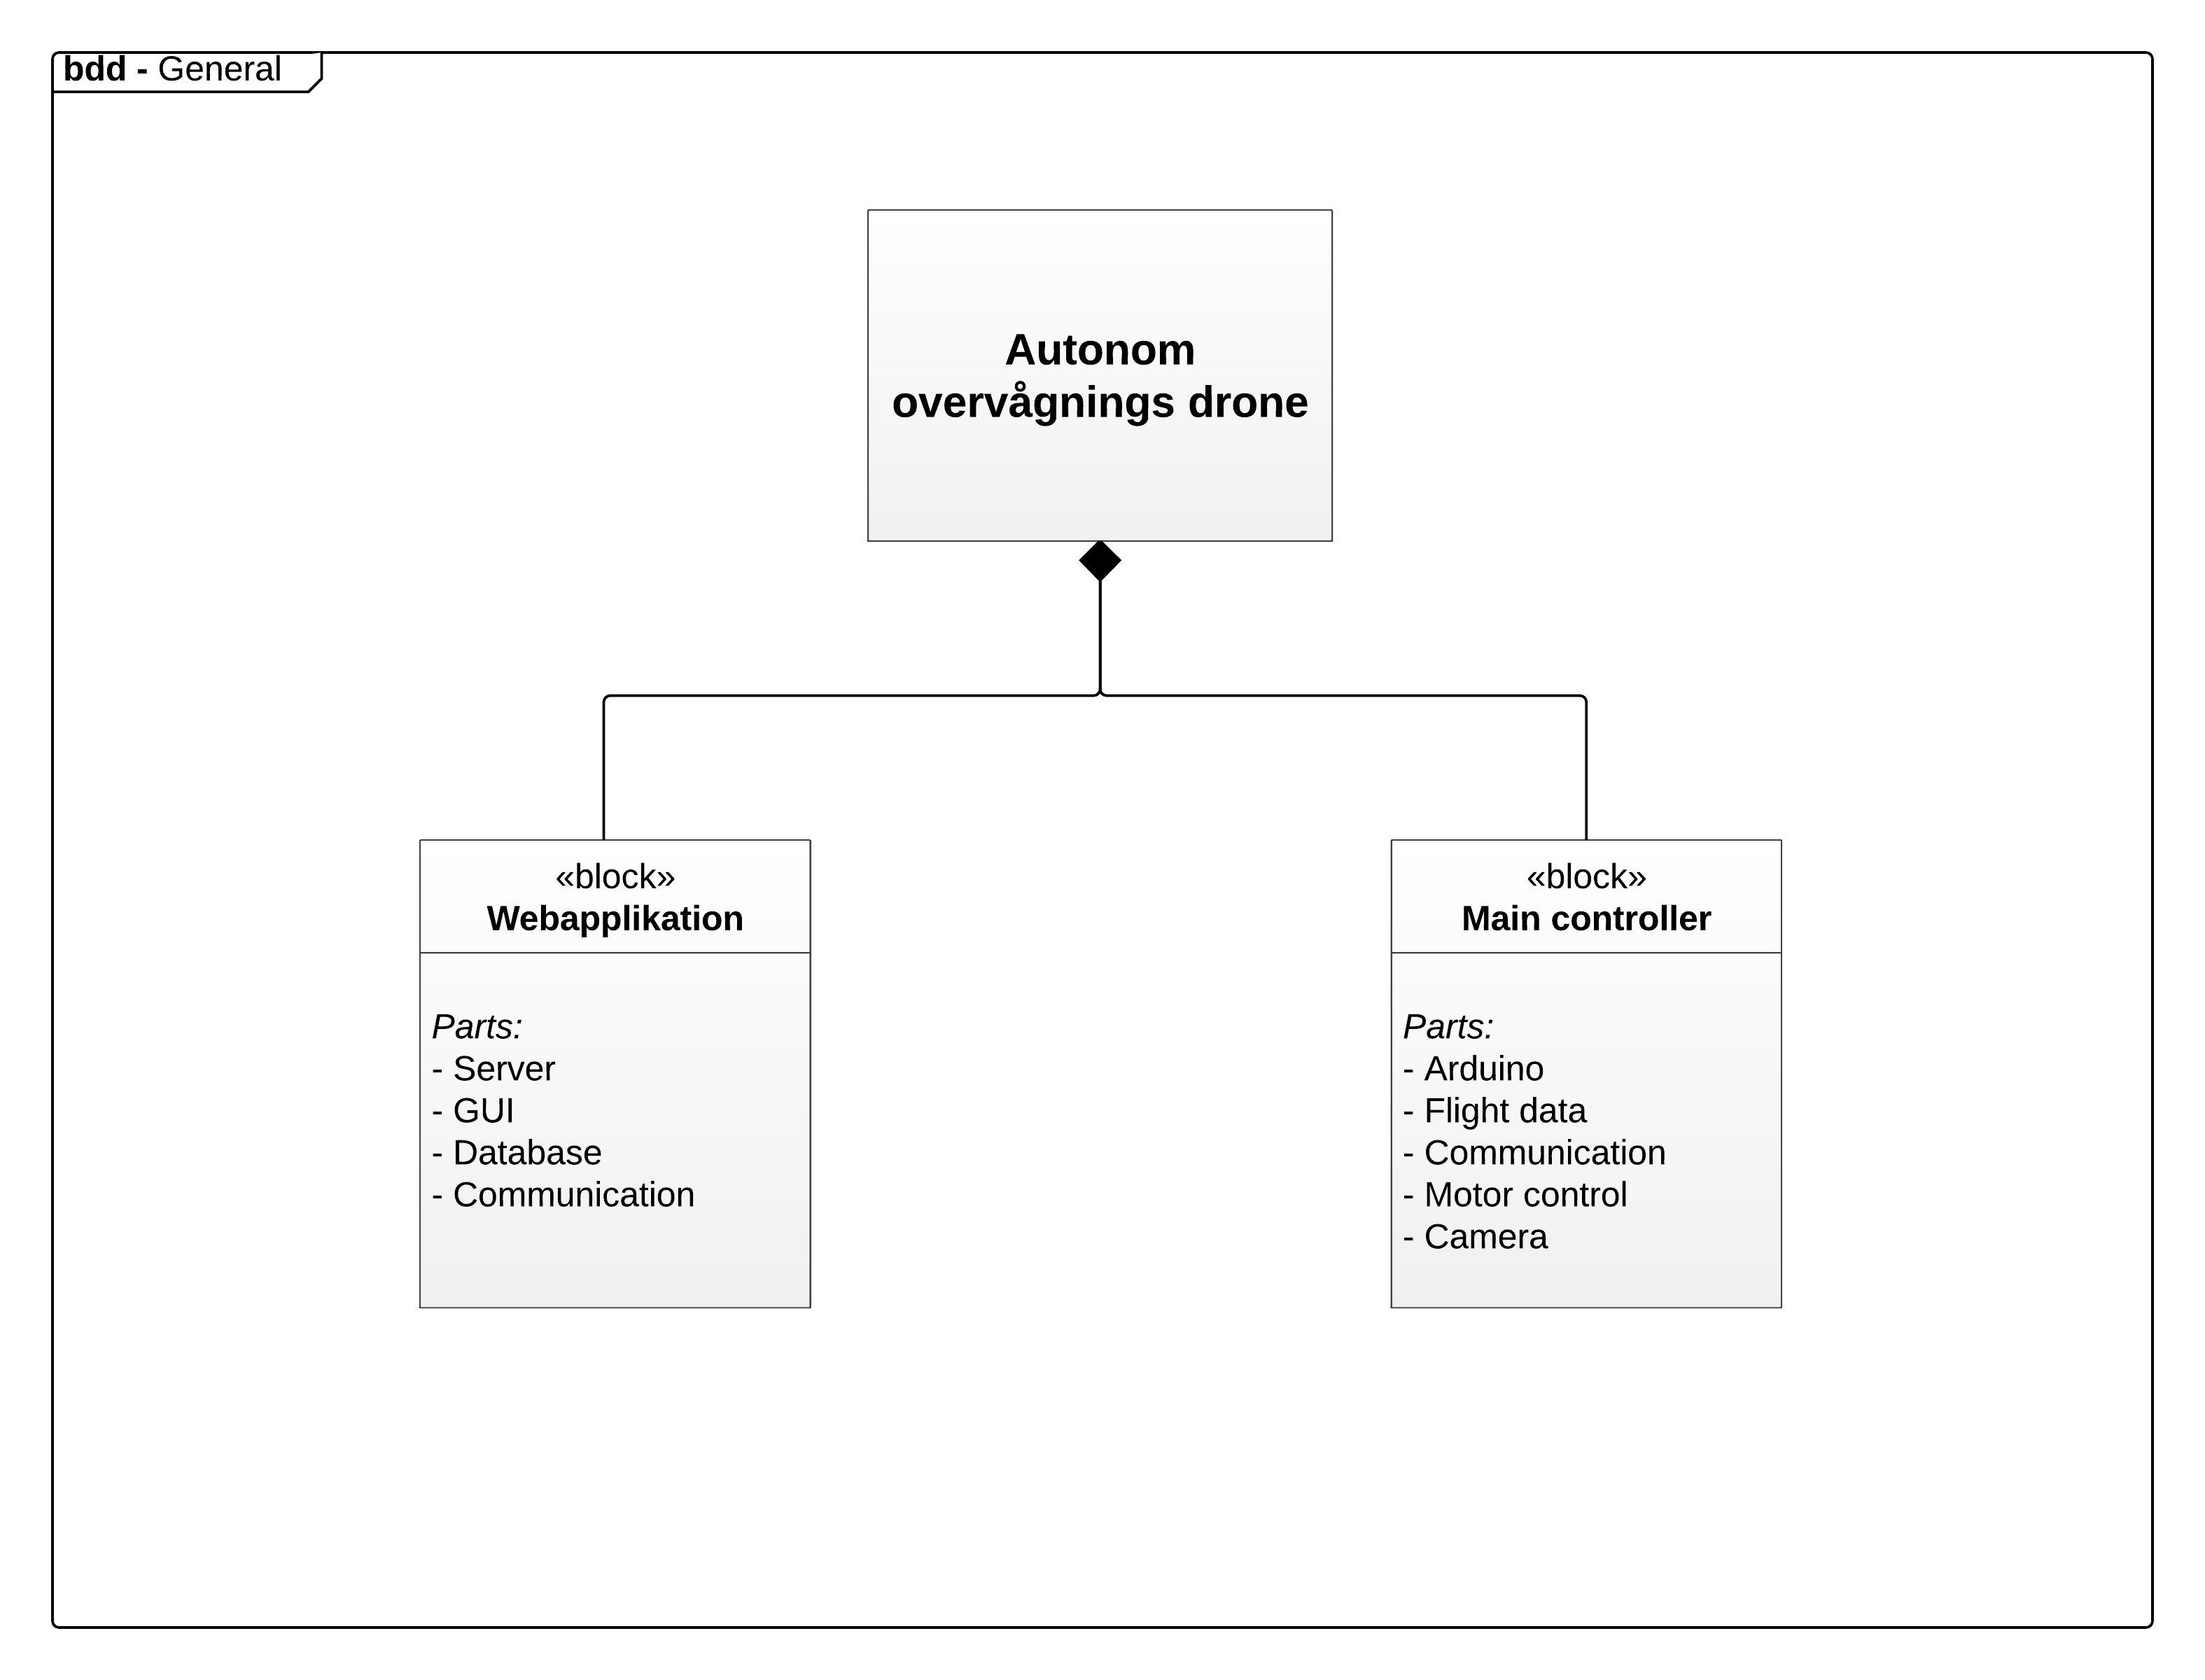
\includegraphics[width=1\textwidth]{Billeder/BDD_overordnet}
\caption{BDD - Generel}
\label{fig:bdd_generel}
\end{figure}

Dette bdd er gået mere i dybden med Main controller blokken, og viser hvilke blokke den har.

\begin{figure}[H]
\centering
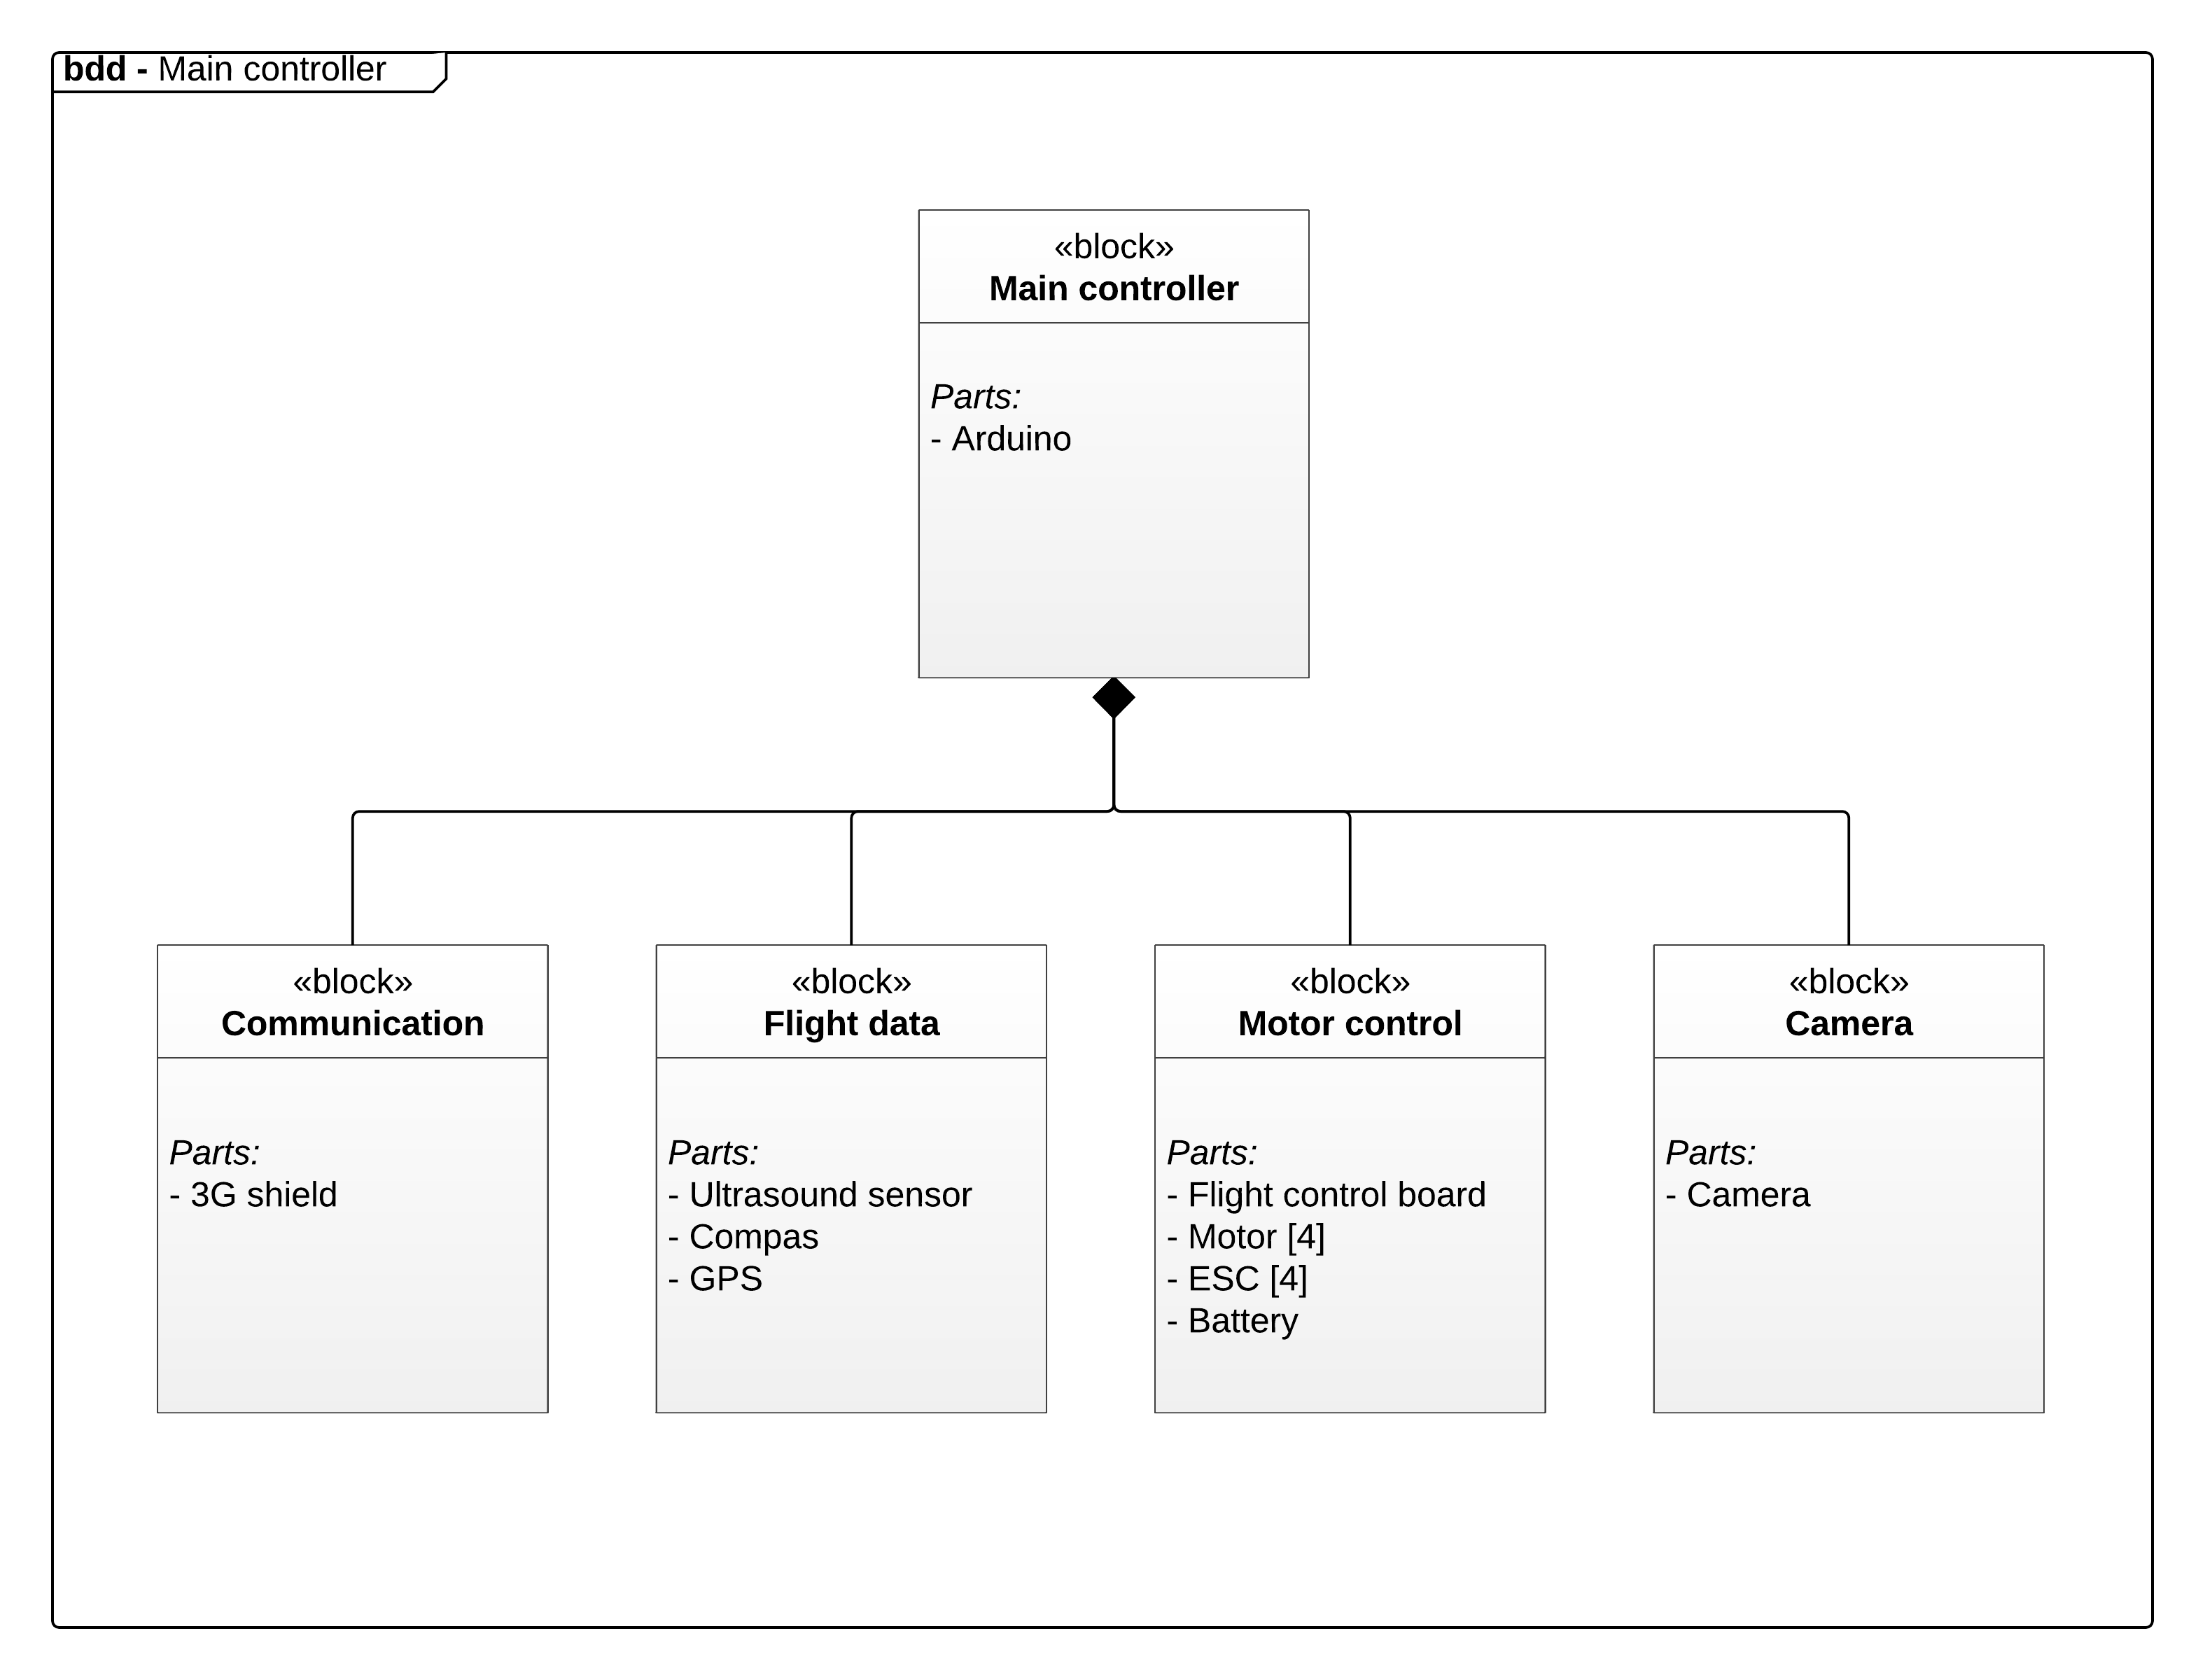
\includegraphics[width=1\textwidth]{Billeder/BDD_Maincontroller}
\caption{BDD - Main controller}
\label{fig:bdd_maincontroller}
\end{figure}

\begin{figure}[H]
\centering
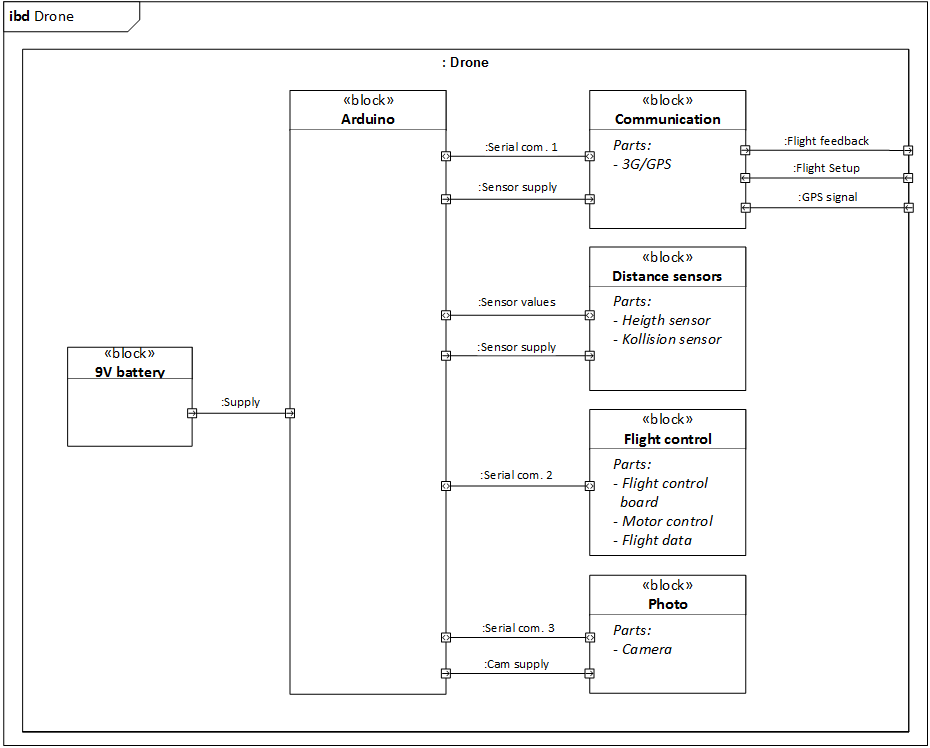
\includegraphics[width=1\textwidth]{Billeder/IBD/ibd_drone}
\caption{BDD - Main controller}
\label{fig:bdd_maincontroller}
\end{figure}


\section{Internal block diagrammer}

\subsection{Overordnet system}

På figur 2.2, på næste side, beskrives hvilke blokke der er koblet sammen samt hvilke
signaler de sender til hinanden.

\begin{figure}[H]
\centering
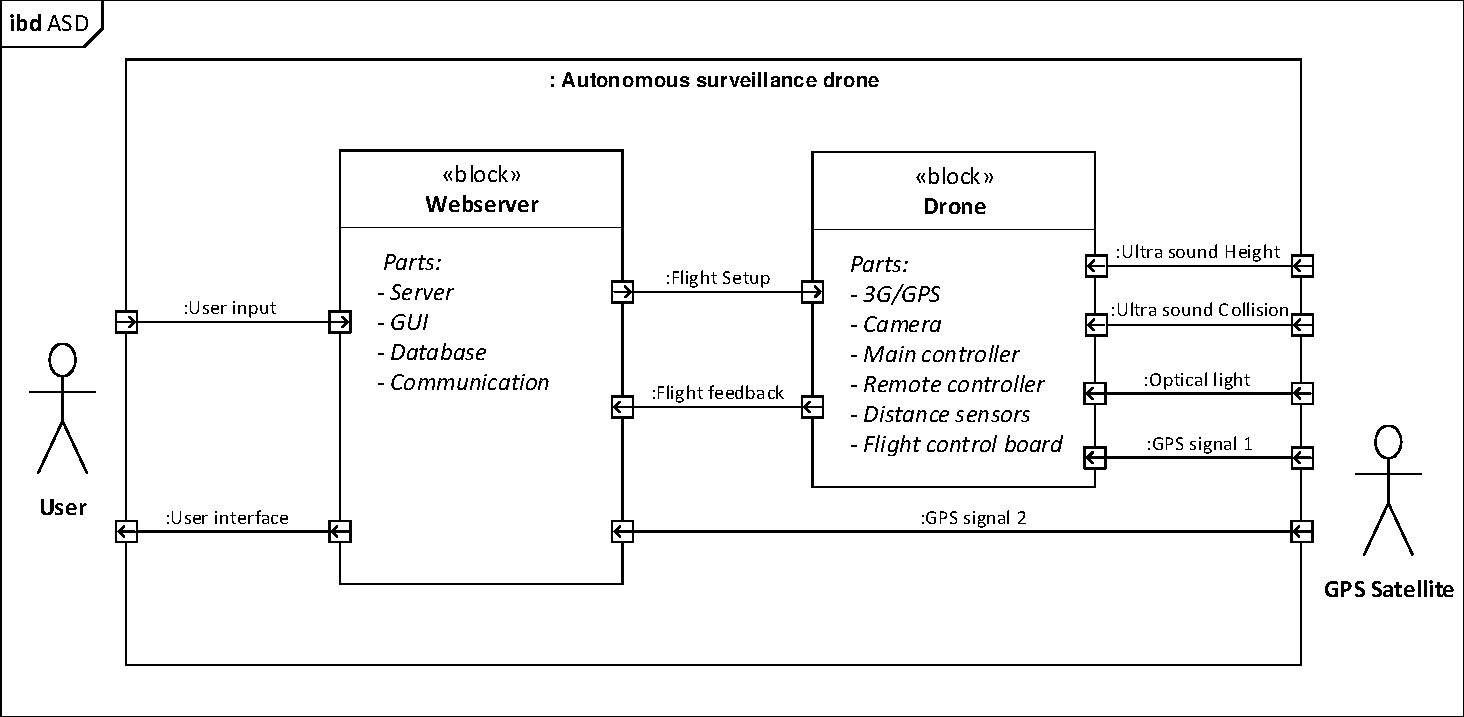
\includegraphics[width=1\textwidth]{Billeder/IBD/ibd1_overordnet.pdf}
\caption{ibd - overordnet}
\label{fig:ibd_overordnet}
\end{figure}

\begin{table}[H]
	\centering
		\begin{tabular}{|p{2.5 cm}|p{5.5 cm}|p{2.5 cm}|p{2.5 cm}|} 
		\hline
			\textbf{Signal navn} 	& \textbf{Signal beskrivelse}		& \textbf{Out} 				& \textbf{In}     \\ \hline
			User input 			& Via \textit{webapplication} opsætter bruger ny flyvning eller undersøger tidligere & Bruger 		& Webapplication.			    \\ \hline
			User interface 		& Via GUI kan bruger se hvad der sker i\textit{webapplication}.	& Webapplication.			& Bruger.				\\ \hline
			Flight setup		& Fra \textit{webapplication} sendes flyveopsætningen til dronen.	& Webapplication.	& Dronen.	\\ \hline
			Flight feedback		& Informationer fra dronen til \textit{webapplication}.	& 	Dronen.		& Webapplication.			    \\ \hline
			GPS signal 1		& GPS signal fra GPS-satellitter.	& GPS-satellit.			& Dronen.				\\ \hline
			GPS signal 2		& GPS signal fra GPS-satellitter.	& GPS-satellit.				& Webapplication.	\\ \hline  
		\end{tabular}
	\caption{Forbindelser IDB 1}
	\label{tab:IDB1}
\end{table}



\newpage
\subsection{Drone}

\begin{figure}[H]
\centering
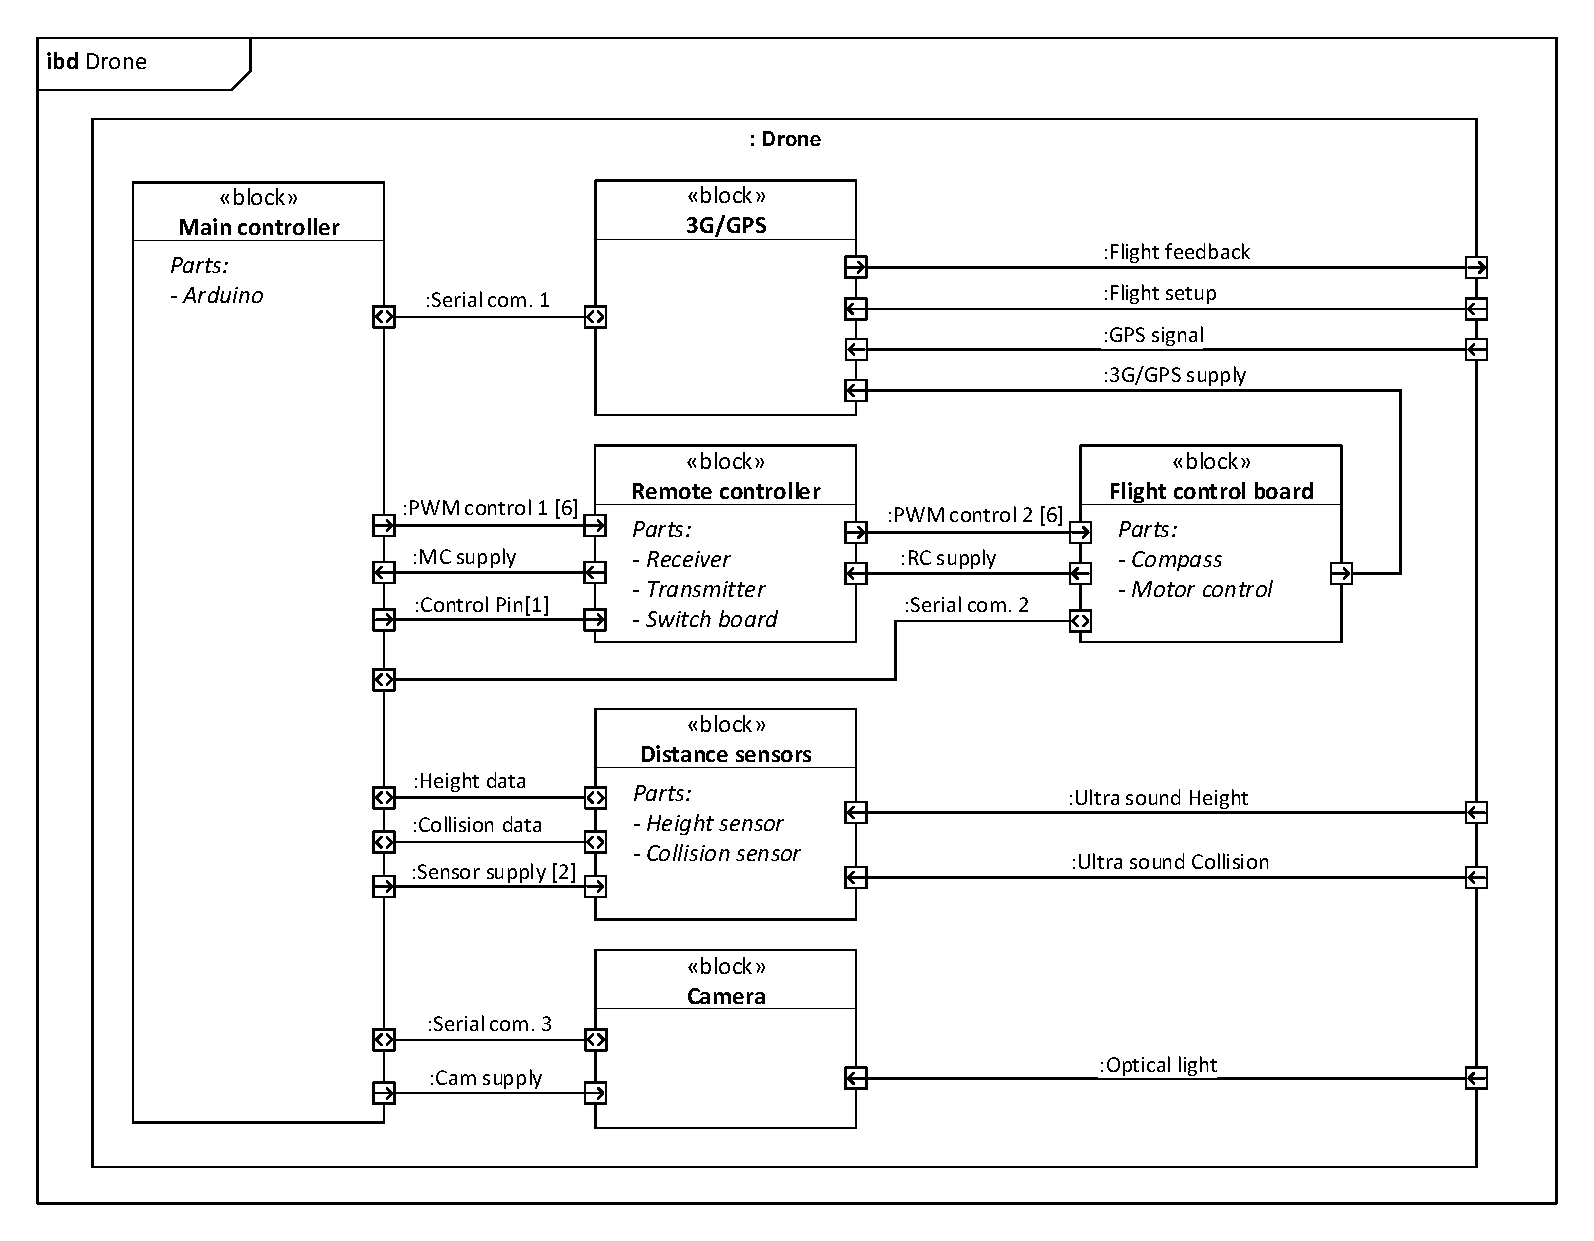
\includegraphics[width=1\textwidth]{Billeder/IBD/ibd2_drone.pdf}
\caption{ibd - drone}
\label{fig:ibd_drone}
\end{figure}

\begin{table}[H]
	\centering
		\begin{tabular}{|p{2.5 cm}|p{5.5 cm}|p{2.5 cm}|p{2.5 cm}|} 
		\hline
			\textbf{Signal navn} 	& \textbf{Signal beskrivelse}		& \textbf{Out} 				& \textbf{In}     \\ \hline
			Serial com. 1		& UART forbindelse & Main controller & 3G/GPS    \\ \hline
			Serial com. 1		& UART forbindelse & Main controller & 3G/GPS    \\ \hline
			3G/GPS supply 		& 3.2 - 4.2 V DC	& Main controller				& 3G/GPS	\\ \hline
			Flight feedback	& & 3G/GPS	& Webapplication	\\ \hline
			
			3G/GPS supply 		& 	& Webapplication				& 3G/GPS	\\ \hline
			Height data.		& Trigger \& echo signal der indikerer afstanden. 	& Main controller.	& Distance sensors.	\\ \hline
			Kollision data.		& Trigger \& echo signal der indikerer afstanden. 	& Main controller.	& Distance sensors.  \\ \hline
			Sensor supply [2]	& 5V DC	& Main controller. & Distance sensors.	\\ \hline
			Serial com. 2		& 	& Main controller				& 	\\ \hline 
			PWM control [6]		& 50 Hz 6 kanals signal.	& Main controller.				& Flight control board.	\\ \hline
			Serial com. 3		& N/A	& Main controller	& Camera	\\ \hline
			Cam supply			& N/A 	& Main controller	& Camera	\\ \hline 
		\end{tabular}
	\caption{Forbindelser til: \textbf{ibd} drone}
	\label{tab:ibddrone}
\end{table}



\newpage
\subsection{Flight control board}

På figur \ref{fig:ibd_flightcontrolboard} vises ibd til Flight control. Flight control består af Flight control board og motor control. Flight control boardet kommunikerer med main controlleren via seriel kommunikation og 6 PWM signaler. Kompas information sendes via seriel kommunikation, og PWM signalerne bestemmer hvordan motorerne skal rotere. 

\begin{figure}[H]
\centering
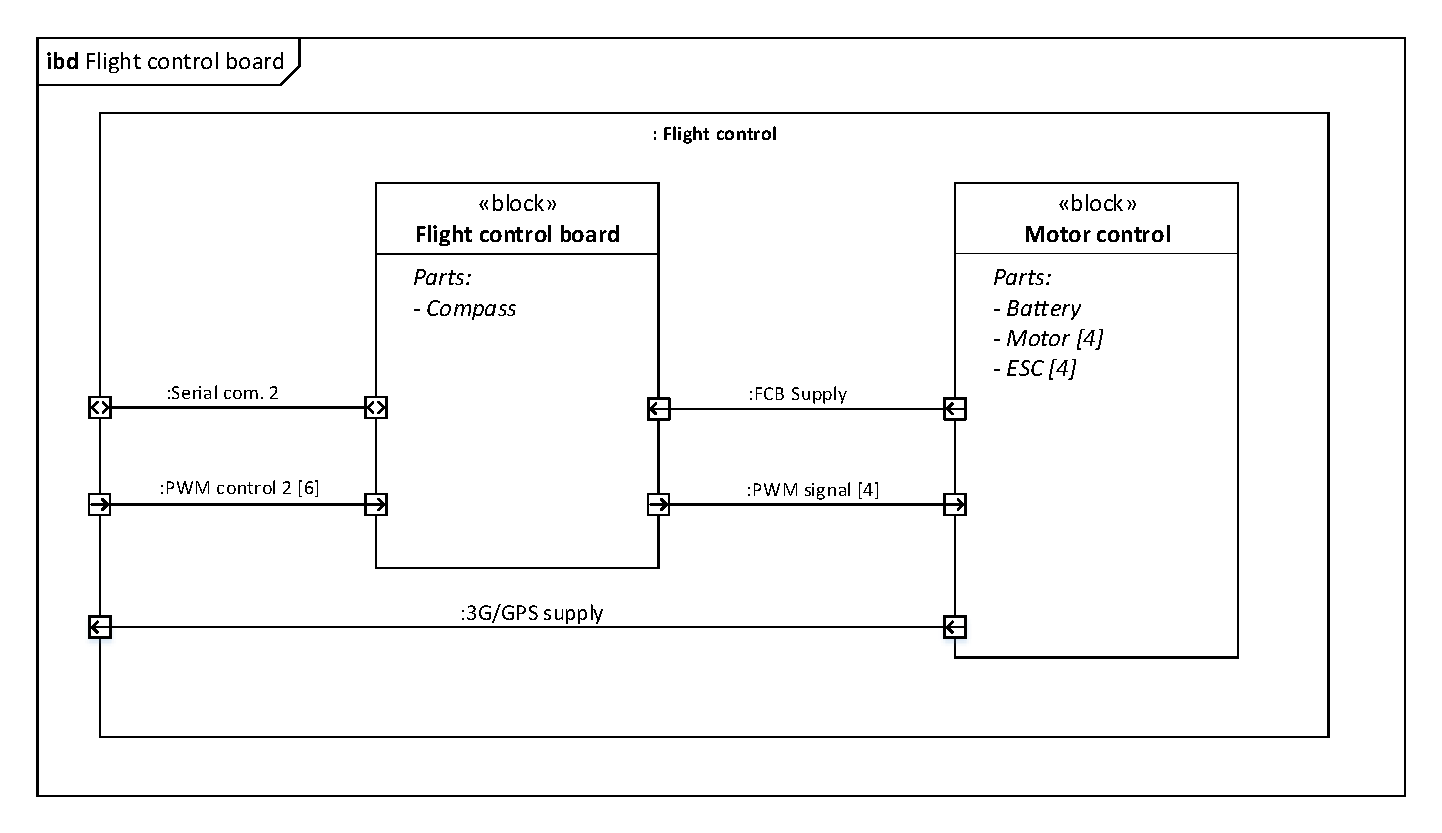
\includegraphics[width=1\textwidth]{Billeder/IBD/ibd5_flightcontrolboard.pdf}
\vspace{-0.5cm}
\caption{\textbf{ibd} - flight control board}
\label{fig:ibd_flightcontrolboard}
\end{figure}

\vspace{0.5cm}

\begin{table}[H]
	\centering
		\begin{tabular}{|p{3.2 cm}|p{5.2 cm}|p{2.4 cm}|p{2.4 cm}|} 
		\hline
			\textbf{Signal navn} 	& \textbf{Signal beskrivelse}		& \textbf{Out} 				& \textbf{In}     \\ \hline
			Serial com. 2 & RX / TX. signal. & Arduino. & Flight control board.			    \\ \hline
			PWM control 2 [6] & 6 PWM signaler. \newline Enten 244 Hz eller 50 Hz & Arduino. & Flight control board.				\\ \hline
			FCB supply &  Forsyning til flight contorl \newline boardet. 5V DC & Motor control. & Flight control board.	\\ \hline
			PWM signal [4] & 400 Hz 4 kanals signal. \newline Duty cycle mellem 40-80 $\%$. & Fligt control board. & Motor control.   \\ \hline 
			RC supply & 5V forsyning. & Flight control board. & Remote \newline controller.  \\ \hline 
		\end{tabular}
	\caption{Forbindelser til: \textbf{Ibd} - flight control board. }
	\label{tab:ibd_Flight_control_board}
\end{table}





\newpage
\subsection{Remote controller}

På figur \ref{fig:ibd_remotecontroller} vises ibd til Remote controller, der består af receiver, transmitter og switch board. Blokken gør det muligt at switche mellem autonom og manuel styring. Afhængig af det signal receiver blokken modtager fra transmitter benyttes henholdsvis manuel eller autonom flyvning. Når der flyves autonom, benyttes PWM signaler fra main controller til styring, og under manuel flyvning benyttes signaler fra receiver.

\begin{figure}[H]
\centering
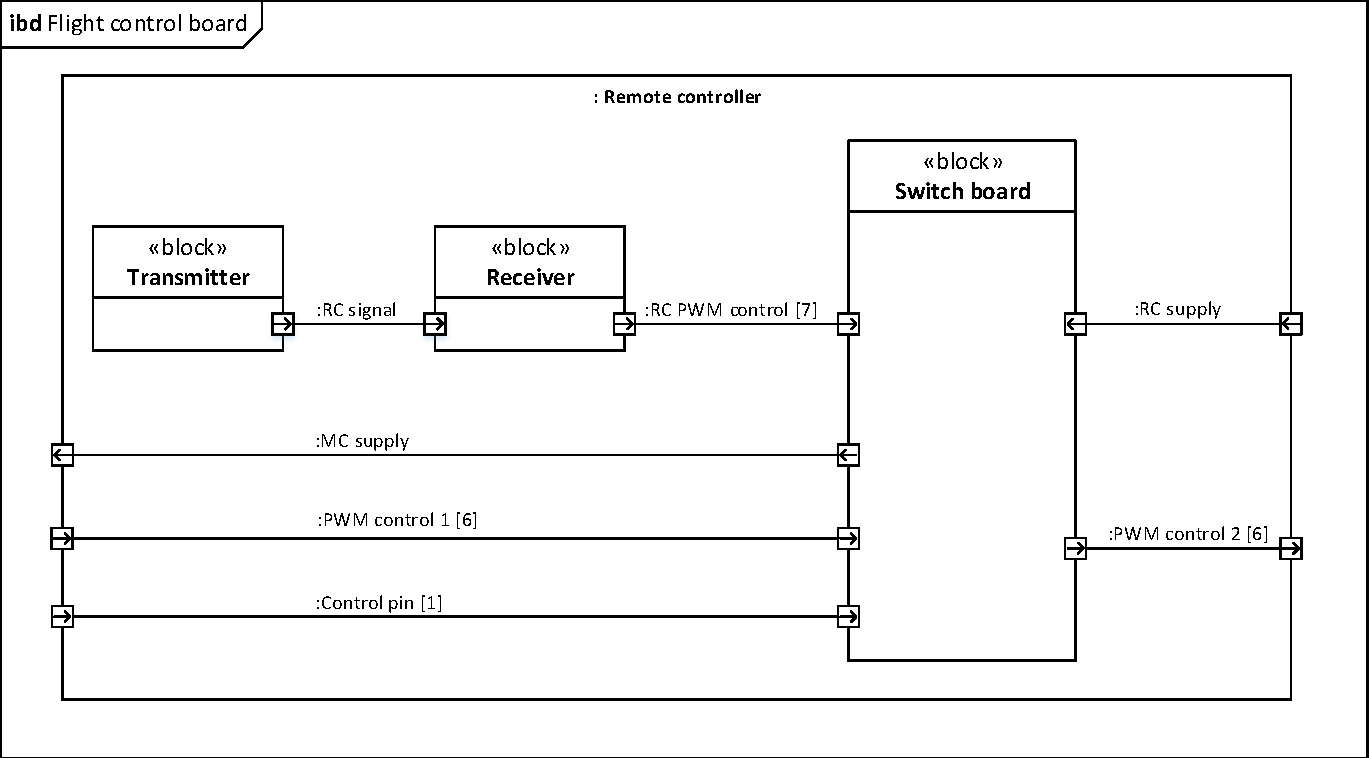
\includegraphics[width=1\textwidth]{Billeder/IBD/ibd7_remotecontroller.pdf}
\vspace{-1cm}
\caption{Ibd - Remote controller}
\label{fig:ibd_remotecontroller}
\end{figure}

\begin{table}[H]
	\centering
		\begin{tabular}{|p{3.5 cm}|p{4.5 cm}|p{2.6 cm}|p{2.6 cm}|} 
		\hline
			\textbf{Signal navn} 	& \textbf{Signal beskrivelse}		& \textbf{Out} 				& \textbf{In}     \\ \hline
			RC supply & 5V DC til switch board. & Flight control board. & Switch board.	\\ \hline	
			PWM control 2 [6] & 6 PWM signaler. \newline Enten 244 Hz eller 50 Hz & Switch board. & Flight control board.				\\ \hline
					
			RC PWM control [7] & 6 PWM signaler på 50 Hz \newline + GND & Reciever. & Switch board.				\\ \hline
			RC signal & 2,4 GHz trådløs \newline kommunikation & Reciever. & Switch board.				\\ \hline
			
			MC supply 			& 5V DC. 						& Switch board.  & Main \newline controller.	\\ \hline
			PWM control 1 [6] 	& 6 PWM signaler på 244 Hz. 	& Main controller. & Switch board. \\ \hline
			Control pin [1]		& Skifter mellem 5V og 0V		& Main controller	& Remoto \newline  controller.    \\ \hline
		\end{tabular}
	\caption{Forbindelser til: Ibd - remote controller. }
	\label{tab:ibd_remote_controller}
\end{table}





\newpage
\subsection{Afstandssensorer}

På figur \ref{fig:ibd_distancesensor} vises et ibd over afstandssensor blokken. 
Blokken består af to forskellige sensorer, en sensor til højde måling og en til antikollision. Begge sensorer fungerer uafhængig af hinanden, de aktiveres enkeltvis når main controller sender trigger signal til dem.   

\begin{figure}[H]
\centering
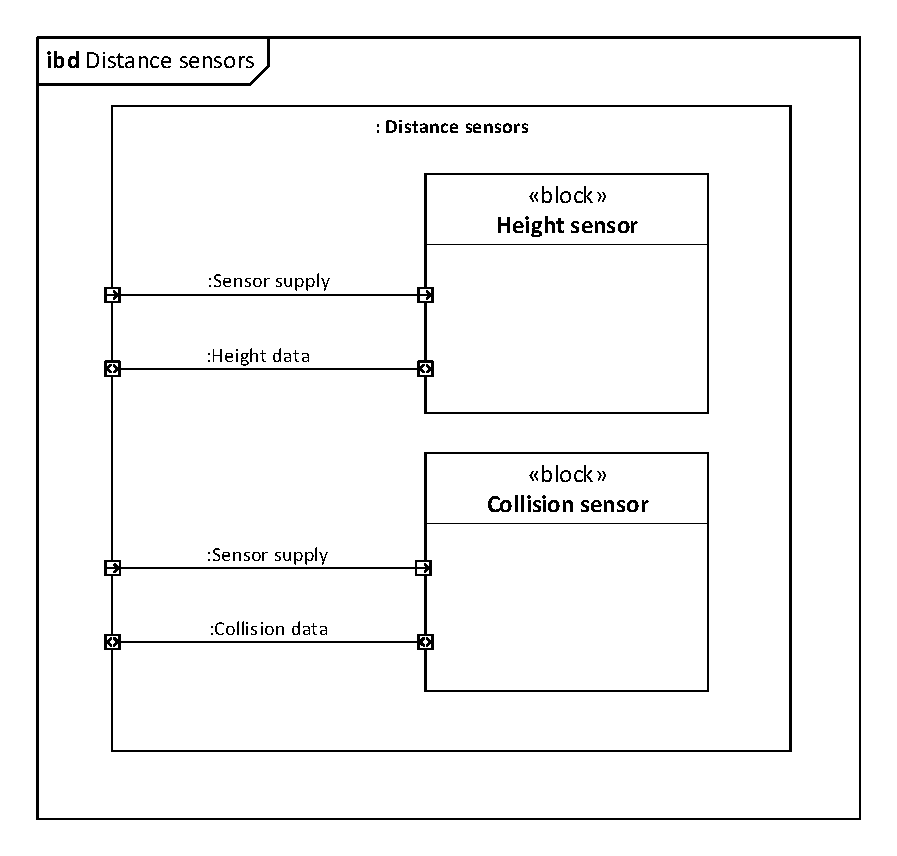
\includegraphics[width=1\textwidth]{Billeder/IBD/ibd4_distancesensor.pdf}
\vspace{-1cm}
\caption{ibd - distance sensor}
\label{fig:ibd_distancesensor}
\end{figure}

\begin{table}[H]
	\centering
		\begin{tabular}{|p{2.6 cm}|p{4.9 cm}|p{2.5 cm}|p{2.5 cm}|} 
		\hline
			\textbf{Signal navn} 	& \textbf{Signal beskrivelse}		& \textbf{Out} 				& \textbf{In}     \\ \hline
			Sensor supply & 5V DC.  & Arduino. & Height sensor.  \\ \hline
			Height data & RX / TX signal. & Arduino.	& Height sensor.	\\ \hline
			Sensor supply & 5V DC. & Arduino. & Collision sensor.	\\ \hline
			Collision data & RX /TX signal & Arduino. & Collision sensor.			    \\ \hline  
		\end{tabular}
	\caption{Forbindelser til: \textbf{ibd} Distance sensor}
	\label{tab:IBDDistancesensor}
\end{table}


\newpage
\subsection{Motor styring}

På figur \ref{fig:ibd_motorcontrol} vises det interne blok diagram for motor control blokken. Blokken består af 4 ESC'er, 4 motorer og et 12V batteri. 12V batteriet står for forsyning til hele blokkken, mens de PWM signaler der sendes ind i ESC'erne bestemmer hvor meget forsyning motorerne tildeles. Den PWM der sendes til ESC'er sendes med en duty cycle mellem 40-80\%. Ved ændring af duty cyclen, ændres forsyningen til dronens motorer. Ved en ændring af forsyning ændres hastigheden hvorved motorerne roterer.

\begin{figure}[H]
\centering
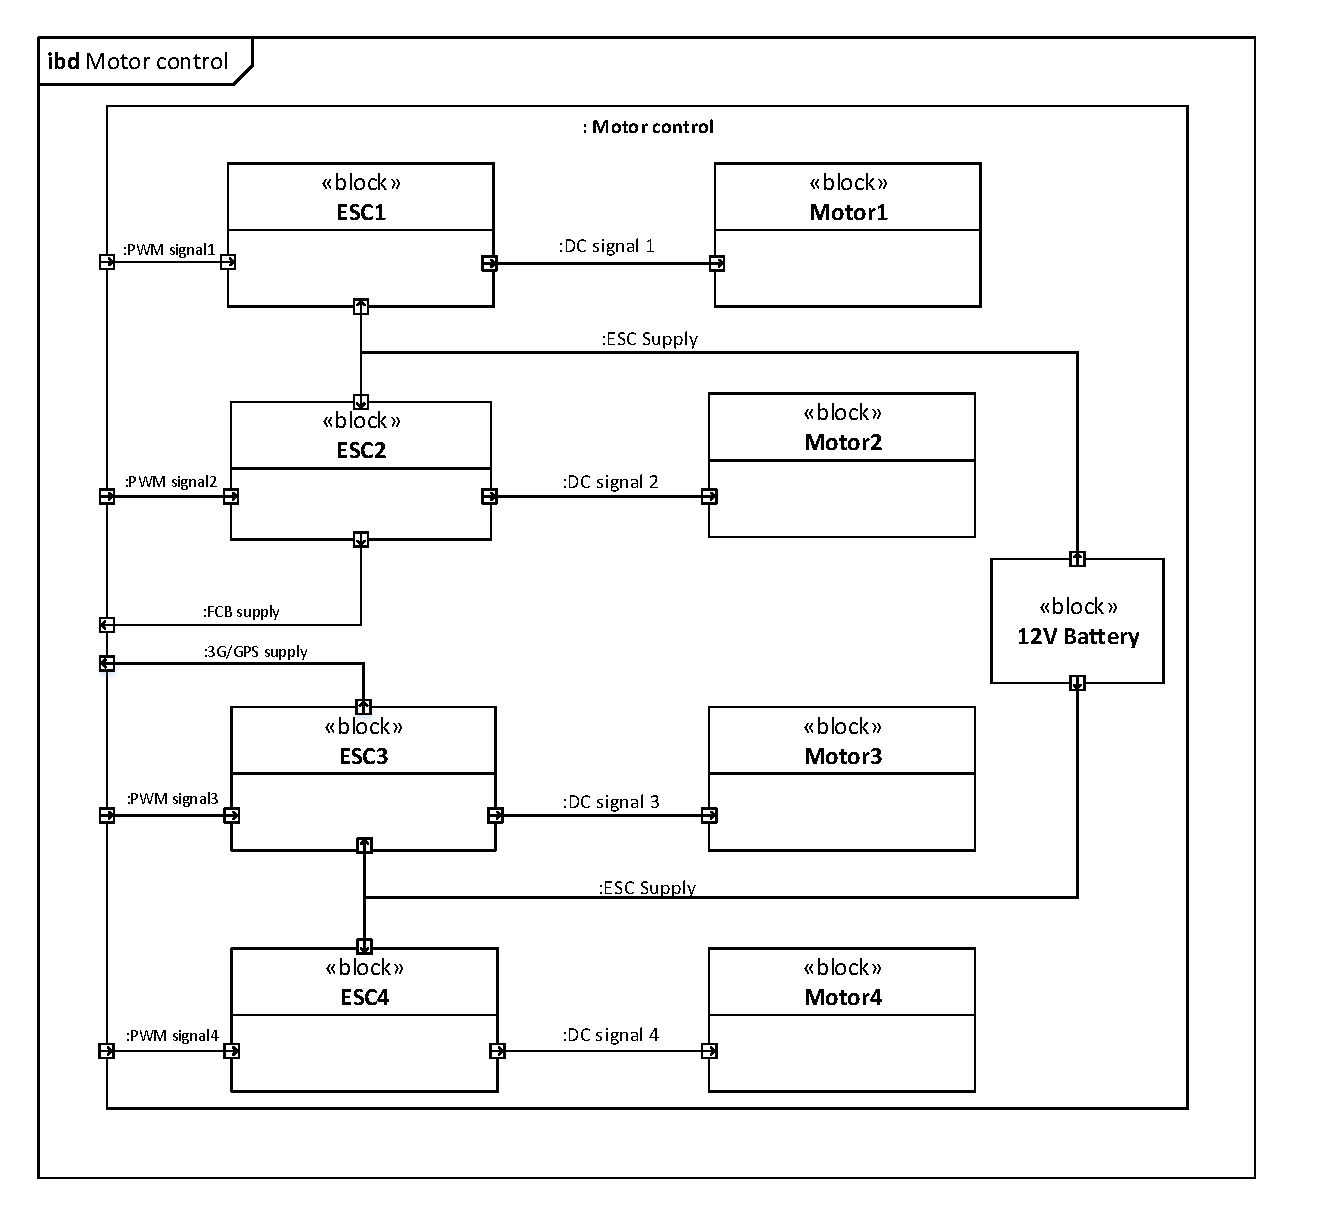
\includegraphics[width=1\textwidth]{Billeder/IBD/ibd6_motorcontrol.pdf}
\vspace{-0.5cm}
\caption{\textbf{Ibd} - Motor control}
\label{fig:ibd_motorcontrol}
\end{figure}

\begin{table}[H]
	\centering
		\begin{tabular}{|p{2.7 cm}|p{5.5 cm}|p{2.5 cm}|p{2.5 cm}|} 
		\hline
			\textbf{Signal navn} 	& \textbf{Signal beskrivelse}		& \textbf{Out} 				& \textbf{In}     \\ \hline
			PWM signal1 & 400 Hz signal med en duty cycle på 40-80 $\%$ & Flight control. & ESC1.	\\ \hline
			PWM signal2 & 400 Hz signal med en duty cycle på 40-80 $\%$ & Flight control. & ESC2.	\\ \hline
			PWM signal3 & 400 Hz signal med en duty cycle på 40-80 $\%$ & Flight control. &	ESC3. \\ \hline
			PWM signal4 & 400 Hz signal med en duty cycle på 40-80 $\%$ & Flight control. & ESC4. \\ \hline
			DC signal 1 & Et varierende DC. & ESC1. & Motor1.	\\ \hline
			DC signal 2 & Et varierende DC. & ESC2. & Motor2.	\\ \hline
			DC signal 3 & Et varierende DC. & ESC3. & Motor3.	\\ \hline
			DC signal 4 & Et varierende DC. & ESC4. & Motor4.	\\ \hline
			FCB supply & 5V DC. & ESC2 & Flight control.	\\ \hline
			3G/GPS supply & 5V DC. & ESC3. & 3G/GPS module.	\\ \hline
			ESC supply & 12V DC. & Battery. & ESC1/ESC2.	\\ \hline
			ESC supply & 12V DC. & Battery. & ESC3/ESC4.	\\ \hline
			
		\end{tabular}
	\caption{Forbindelser til: \textbf{Ibd} - Motor control}
	\label{tab:IBD_Motor_control}
\end{table}




\subsection{Hardware design Switch board}
I det følgende afsnit beskrives designet af hardwaren til switch boardet. Switch boardet er udviklet således at fjernbetjeningen kan overtage styringen fra main controlleren.

På figur \ref{fig:switchboard_design} ses det overordnede design til switch boardet. 
De respektive PWM signaler skal ind i en 2-input AND gate hvor hver PWM signal har en AND gate. Den anden indgang bruges af et kontrol pin som styres af main controlleren. Denne pin sættes enten høj eller lav, afhængigt af hvilken enhed der skal styre dronen. 
De AND gates der har med samme PWM styring at gøre (fx. Throttle) sendes til en OR gate som sender PWM signalet videre til flight control boardet. 

\begin{figure}[H]
	\centering
	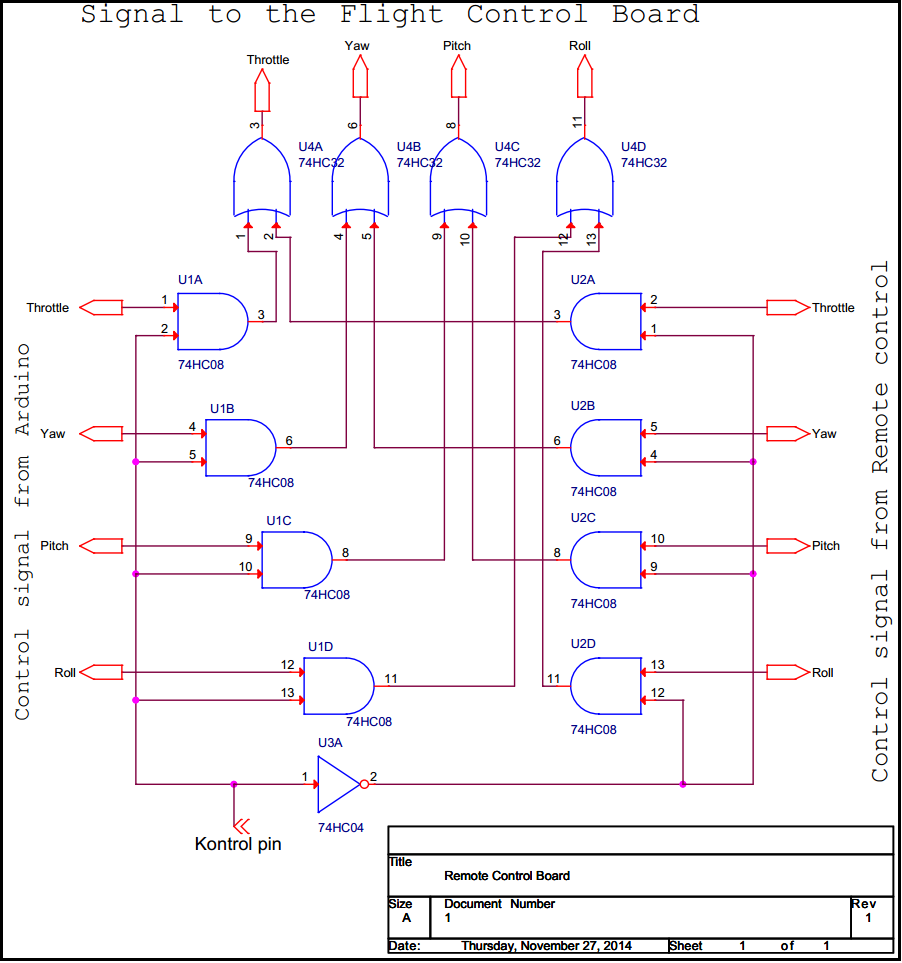
\includegraphics[width=1\textwidth]{Billeder/hardware/switch_board_diagram.png}
	\caption{Switch board design}
	\label{fig:switchboard_design}
\end{figure}


\chapter{Software}

I det følgende afsnit beskrives systemet software vha. UML diagrammer. Afsnittet er opdelt i to dele, en del der beskæftiger sig med software tilhørende webapplikation og en del med software til dronen. 

Indledningsvis vises design overview diagrammer, disse bruges til at danne overblink over hvordan webapplikationen skal reagere på input fra bruger. Herefter vises pakkediagrammer med tilhørende beskrivelser. De pakker der vises i pakkediagrammerne består af en eller flere klasser, der med stort samspil udfører opgaver indenfor et fælles ansvarsområde. Efter pakkediagrammerne vises en række klassediagrammer, disse bruges til at vise struktur og sammenhæng mellem pakkernes forskellige klasser, eksempelvis arv.

\newpage
\section{Design overview diagrammer}

I dette afsnit vises design overview diagrammer, som bruges til at definere hvordan systemet skal reagerer på input fra bruger.

\vspace{-5pt}
\begin{figure}[H]
	\centering
	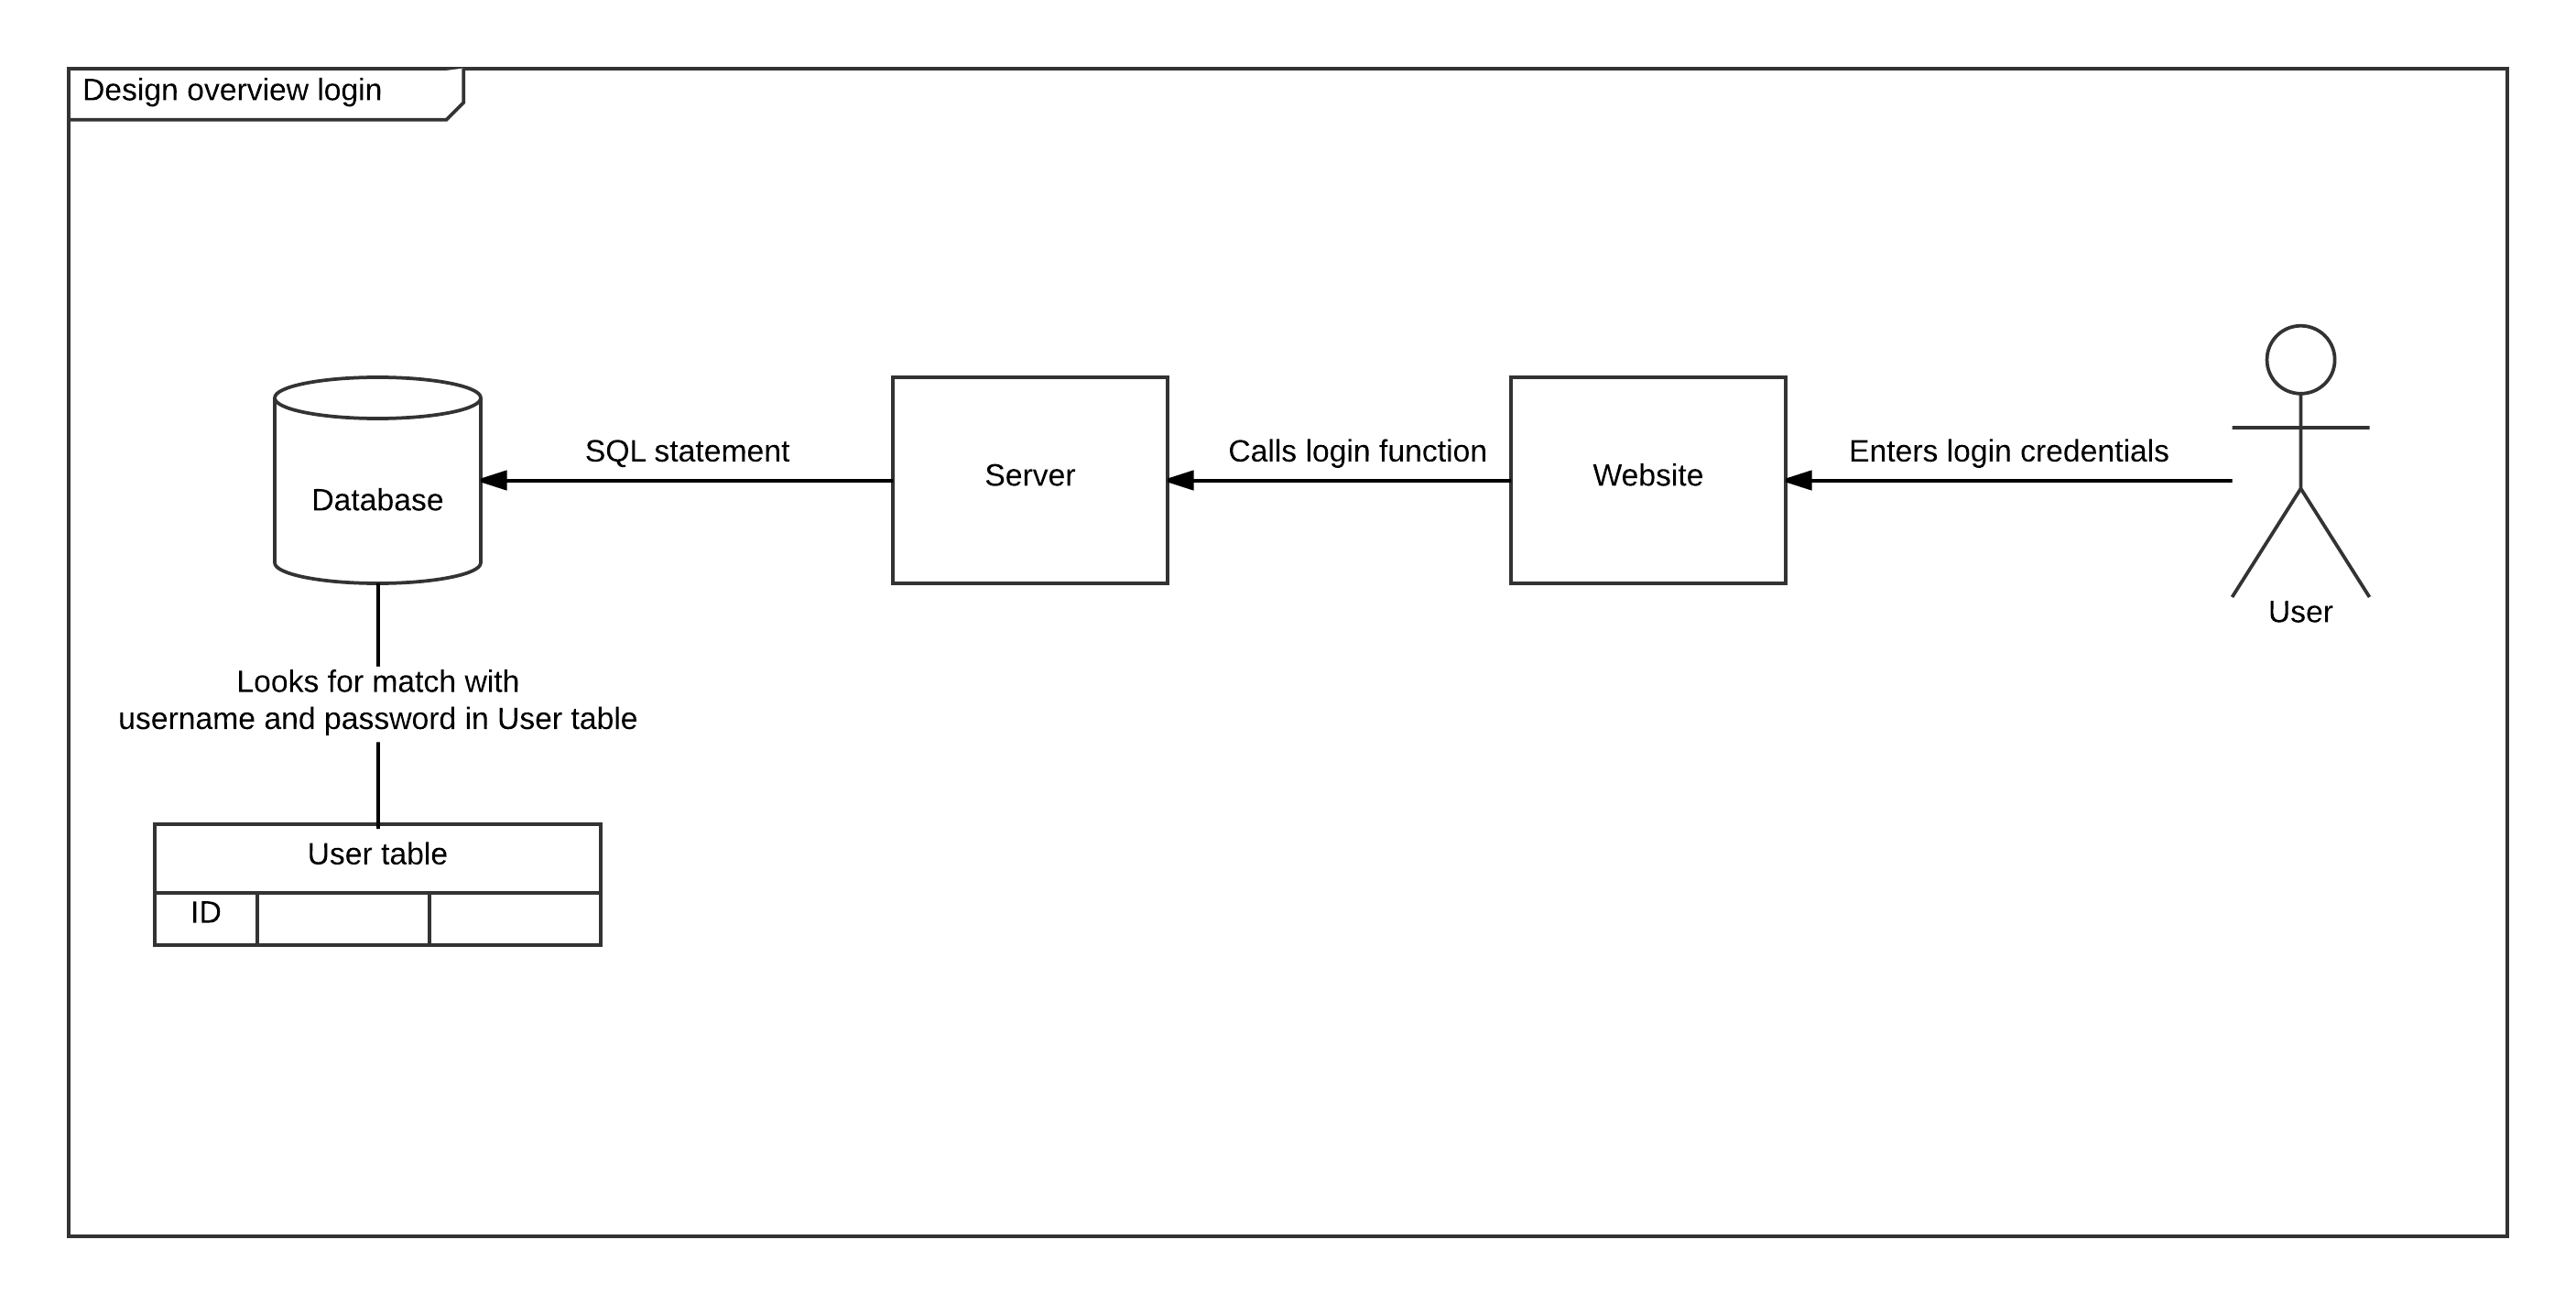
\includegraphics[width=1\textwidth]{Billeder/Design_overview/design_overview_login}
	\vspace{-1cm}
	\caption{Design overview - login}
	\label{fig:pakke_diagram}
\end{figure}

\vspace{-5pt}
\begin{figure}[H]
	\centering
	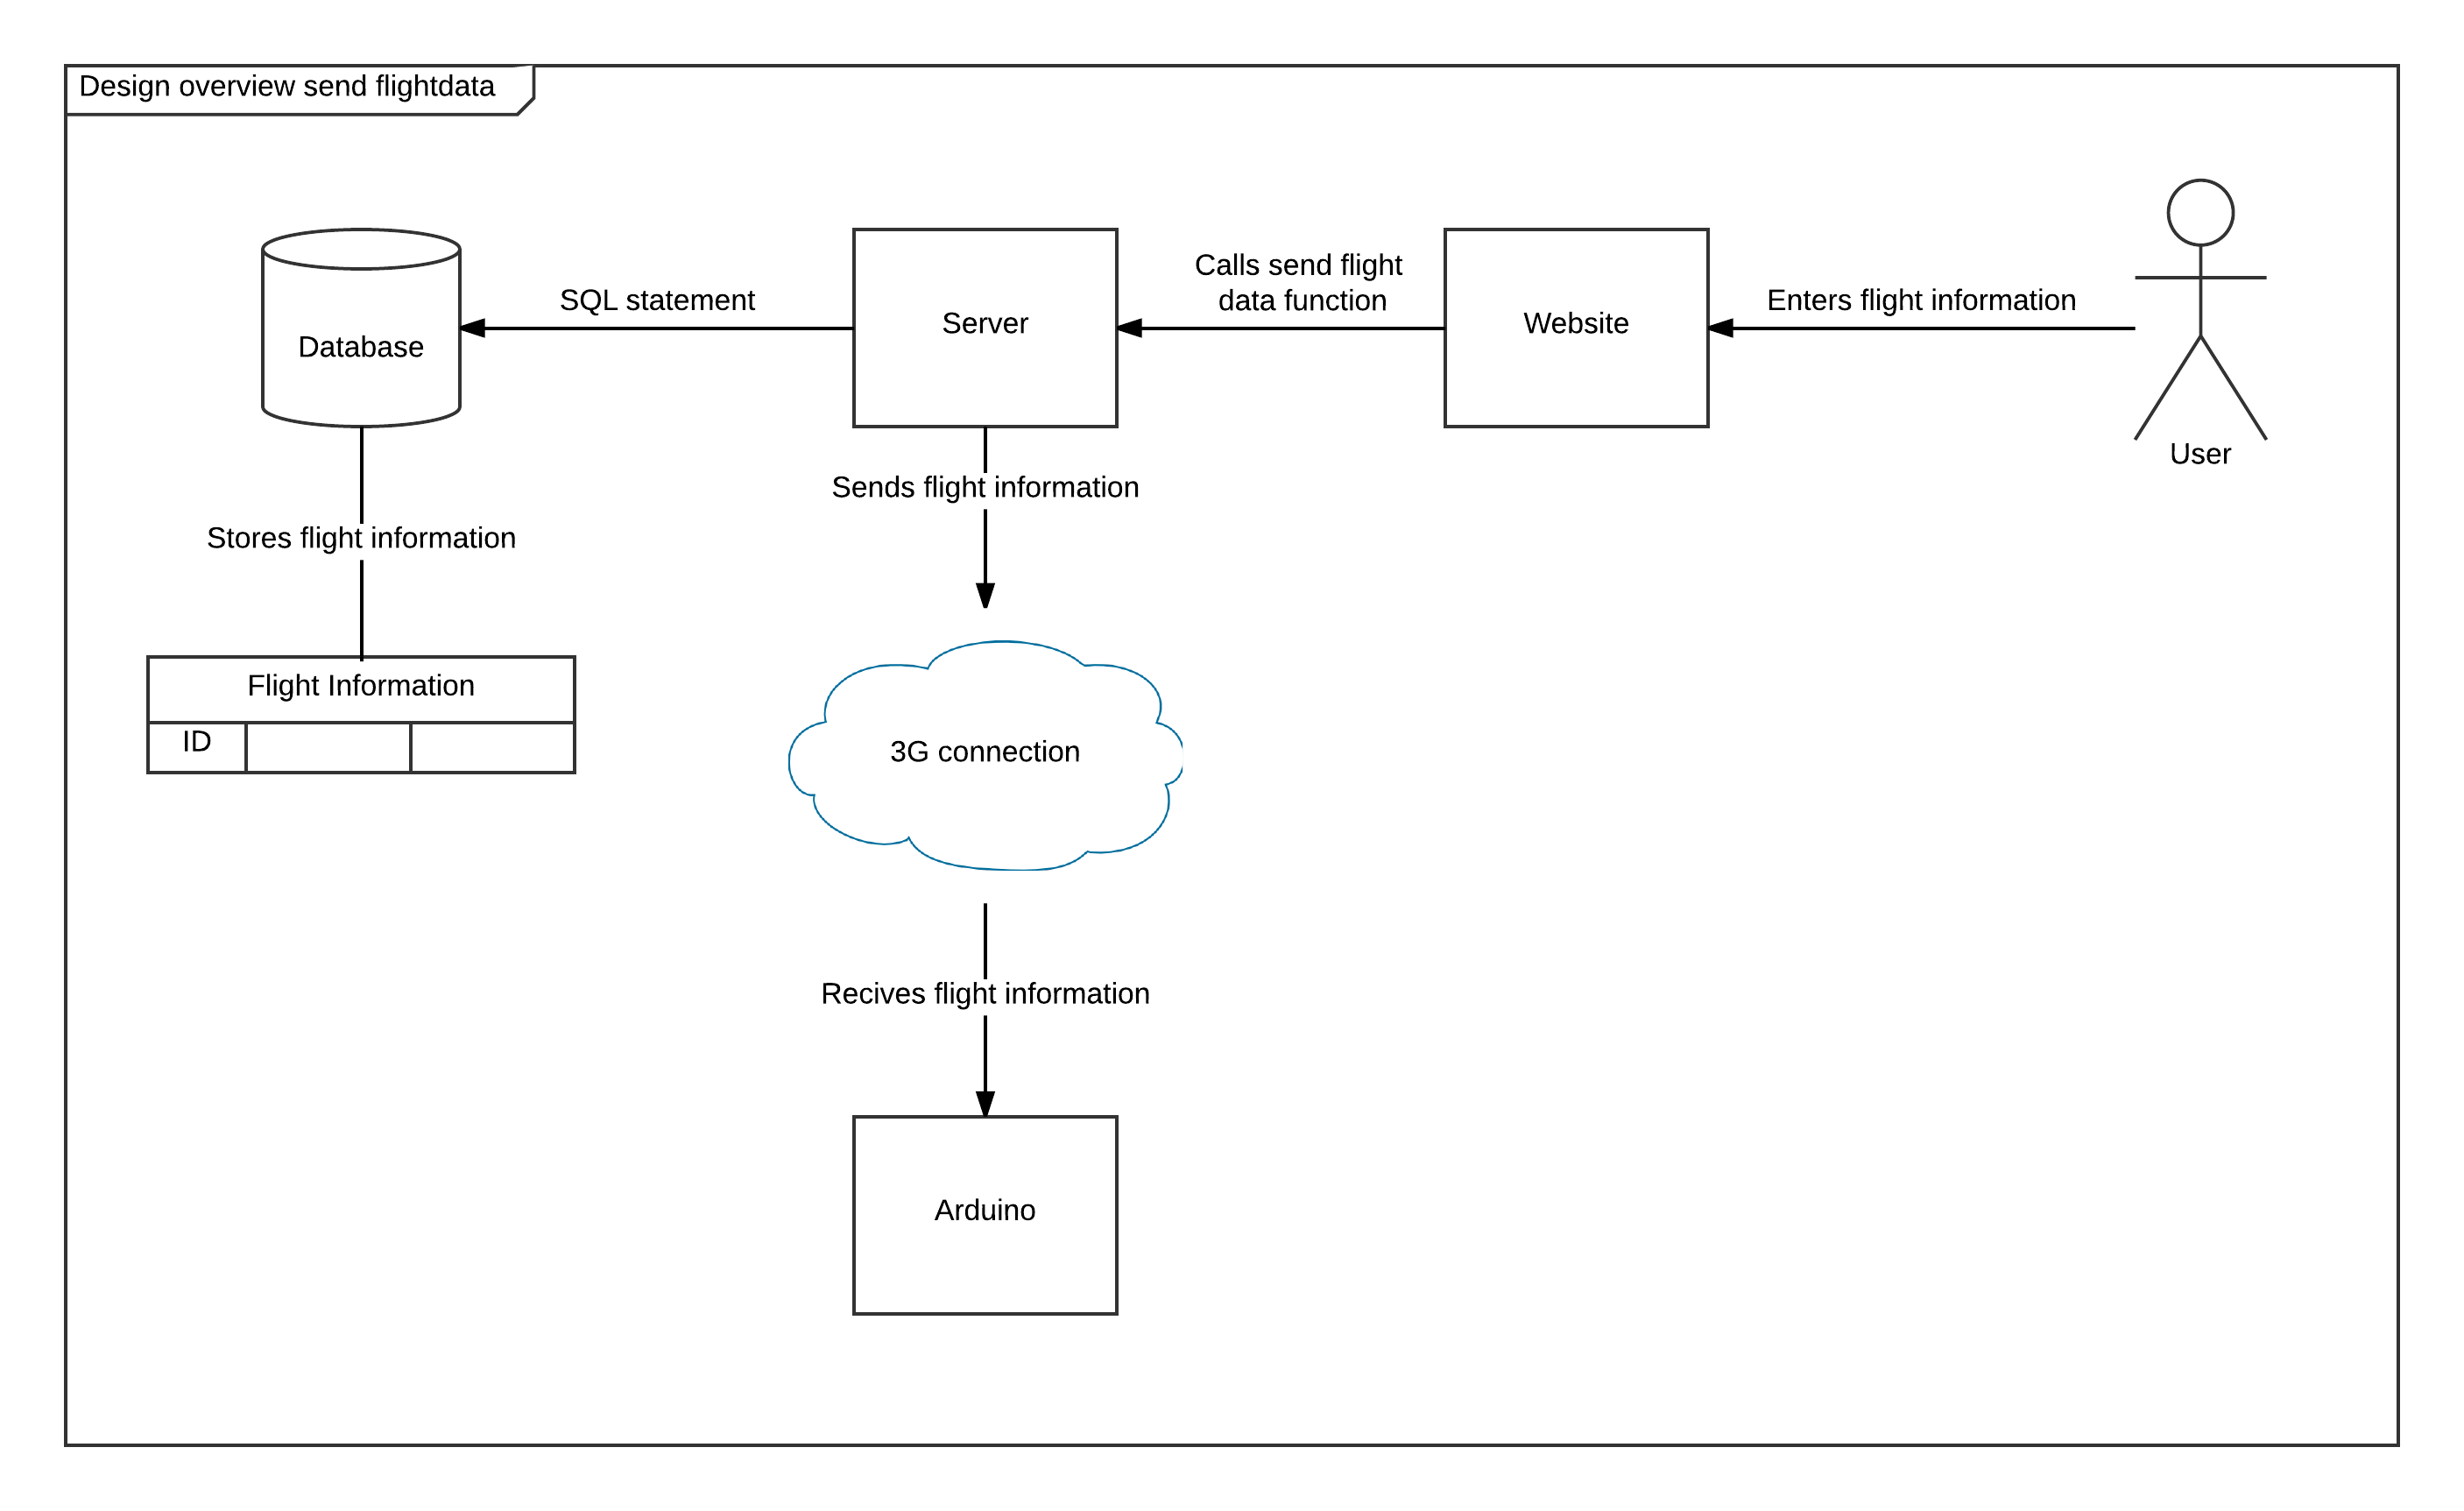
\includegraphics[width=1\textwidth]{Billeder/Design_overview/design_overview_setupFlightdata}
	\vspace{-1cm}
	\caption{Design overview - Setup fligtdata}
	\label{fig:pakke_diagram}
\end{figure}

\newpage
\section{Pakkediagram}

I denne sektion vises pakkediagrammer tilhørende webapplikation og drone. De pakker der vises i pakkediagrammerne består af en eller flere klasser, der med stort samspil udfører opgaver indenfor et fælles ansvarsområde. På hver pakke findes en lille beskrivelse, der tydeliggør pakkens ansvarsområde.

\subsection{Webapplikation}
Figur \ref{fig:pakke_diagram_webapp} viser pakkediagram over webapplikationen. 

\vspace{-5pt}
\begin{figure}[H]
	\centering
	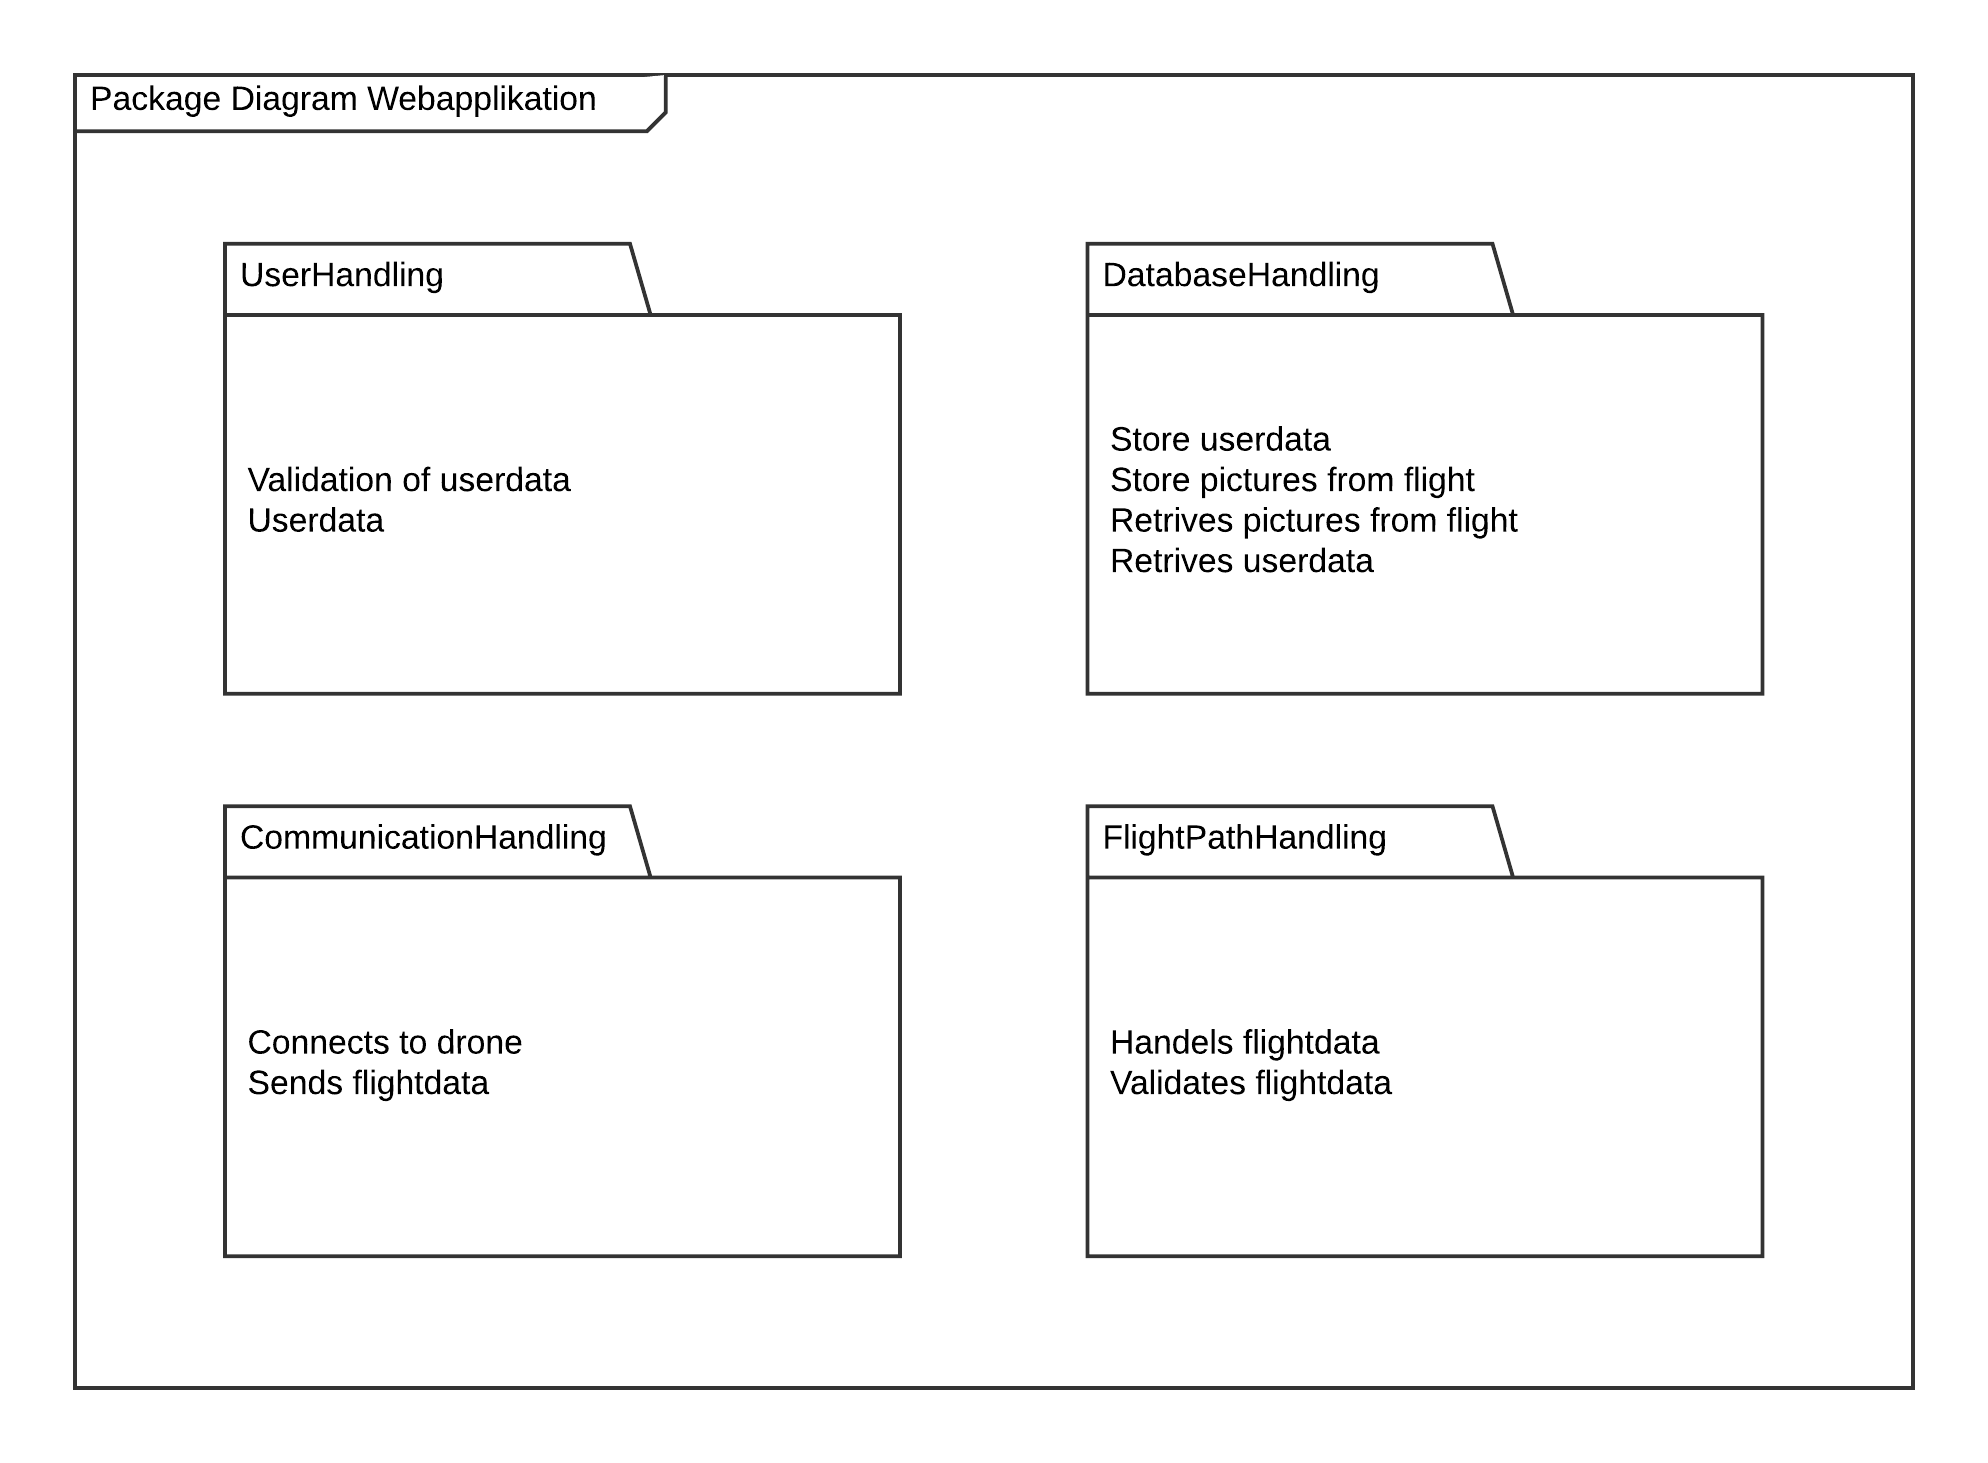
\includegraphics[width=1\textwidth]{Billeder/pakke_diagrammer/package_diagram_webapp.png}
	\vspace{-1cm}
	\caption{Overordnet pakke diagram over webapplikationen}
	\label{fig:pakke_diagram_webapp}
\end{figure}

\textbf{CommunicationHandling}\\
Pakkens ansvar er kommunikation imellem drone og server. Pakken sender flyveinformation til dronen som bruger har lavet på webapplikationen.

\textbf{UserHandling}\\
Pakkens ansvar er validering af login/log ud på websitet. Pakken har også ansvaret for at hente og gemme data om den pågældende bruger.

\textbf{DatabaseHandling}\\
Pakkens ansvar er kommunikation imellem databasen og serveren. 

\textbf{FlightPathHandling}\\
Pakkens ansvar er håndtering af flyveinformation samt validering af dataen.




\newpage
\subsection{Drone}

Figur \ref{fig:pakke_diagram_drone} viser pakkediagram over drone. 

\vspace{-5pt}
\begin{figure}[H]
	\centering
	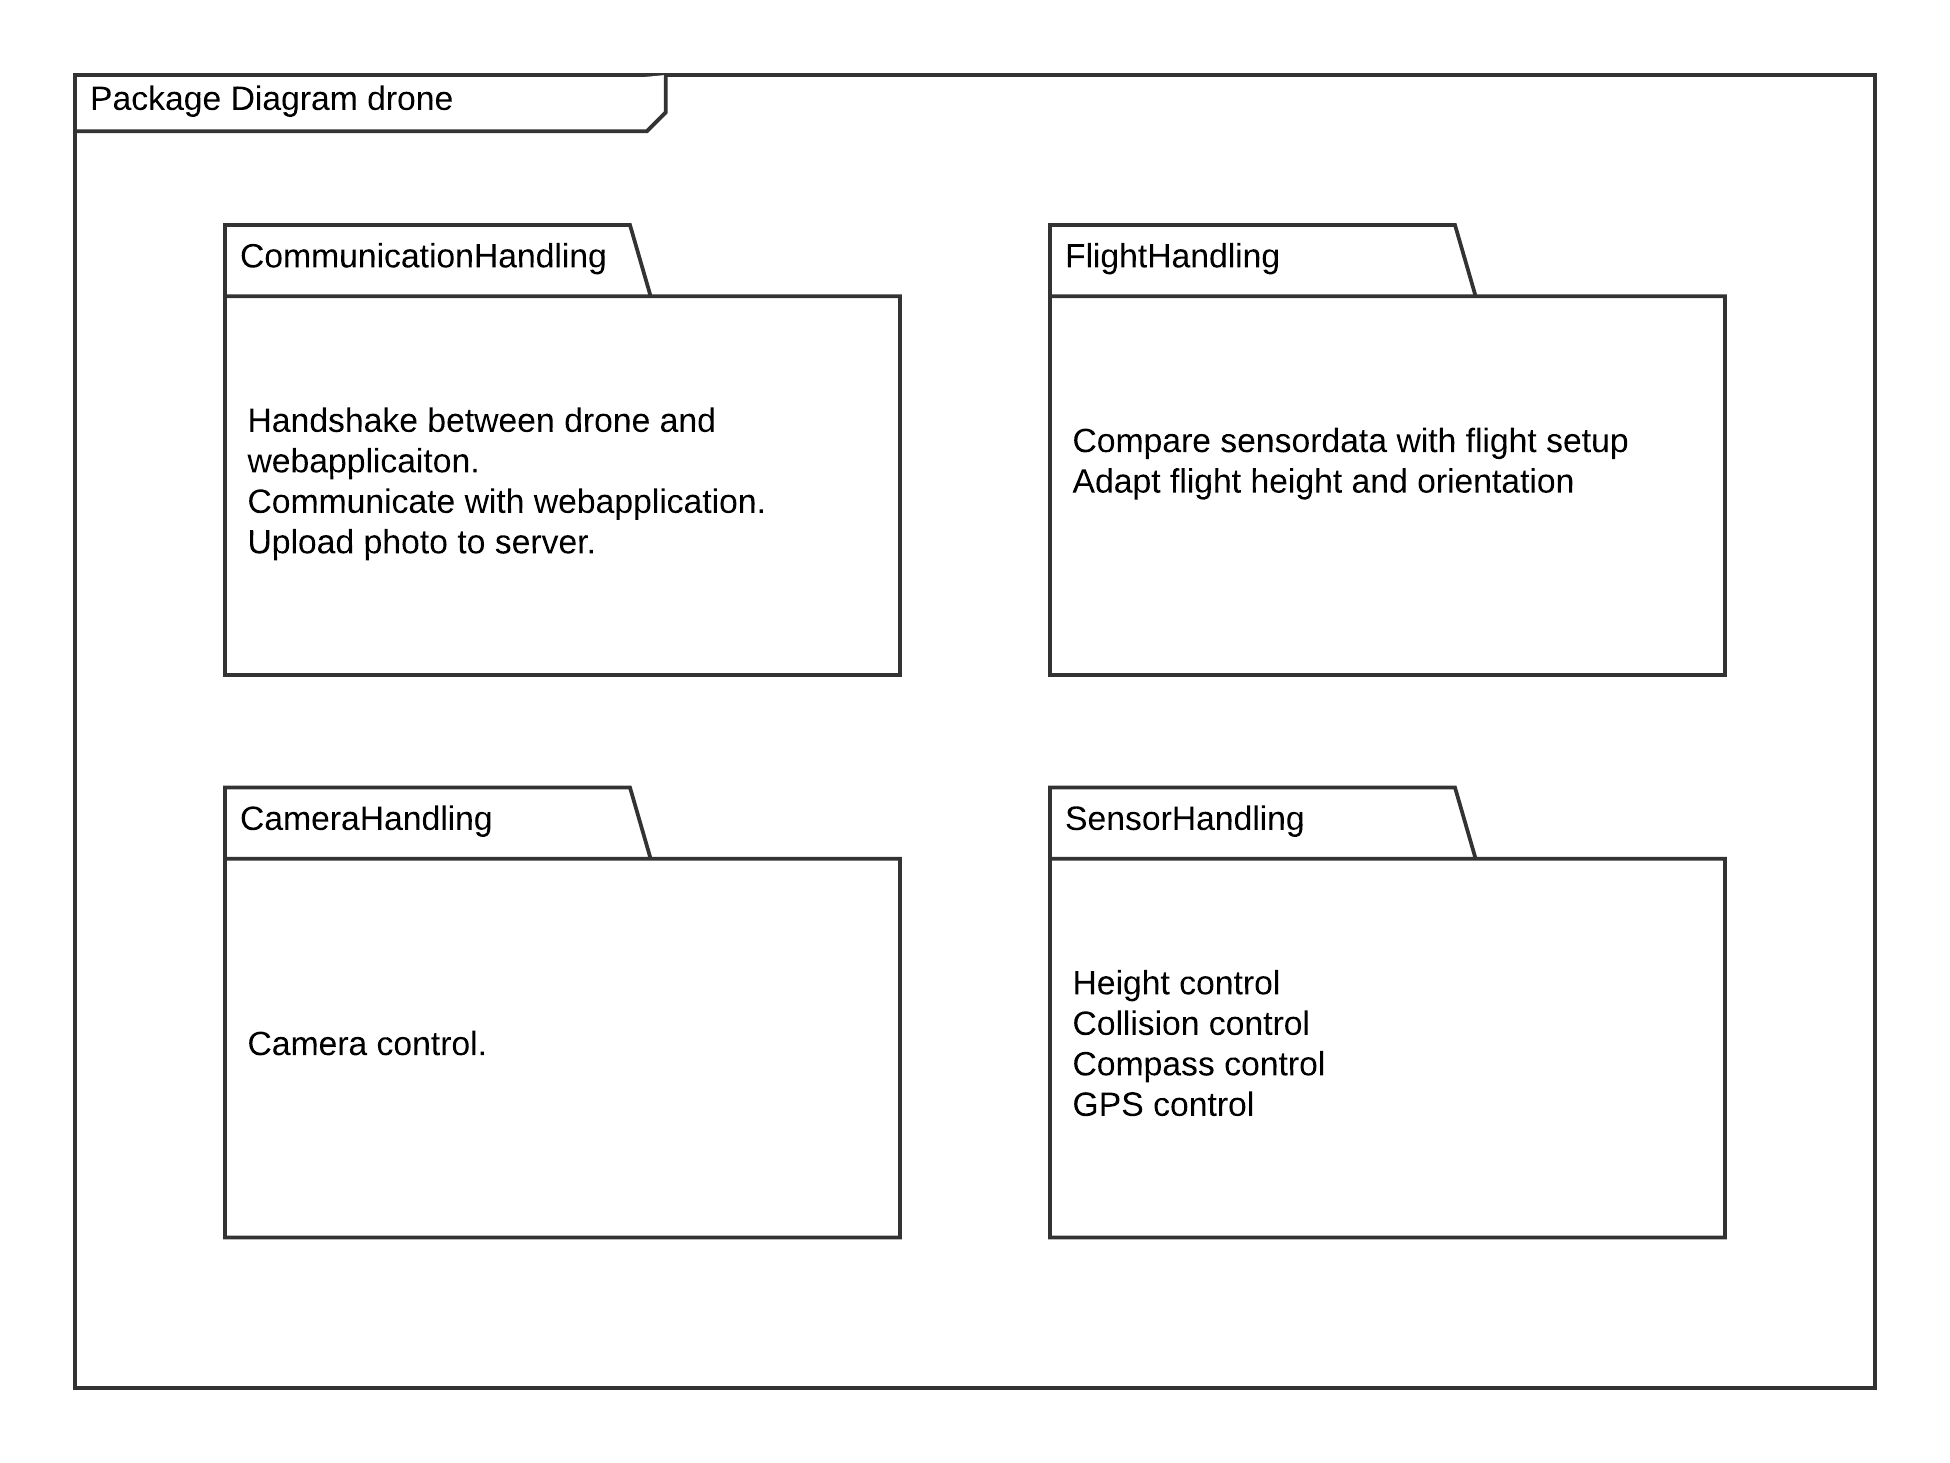
\includegraphics[width=1\textwidth]{Billeder/pakke_diagrammer/package_diagram_drone.png}
	\vspace{-1cm}
	\caption{Overordnet pakke diagram over webapplikationen}
	\label{fig:pakke_diagram_drone}
\end{figure}

\textbf{CommunicationHandling}\\
Pakkens ansvar er kommunikation imellem drone og server. Pakken modtager flyveopsætning som bruger har lavet på webapplikationen og sender billeder til webapplikation.

\textbf{FlightHandling}\\
Pakkens ansvar er at sikre dronen flyver som angivet i flyveopsætning. Pakken har til ansvar at sammenligne data fra sensorer med den modtagne flyveopsætning, og ud fra det regulere dronens flyvehøjde og orientering. 

\textbf{CameraHandling}\\
Pakkens ansvar er håndtering af kamera. Der skal kun tages billeder med kameraet når dronen er på den rette GPS position. 

\textbf{SensorHandling}\\
Pakkens ansvar er håndtering af sensor data.


\newpage
\section{Klasse diagrammer}

\subsection{FlightPathHandling klassediagram}
På klasse diagrammet FlightPathHandling ses de tre overordnet klasser hvilket udgør pakken FlightPathHandling pakken som vist på figur \ref{fig:pakke_diagram}.

\vspace{-5pt}
%kommentar
\begin{figure}[H]
	\centering
	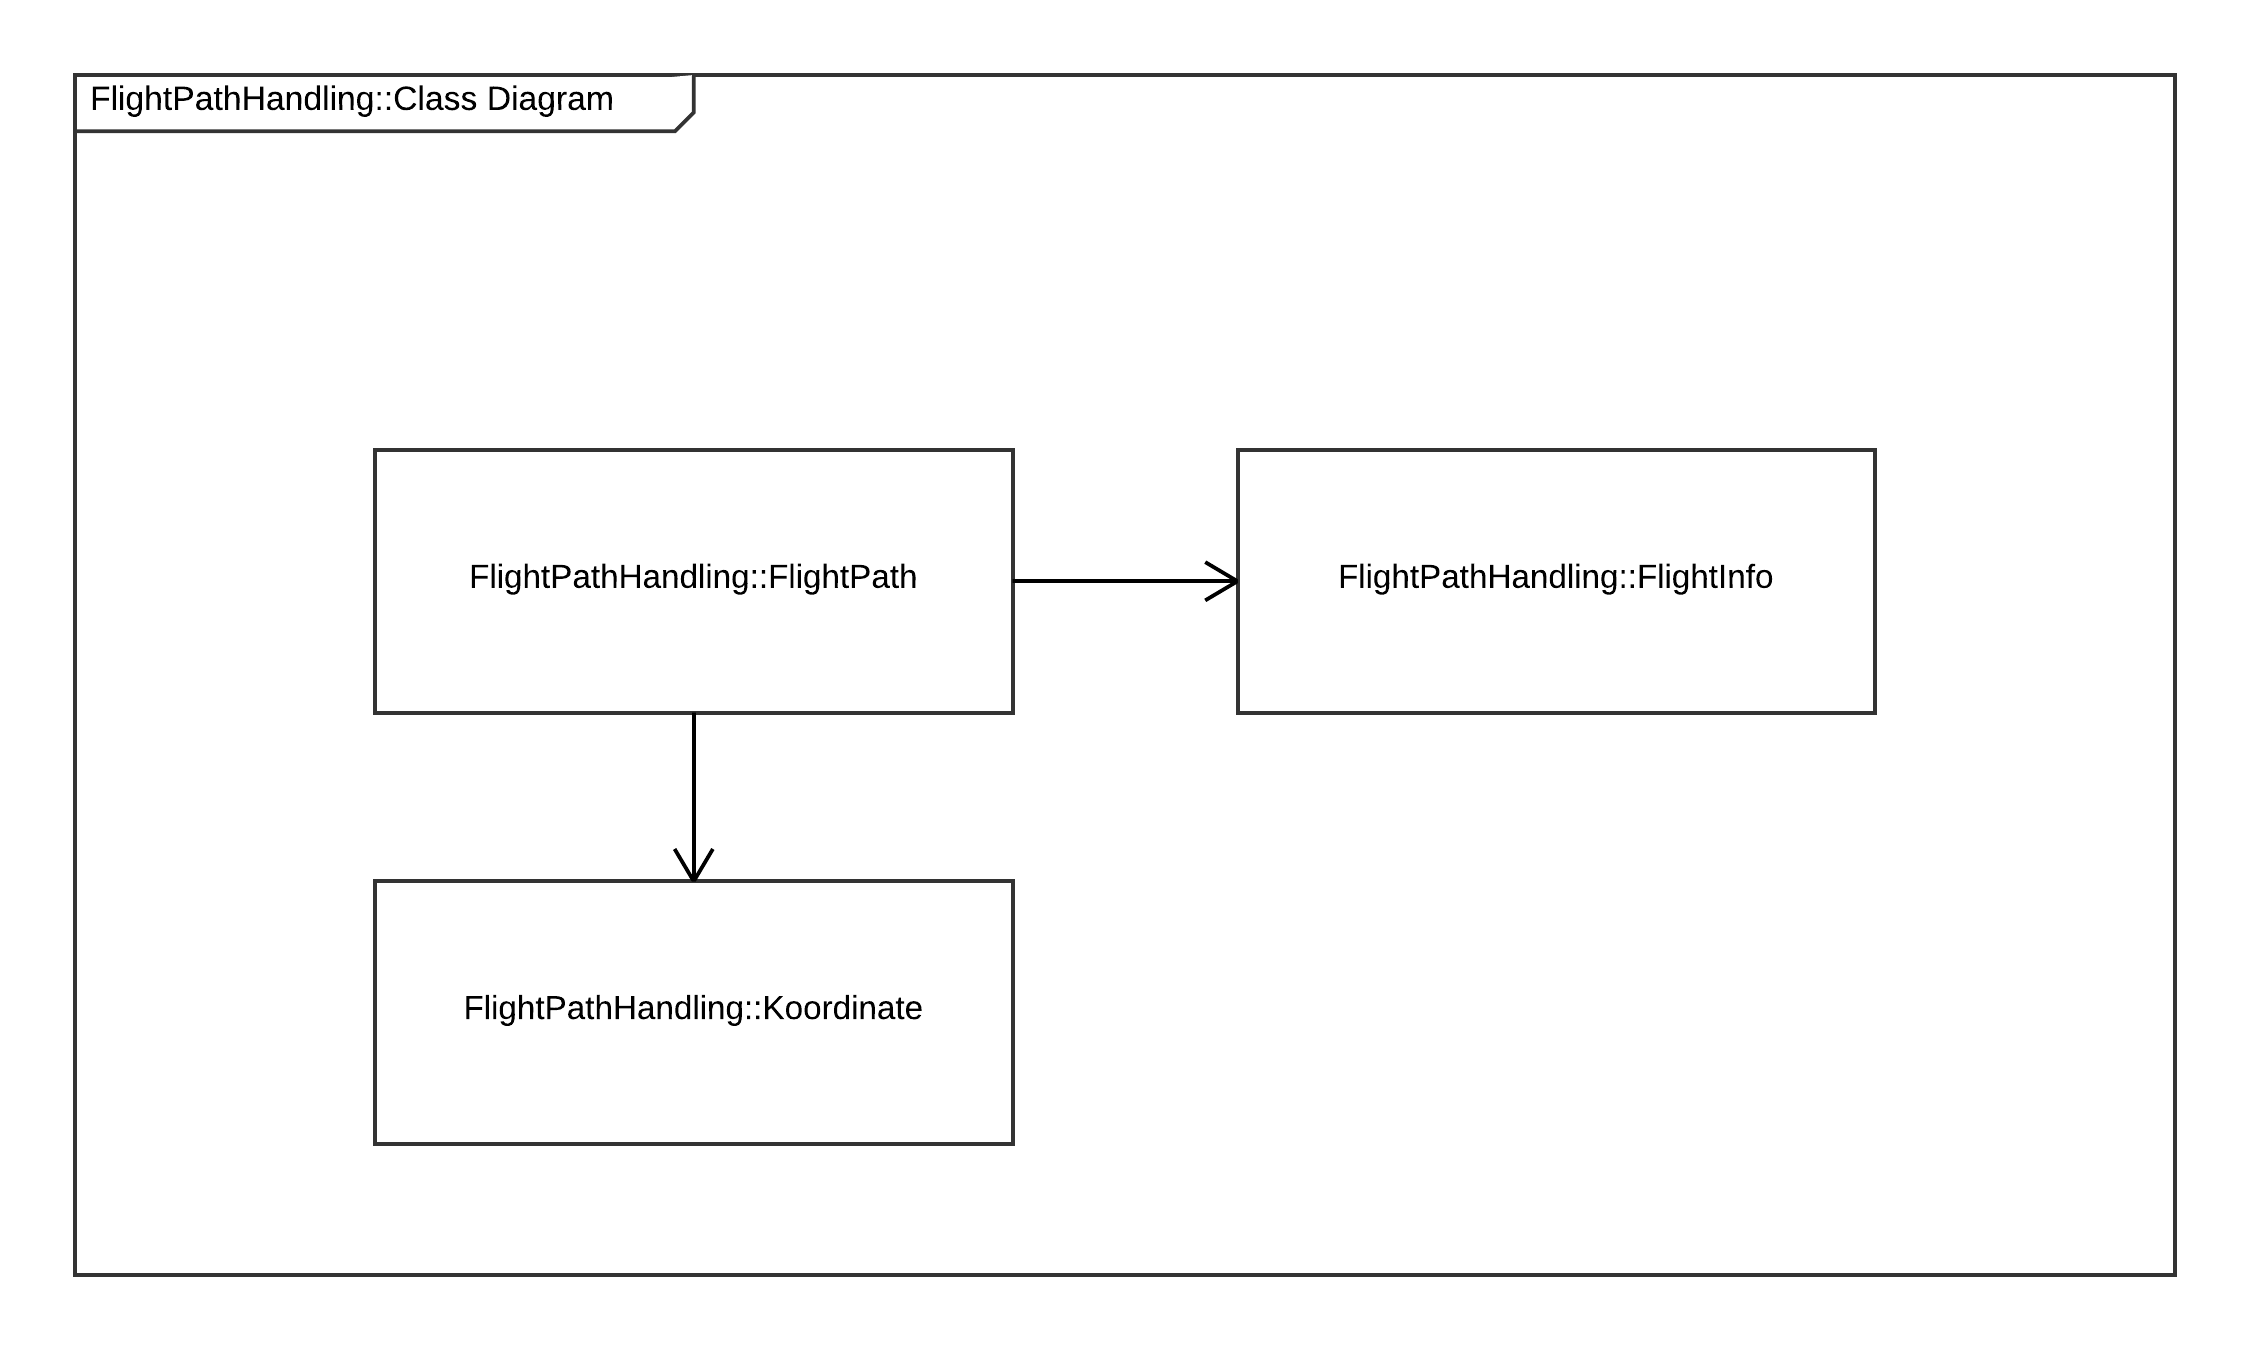
\includegraphics[width=0.7\textwidth]{Billeder/klasse_diagrammer/FlightPathHandlingDiagram.png}
	\vspace{-5pt}
	\caption{FlightPathHandling klasse diagram}
	\label{fig:FlightPathHandling_klasse_diagram}
\end{figure}

\textbf{FlightPath}\\
Klassen FlightPath bruger både FlightInfo og Coordinate klasserne til at udgøre en FlightPath.

\textbf{Coordinate}\\
Coordinate klassen håndtere det GPS koordinater som brugeren ønsker dronen skal flyve til.

\textbf{FlightInfo}\\
FlightInfo klassen håndtere data om ruten så som flyvehøjde, dato for flyvning.

\textbf{FileHandling}\\
FileHandling klassen genere en fil ud fra data'en i FlightPath som så sendes til dronen.

\textbf{JSONFormat}\\
Klassen nedarver fra FileHandling for at kunne bruges som FileHandling. Klassen genere en JSON fil som kan sendes til dronen.

\newpage
\subsection{UserHandling}
Klasse diagrammet viser hvilket klasser som udgør UserHandling pakken som vist på figur \ref{fig:pakke_diagram}.

\vspace{-5pt}
%kommentar
\begin{figure}[H]
	\centering
	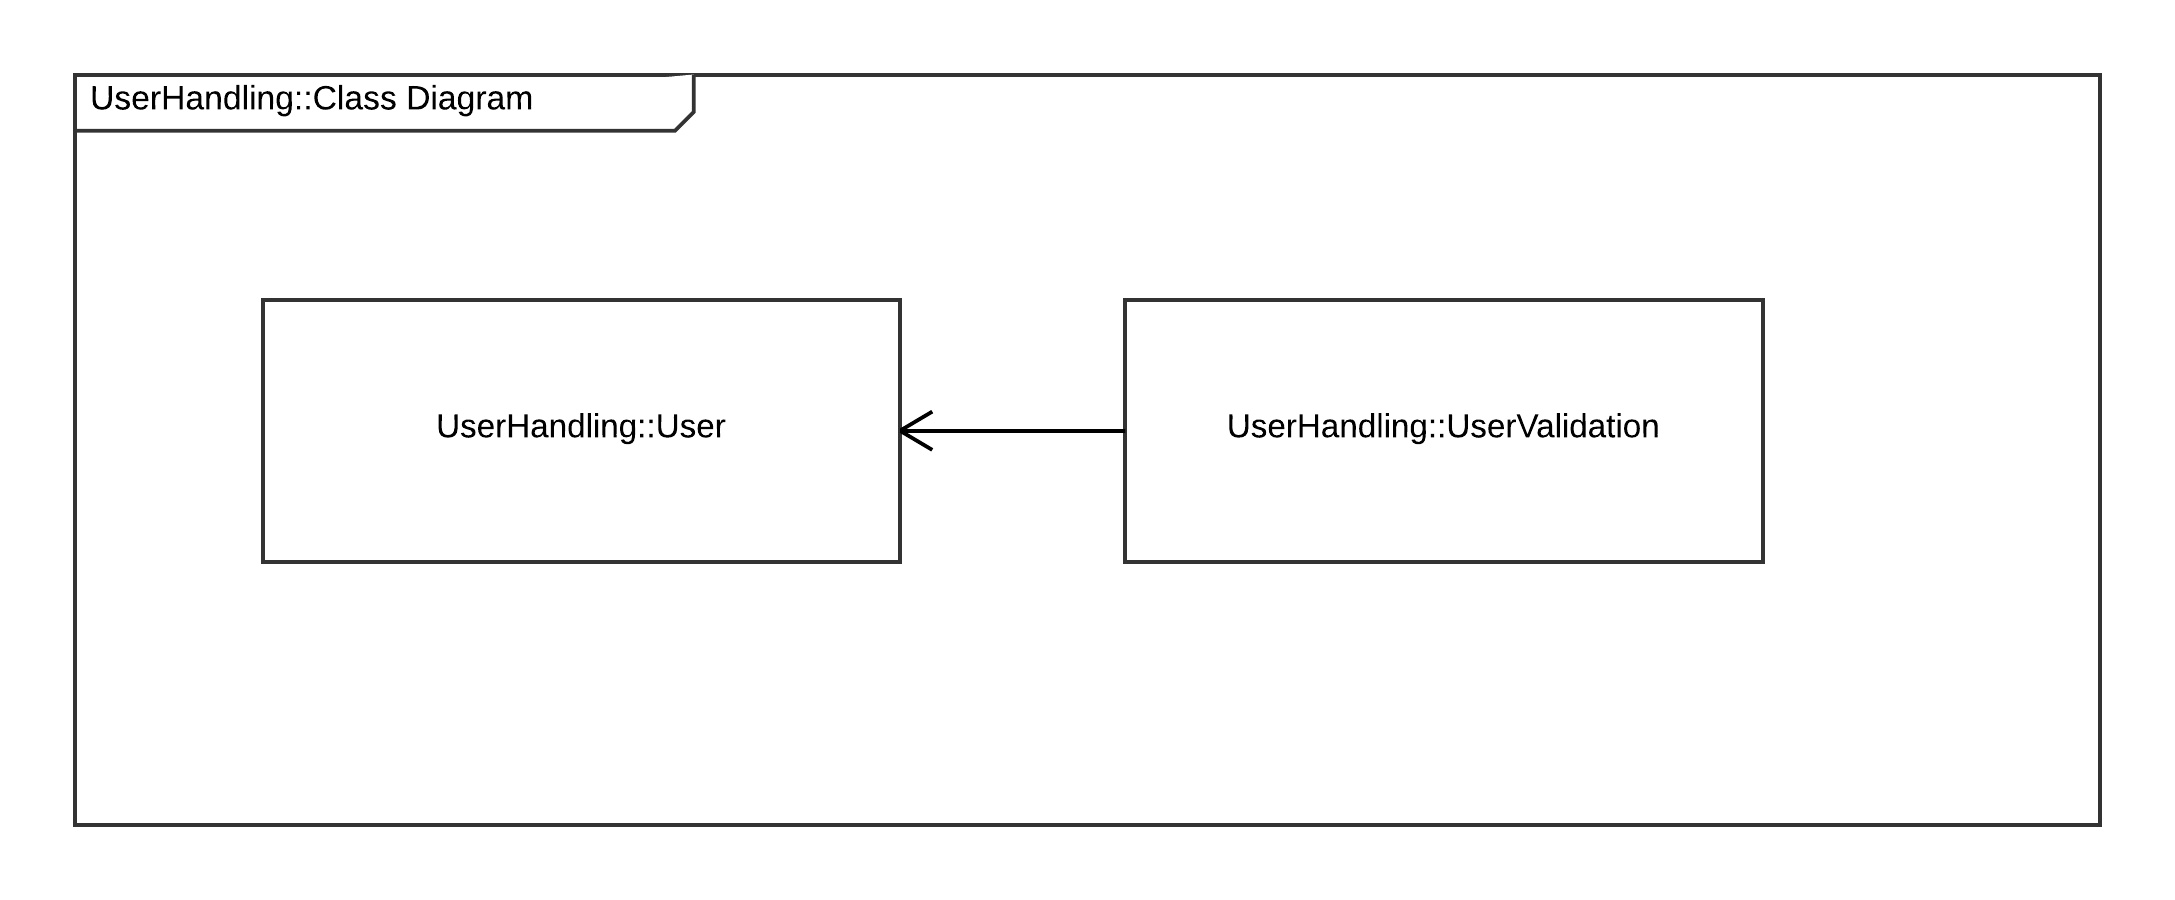
\includegraphics[width=0.7\textwidth]{Billeder/klasse_diagrammer/UserHandlingDiagram.png}
	\vspace{-5pt}
	\caption{UserHandling klasse diagram}
	\label{fig:UserHandling_klasse_diagram}
\end{figure}

\textbf{User}\\
User klassen indeholder alle data om brugerne i systemet. Klassen bliver også brugt af UserValidation i forbindelse med login/log out.

\textbf{UserValidation}\\
UserValidation klassen har ansvaret for at validere en user når der bliver forsøgt login.\\

\newpage
\subsection{DatabaseHandling}
Klasse diagrammet viser hvilket klasser som udgør DatabaseHandling pakken som vist på figur \ref{fig:pakke_diagram}.

\vspace{-5pt}
%kommentar
\begin{figure}[H]
	\centering
	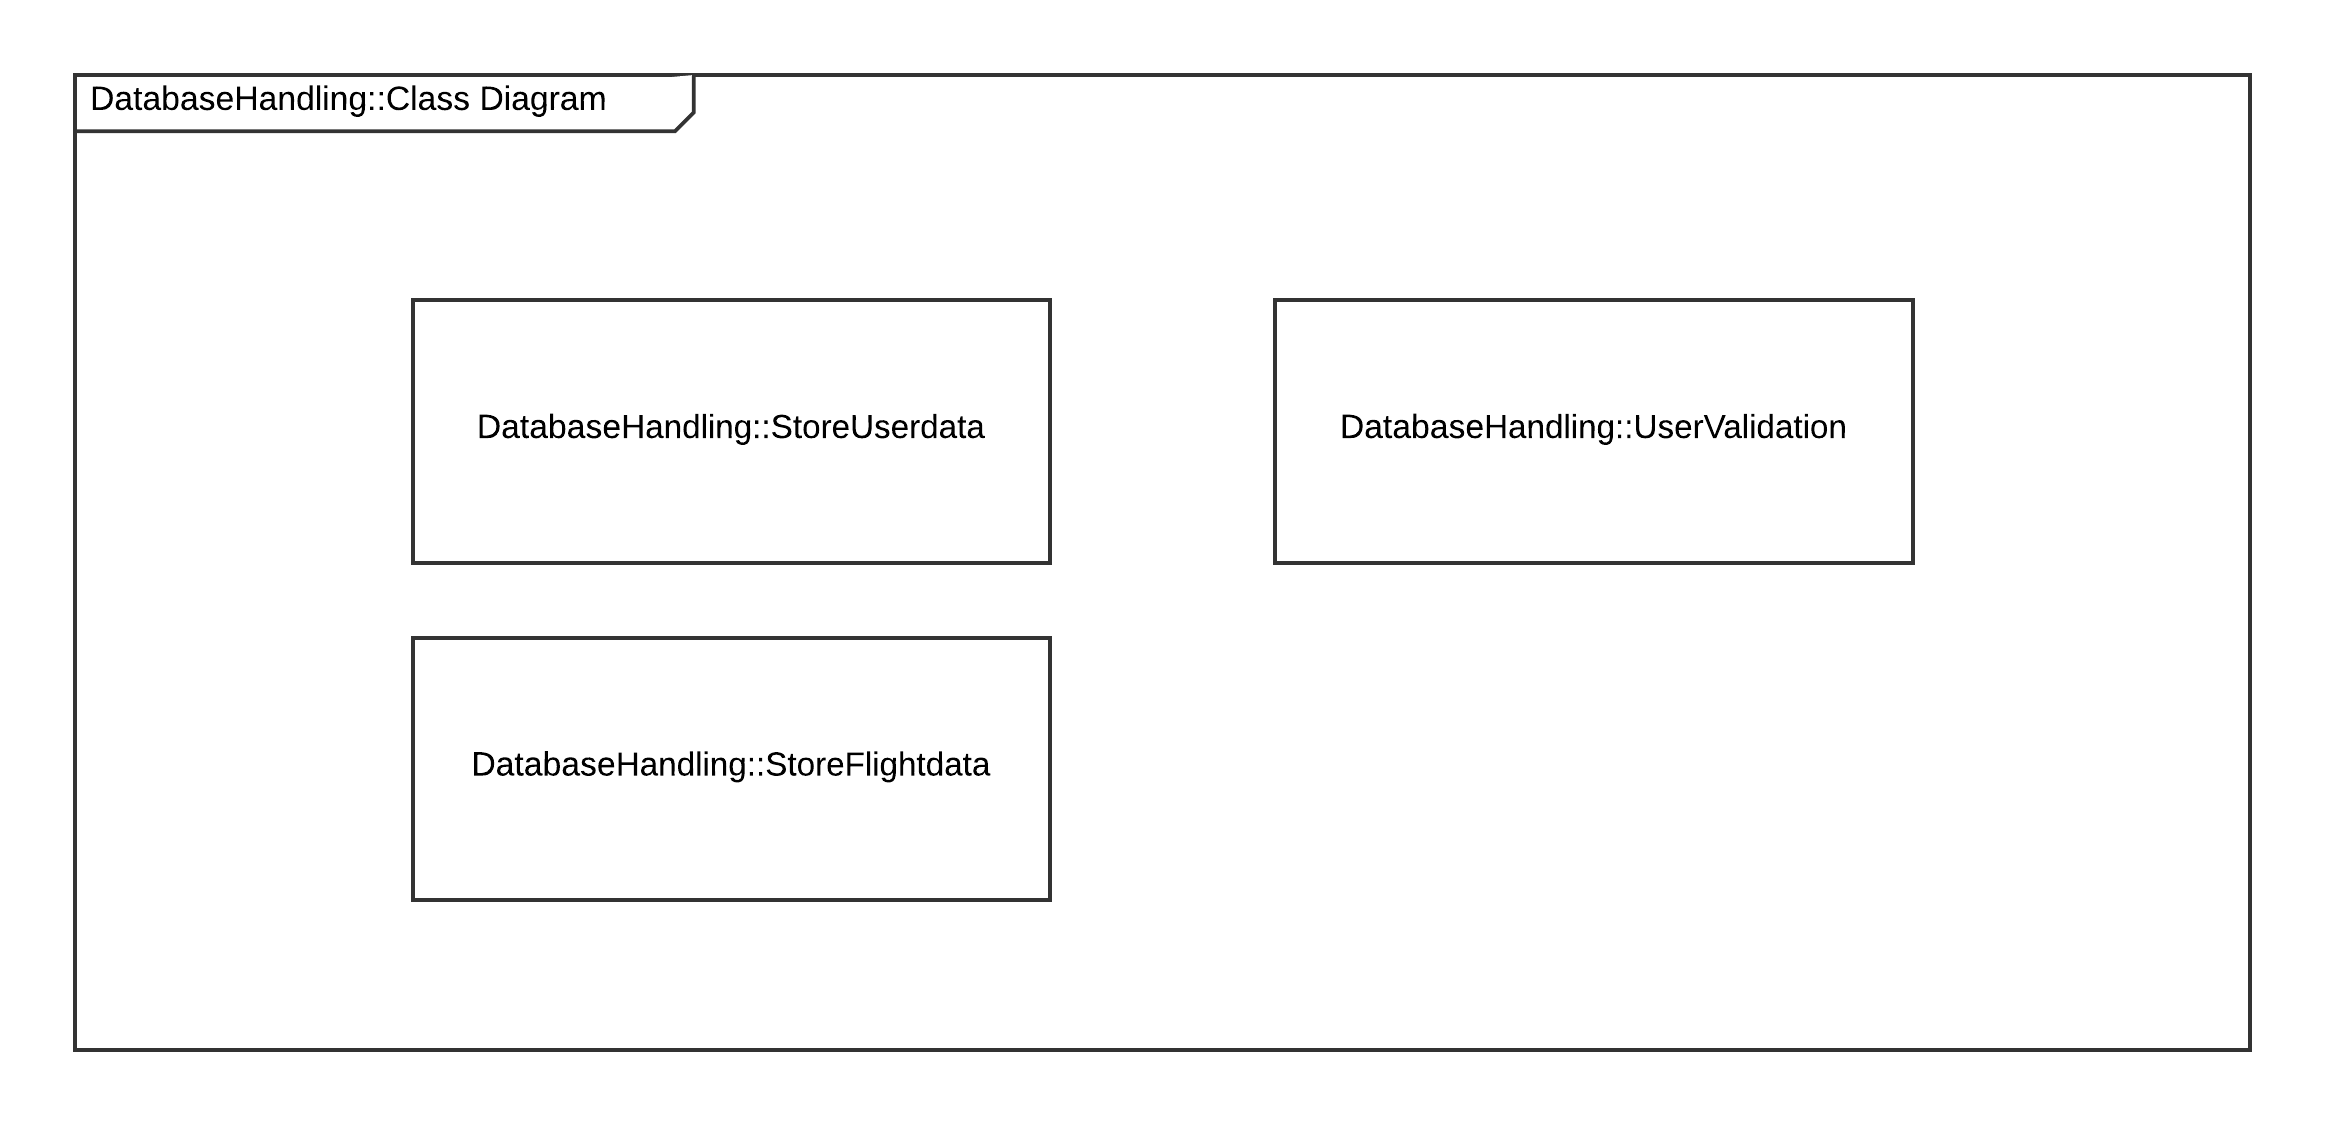
\includegraphics[width=0.7\textwidth]{Billeder/klasse_diagrammer/DatabaseHandling.png}
	\vspace{-5pt}
	\caption{DatabaseHandling klasse diagram}
	\label{fig:DatabaseHandling_klasse_diagram}
\end{figure}

\textbf{DatabaseConnection}\\
Superklassen DatabaseConnection har til ansvar at skabe forbindelse til databasen og lukke kommunikationen ned efter data overførelse. De andre klasser nedarver fra klassen så de kan oprette forbindelse og lukke forbindelsen.

\textbf{StoreUserdata}\\
Klassen opdatere brugerdata i databasen. Igennem nedarvningen fra superklassen DatabaseConnection kan StoreUserdata også oprette forbindelse og lukke forbindelsen igen til databasen.

\textbf{StoreFlightdata}\\
StoreFlightdata gemmer alle data omkring flyvning. Denne klasse bruges løbende under flyvning når billeder bliver modtaget og skal gemmes til en igangværende flyvning.

\textbf{UserValidation}\\
UserValidation validaere bruger ved forsøg på login og giver adgang til systemet hvis brugeren er valid.

\newpage
\subsection{CommunicationHandling}
Klasse diagrammet viser hvilket klasser som udgør CommunicationHandling pakken som vist på figur \ref{fig:pakke_diagram}.

\vspace{-5pt}
%kommentar
\begin{figure}[H]
	\centering
	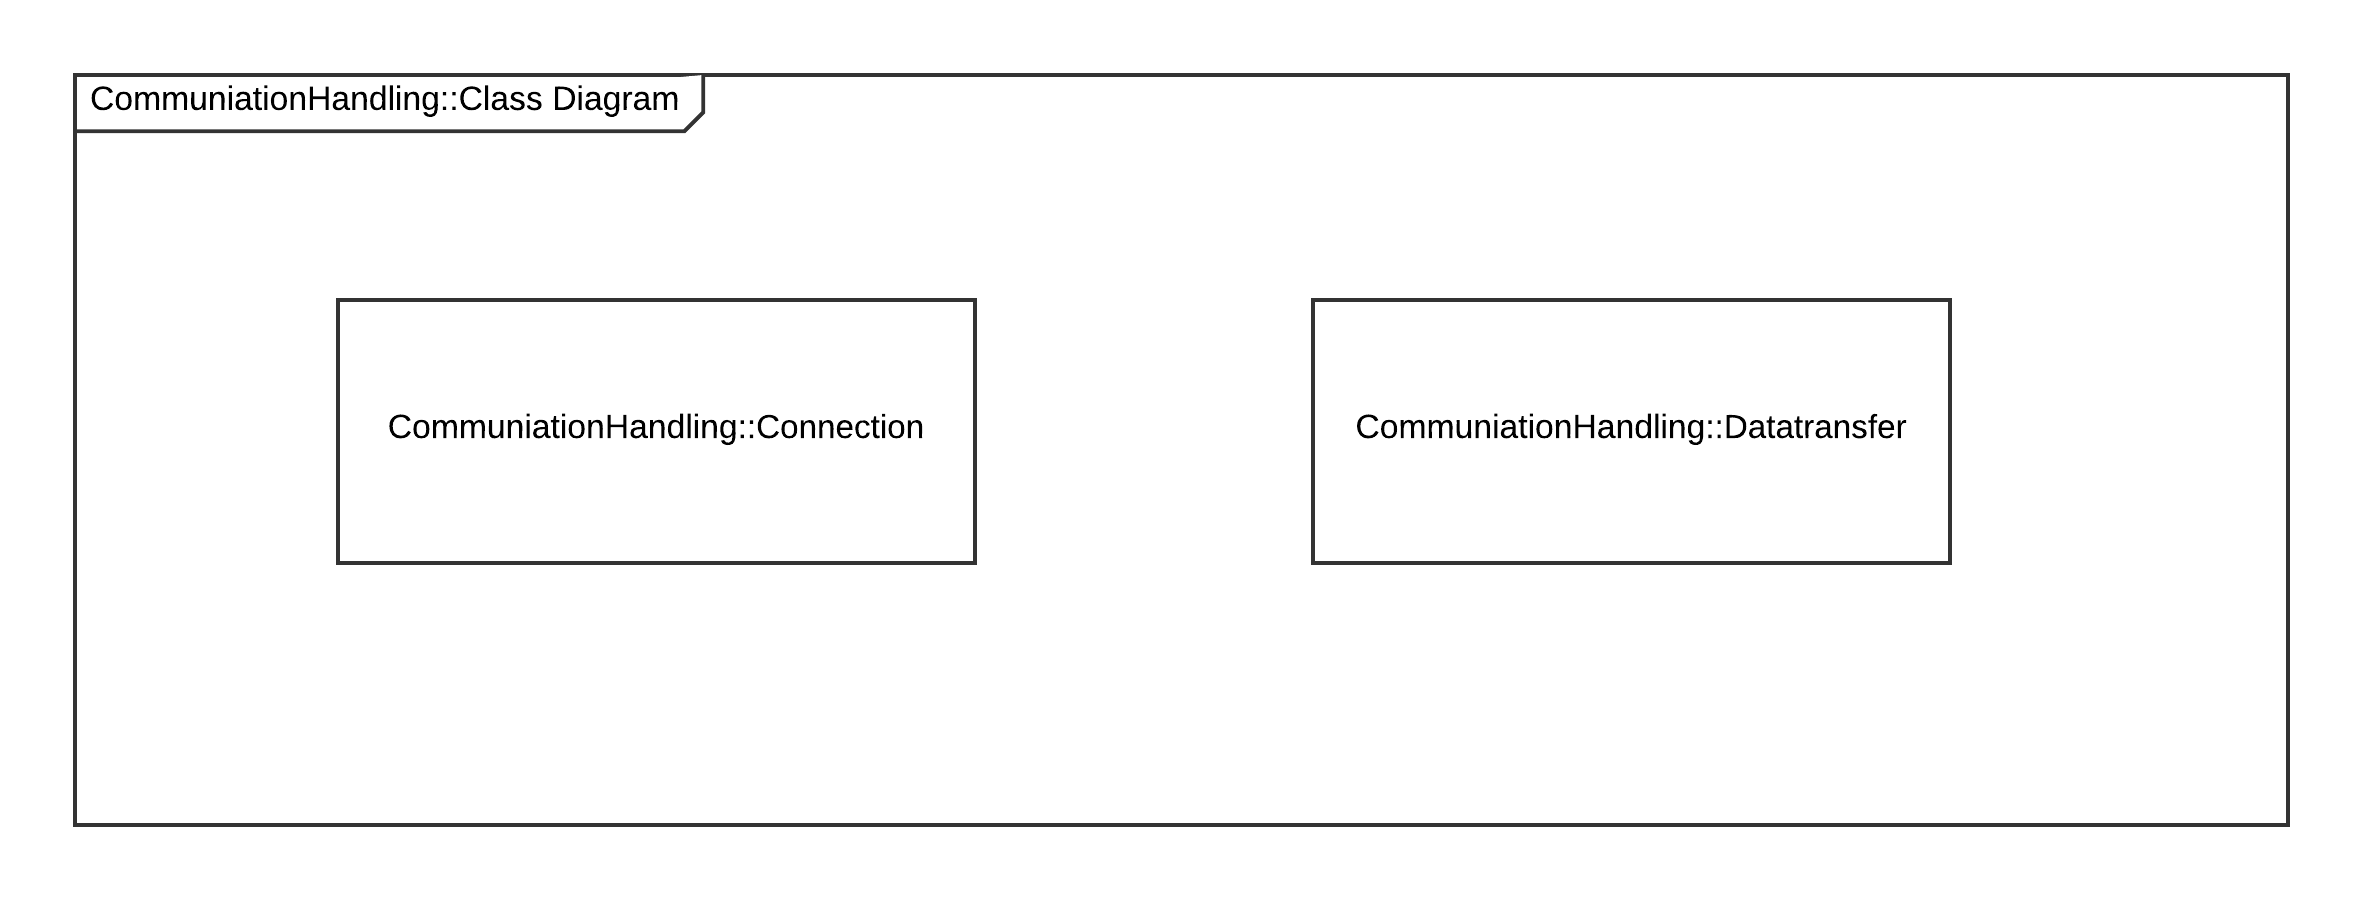
\includegraphics[width=0.7\textwidth]{Billeder/klasse_diagrammer/CommunicationHandling.png}
	\vspace{-5pt}
	\caption{CommunicationHandling klasse diagram}
	\label{fig:CommunicationHandling_klasse_diagram}
\end{figure}

\textbf{Connection}\\
Connection klassen har til ansvar for at skabe forbindelse imellem serveren og dronen.

\textbf{Datatransfer}\\
Datatransfer klassen bruger connection klassen til at oprette forbindelse til dronen inden data'en sendes. 


%\newpage
%\section{Pakkediagram}

I denne sektion vises pakkediagrammer tilhørende webapplikation og drone. De pakker der vises i pakkediagrammerne består af en eller flere klasser, der med stort samspil udfører opgaver indenfor et fælles ansvarsområde. På hver pakke findes en lille beskrivelse, der tydeliggør pakkens ansvarsområde.

\subsection{Webapplikation}
Figur \ref{fig:pakke_diagram_webapp} viser pakkediagram over webapplikationen. 

\vspace{-5pt}
\begin{figure}[H]
	\centering
	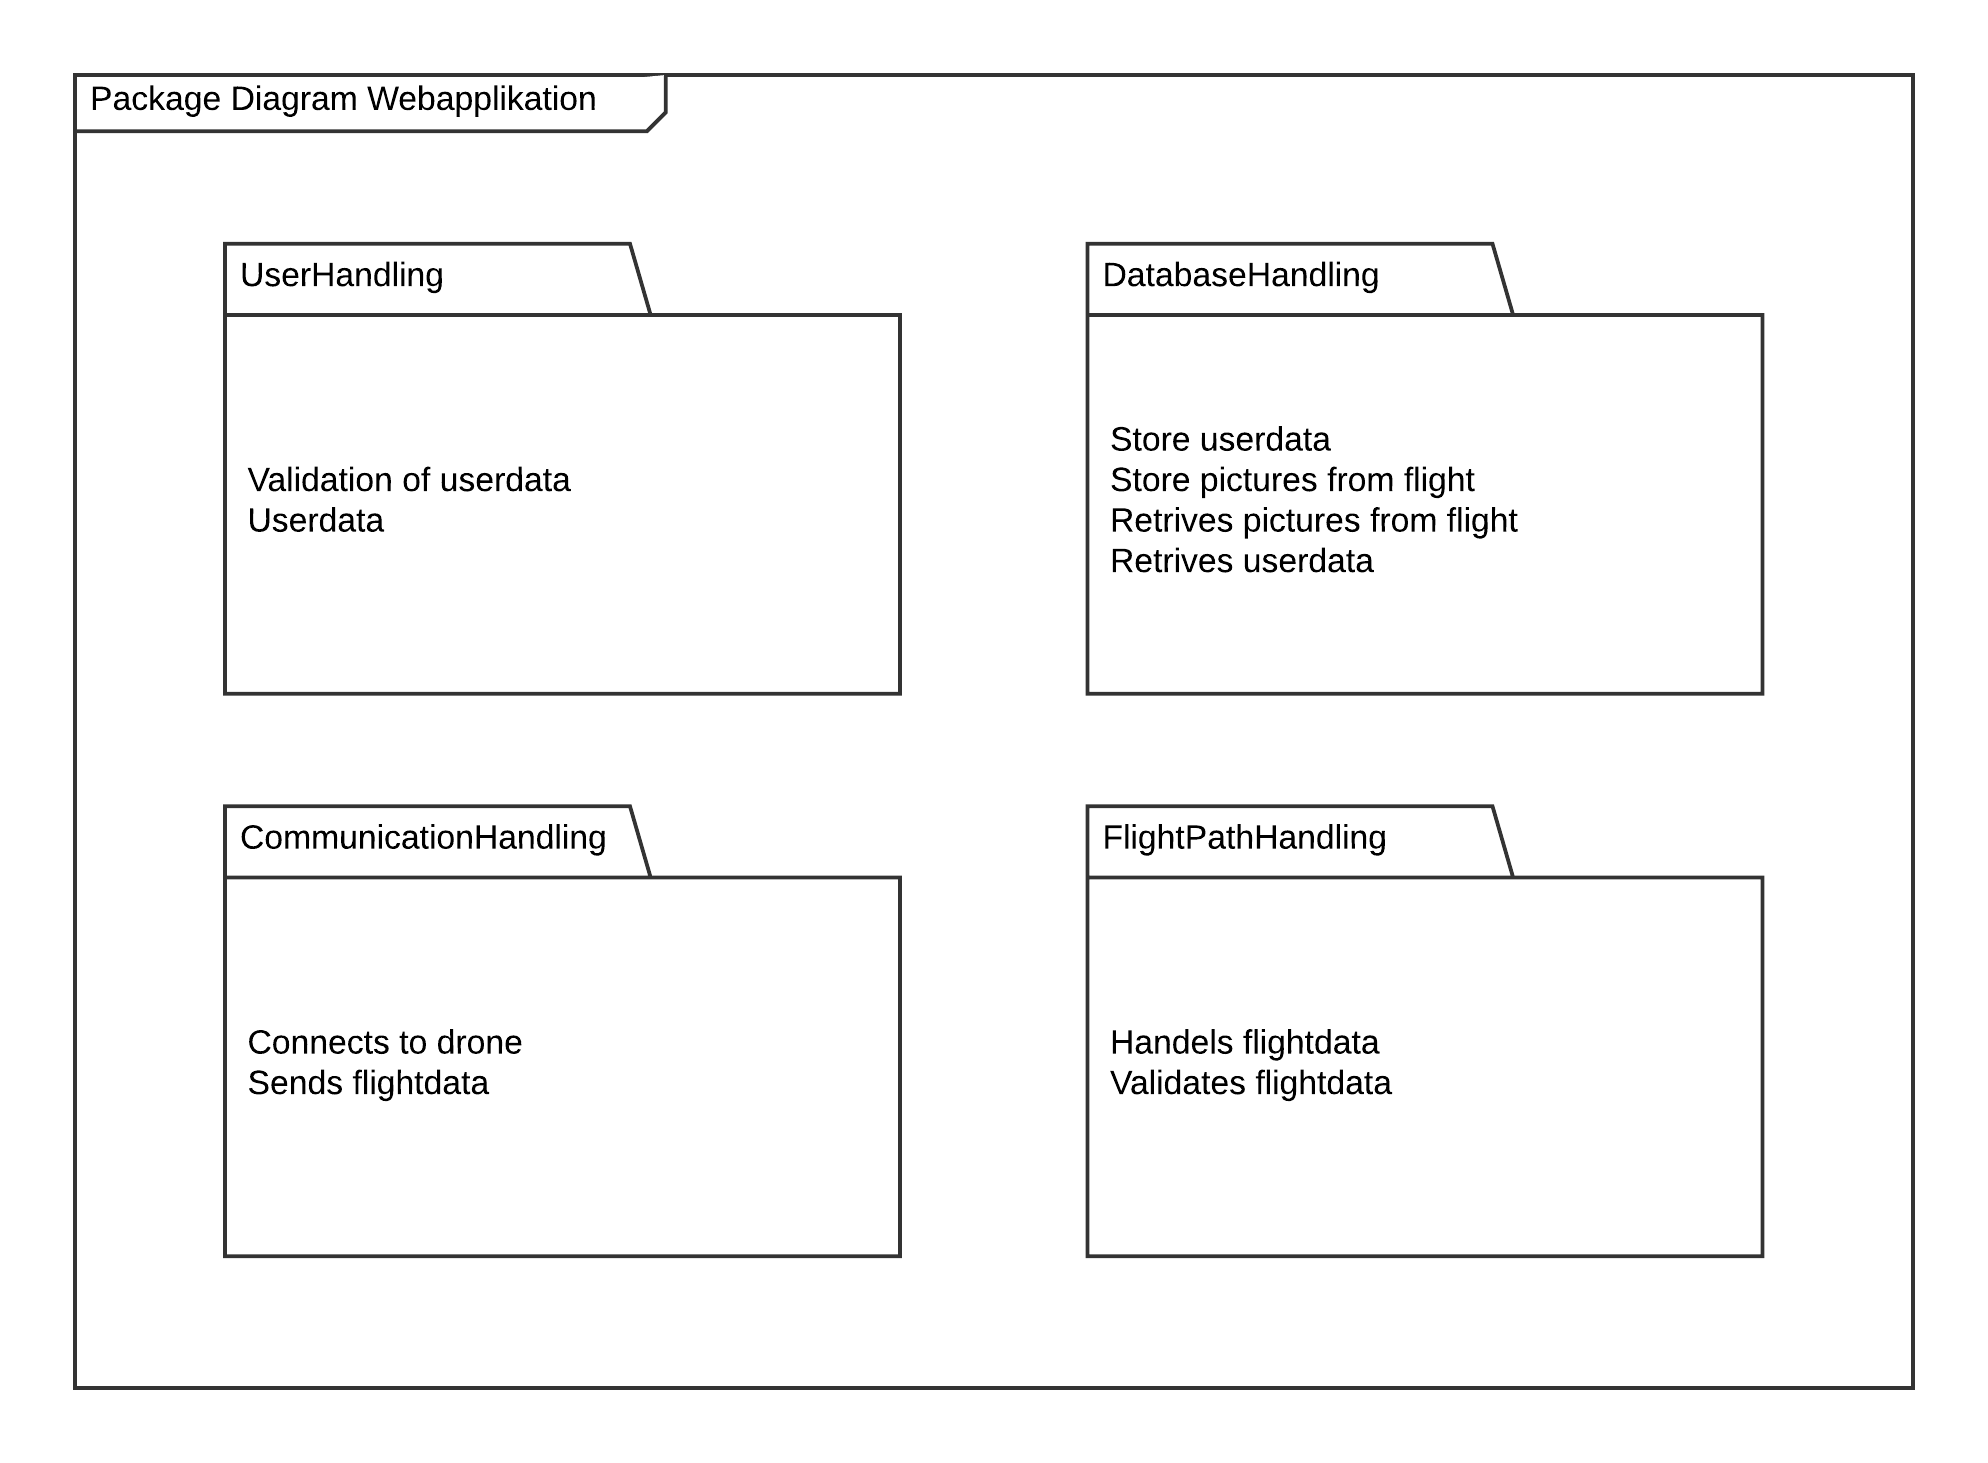
\includegraphics[width=1\textwidth]{Billeder/pakke_diagrammer/package_diagram_webapp.png}
	\vspace{-1cm}
	\caption{Overordnet pakke diagram over webapplikationen}
	\label{fig:pakke_diagram_webapp}
\end{figure}

\textbf{CommunicationHandling}\\
Pakkens ansvar er kommunikation imellem drone og server. Pakken sender flyveinformation til dronen som bruger har lavet på webapplikationen.

\textbf{UserHandling}\\
Pakkens ansvar er validering af login/log ud på websitet. Pakken har også ansvaret for at hente og gemme data om den pågældende bruger.

\textbf{DatabaseHandling}\\
Pakkens ansvar er kommunikation imellem databasen og serveren. 

\textbf{FlightPathHandling}\\
Pakkens ansvar er håndtering af flyveinformation samt validering af dataen.




\newpage
\subsection{Drone}

Figur \ref{fig:pakke_diagram_drone} viser pakkediagram over drone. 

\vspace{-5pt}
\begin{figure}[H]
	\centering
	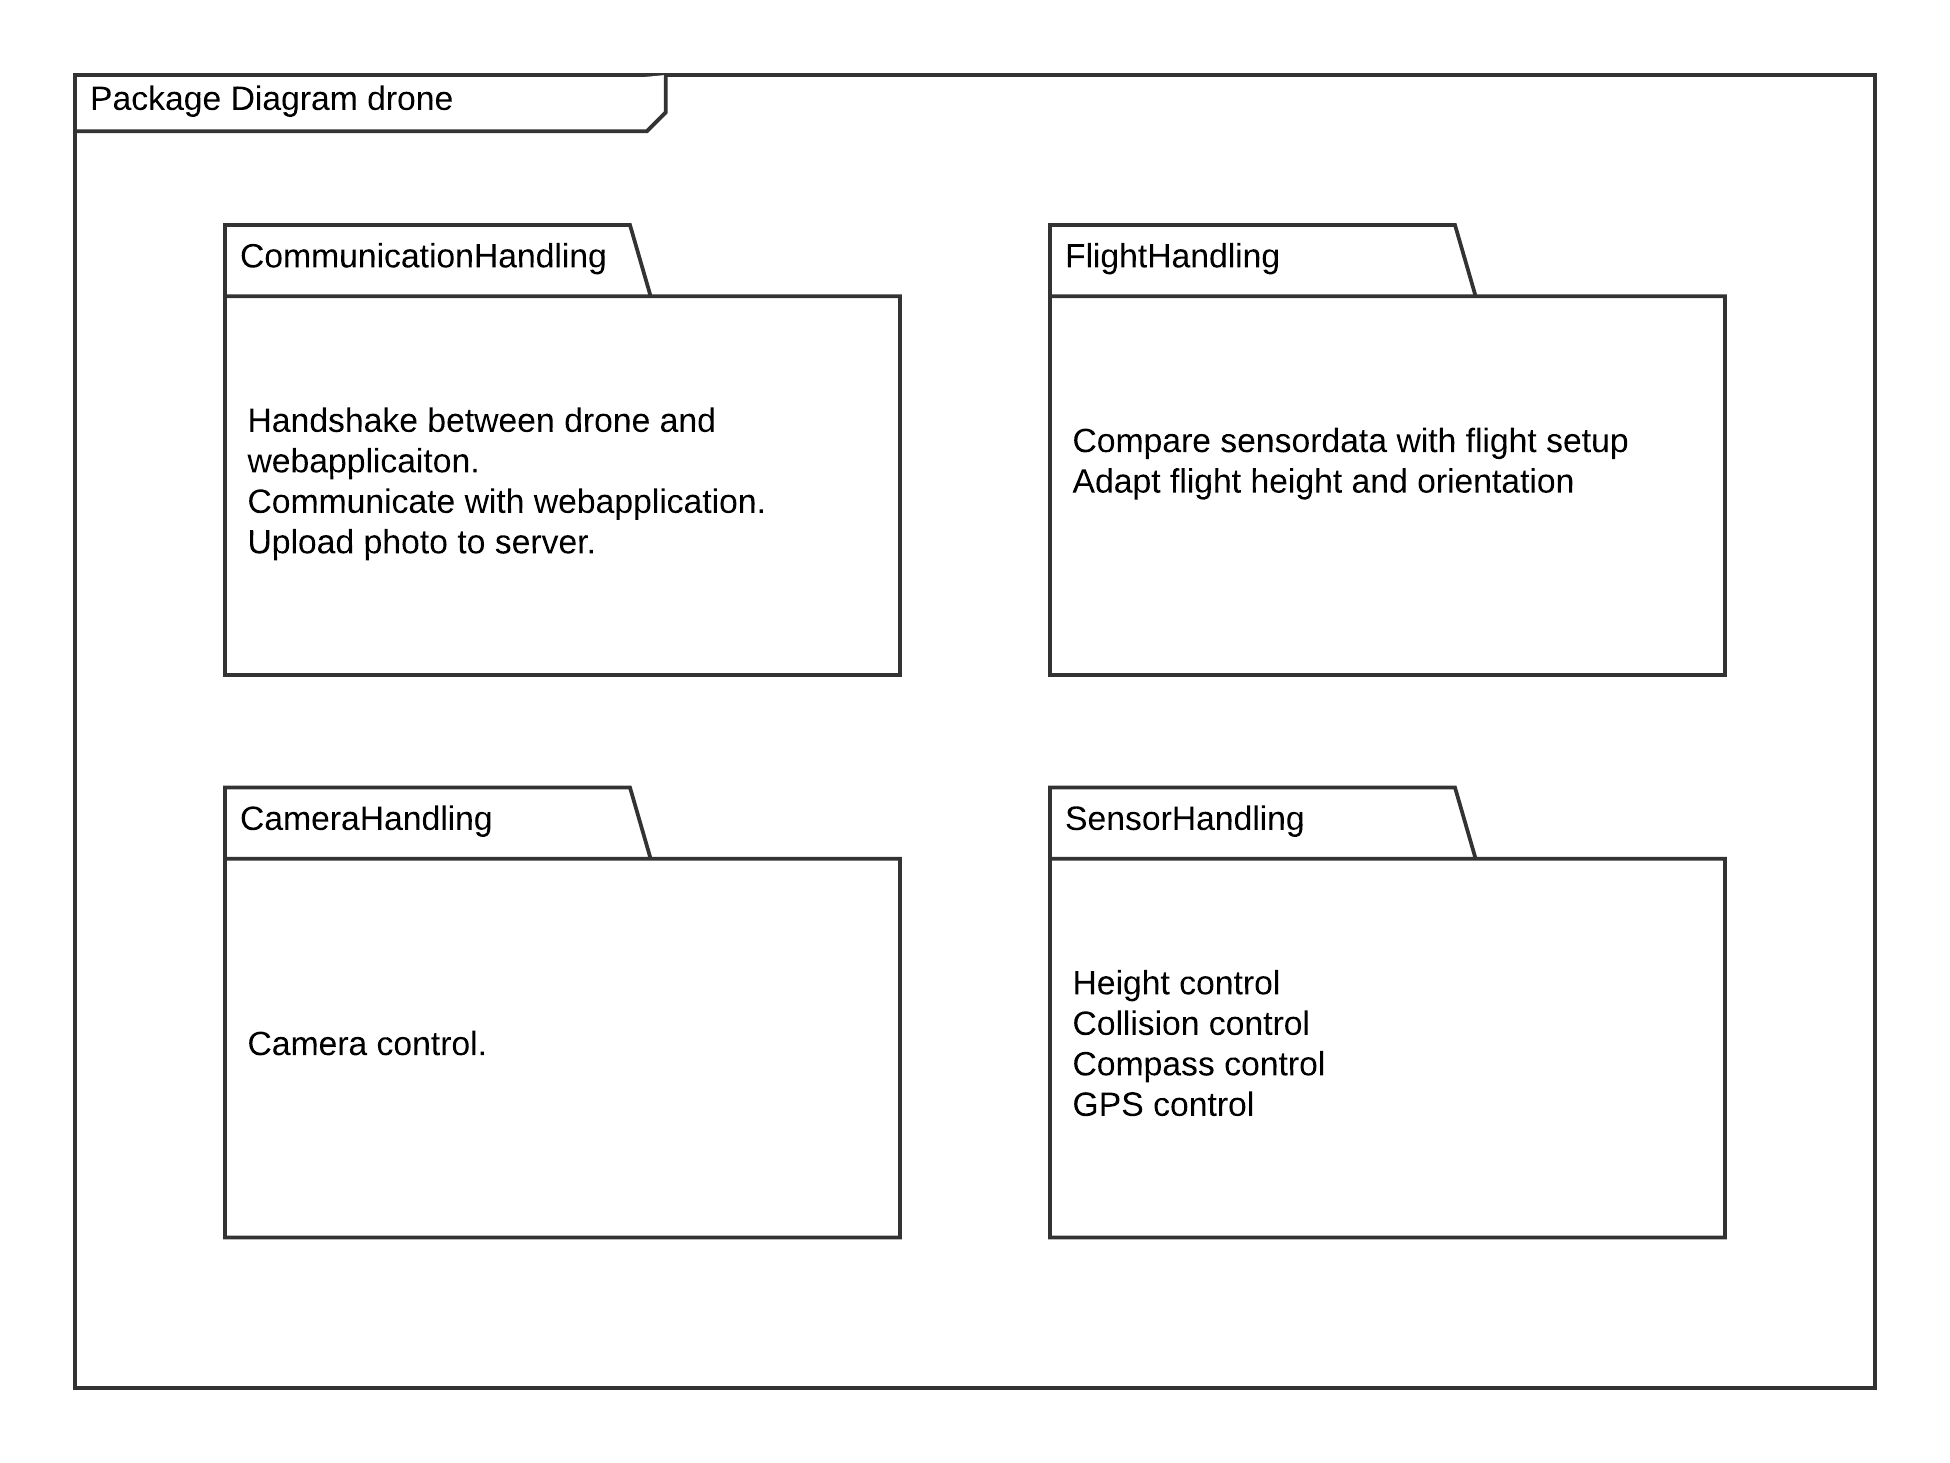
\includegraphics[width=1\textwidth]{Billeder/pakke_diagrammer/package_diagram_drone.png}
	\vspace{-1cm}
	\caption{Overordnet pakke diagram over webapplikationen}
	\label{fig:pakke_diagram_drone}
\end{figure}

\textbf{CommunicationHandling}\\
Pakkens ansvar er kommunikation imellem drone og server. Pakken modtager flyveopsætning som bruger har lavet på webapplikationen og sender billeder til webapplikation.

\textbf{FlightHandling}\\
Pakkens ansvar er at sikre dronen flyver som angivet i flyveopsætning. Pakken har til ansvar at sammenligne data fra sensorer med den modtagne flyveopsætning, og ud fra det regulere dronens flyvehøjde og orientering. 

\textbf{CameraHandling}\\
Pakkens ansvar er håndtering af kamera. Der skal kun tages billeder med kameraet når dronen er på den rette GPS position. 

\textbf{SensorHandling}\\
Pakkens ansvar er håndtering af sensor data.


%\newpage
%\section{Klasse diagrammer}

\subsection{FlightPathHandling klassediagram}
På klasse diagrammet FlightPathHandling ses de tre overordnet klasser hvilket udgør pakken FlightPathHandling pakken som vist på figur \ref{fig:pakke_diagram}.

\vspace{-5pt}
%kommentar
\begin{figure}[H]
	\centering
	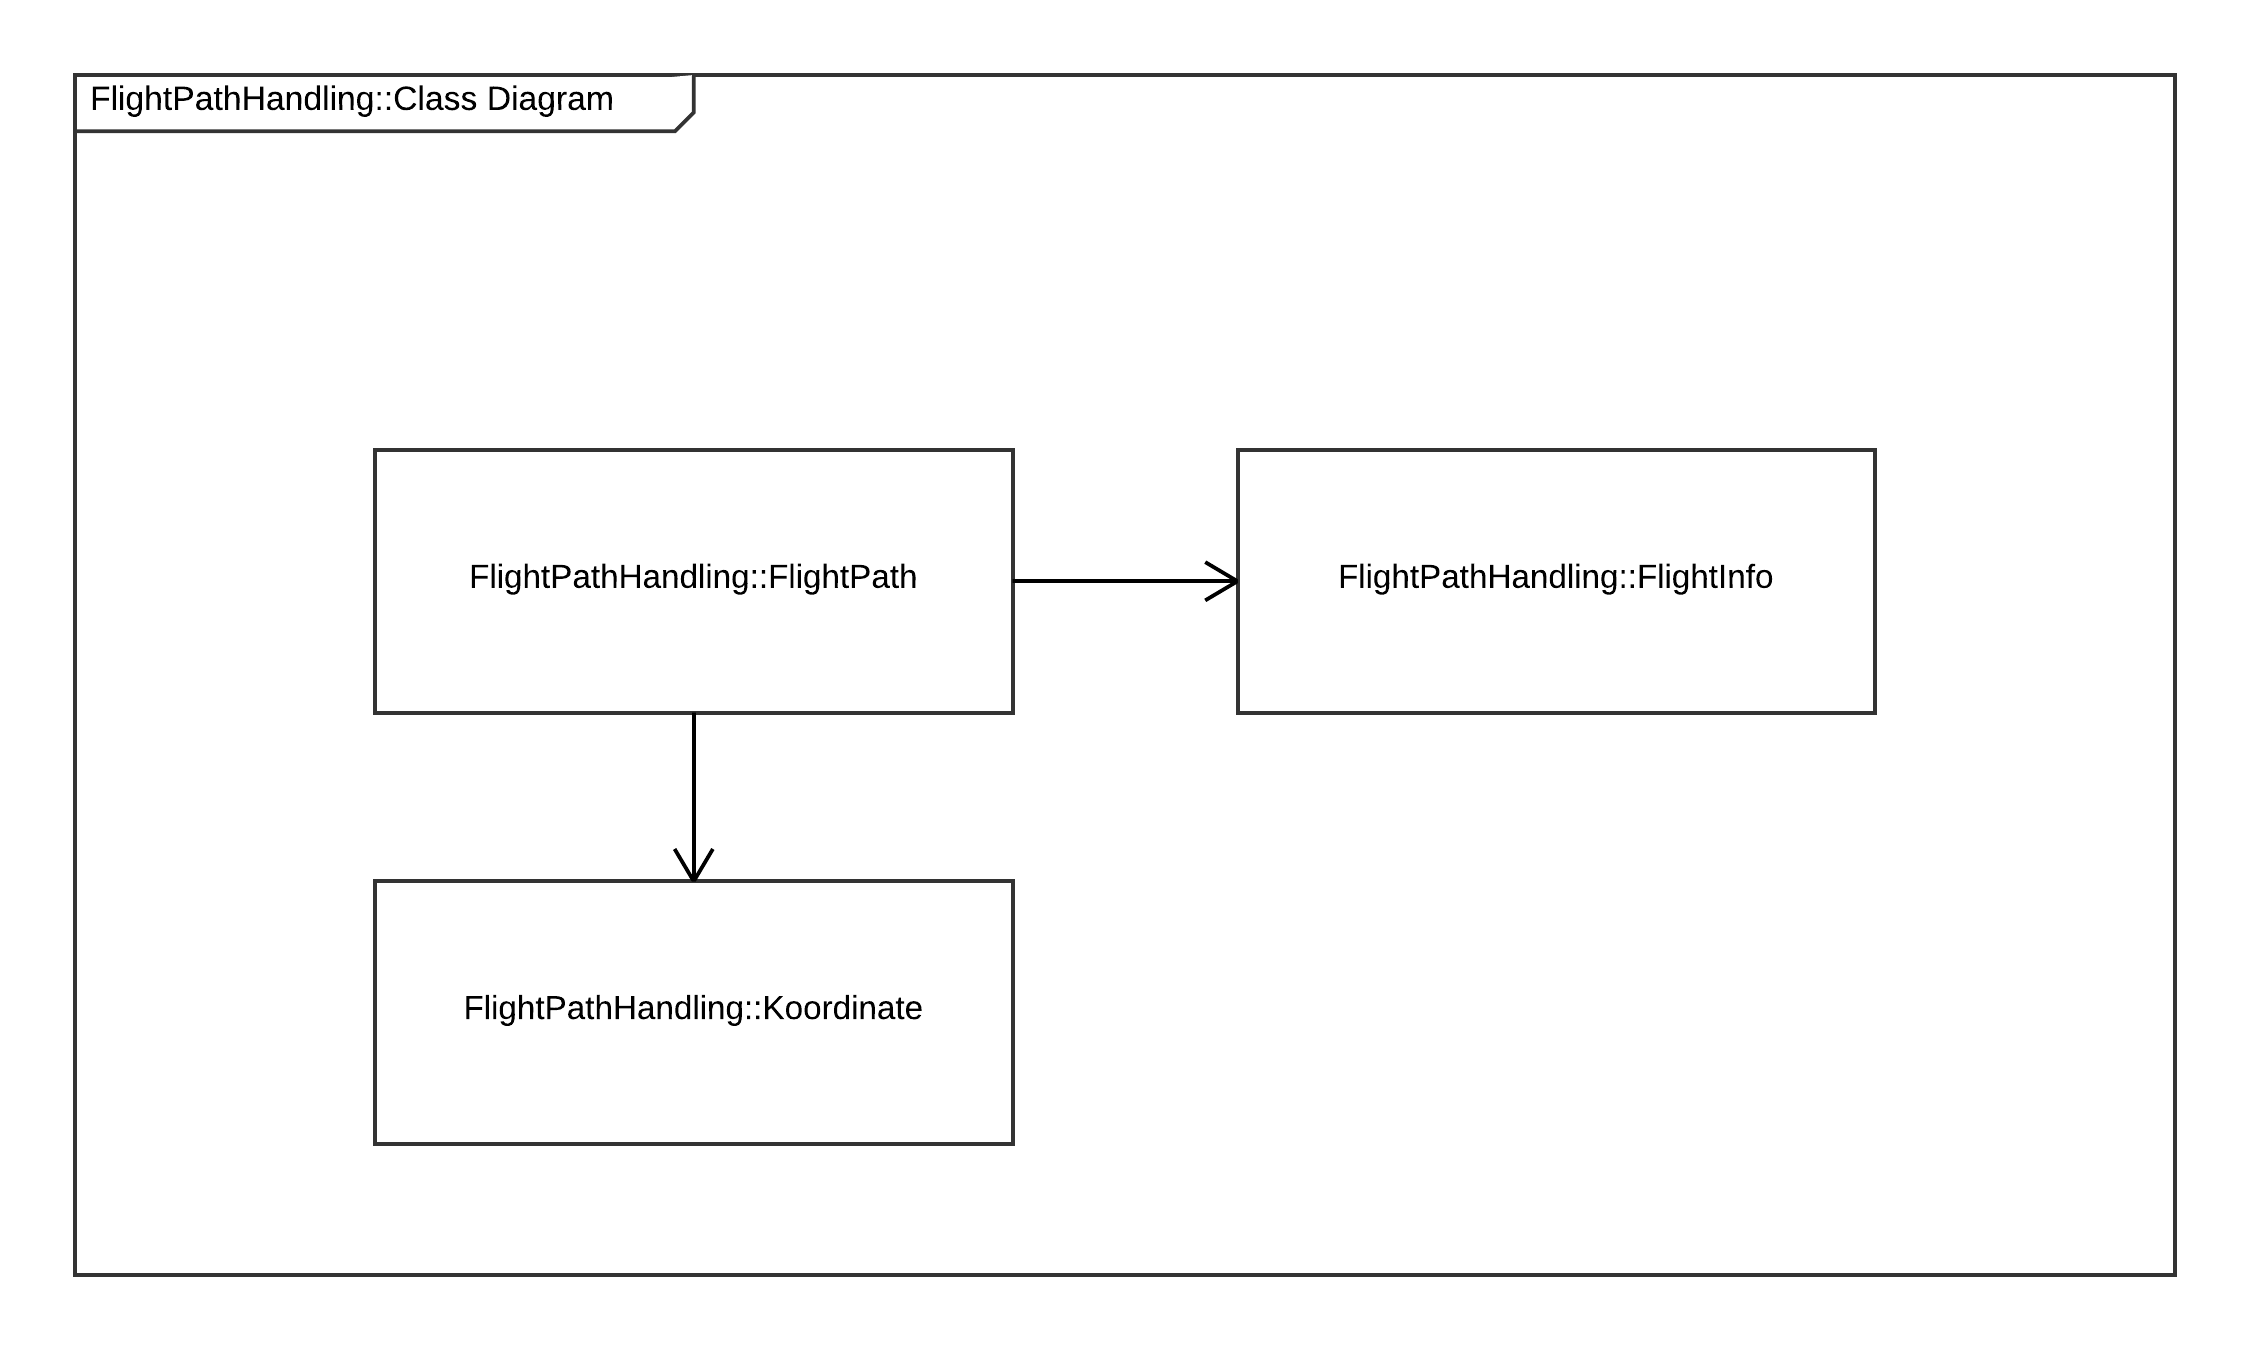
\includegraphics[width=0.7\textwidth]{Billeder/klasse_diagrammer/FlightPathHandlingDiagram.png}
	\vspace{-5pt}
	\caption{FlightPathHandling klasse diagram}
	\label{fig:FlightPathHandling_klasse_diagram}
\end{figure}

\textbf{FlightPath}\\
Klassen FlightPath bruger både FlightInfo og Coordinate klasserne til at udgøre en FlightPath.

\textbf{Coordinate}\\
Coordinate klassen håndtere det GPS koordinater som brugeren ønsker dronen skal flyve til.

\textbf{FlightInfo}\\
FlightInfo klassen håndtere data om ruten så som flyvehøjde, dato for flyvning.

\textbf{FileHandling}\\
FileHandling klassen genere en fil ud fra data'en i FlightPath som så sendes til dronen.

\textbf{JSONFormat}\\
Klassen nedarver fra FileHandling for at kunne bruges som FileHandling. Klassen genere en JSON fil som kan sendes til dronen.

\newpage
\subsection{UserHandling}
Klasse diagrammet viser hvilket klasser som udgør UserHandling pakken som vist på figur \ref{fig:pakke_diagram}.

\vspace{-5pt}
%kommentar
\begin{figure}[H]
	\centering
	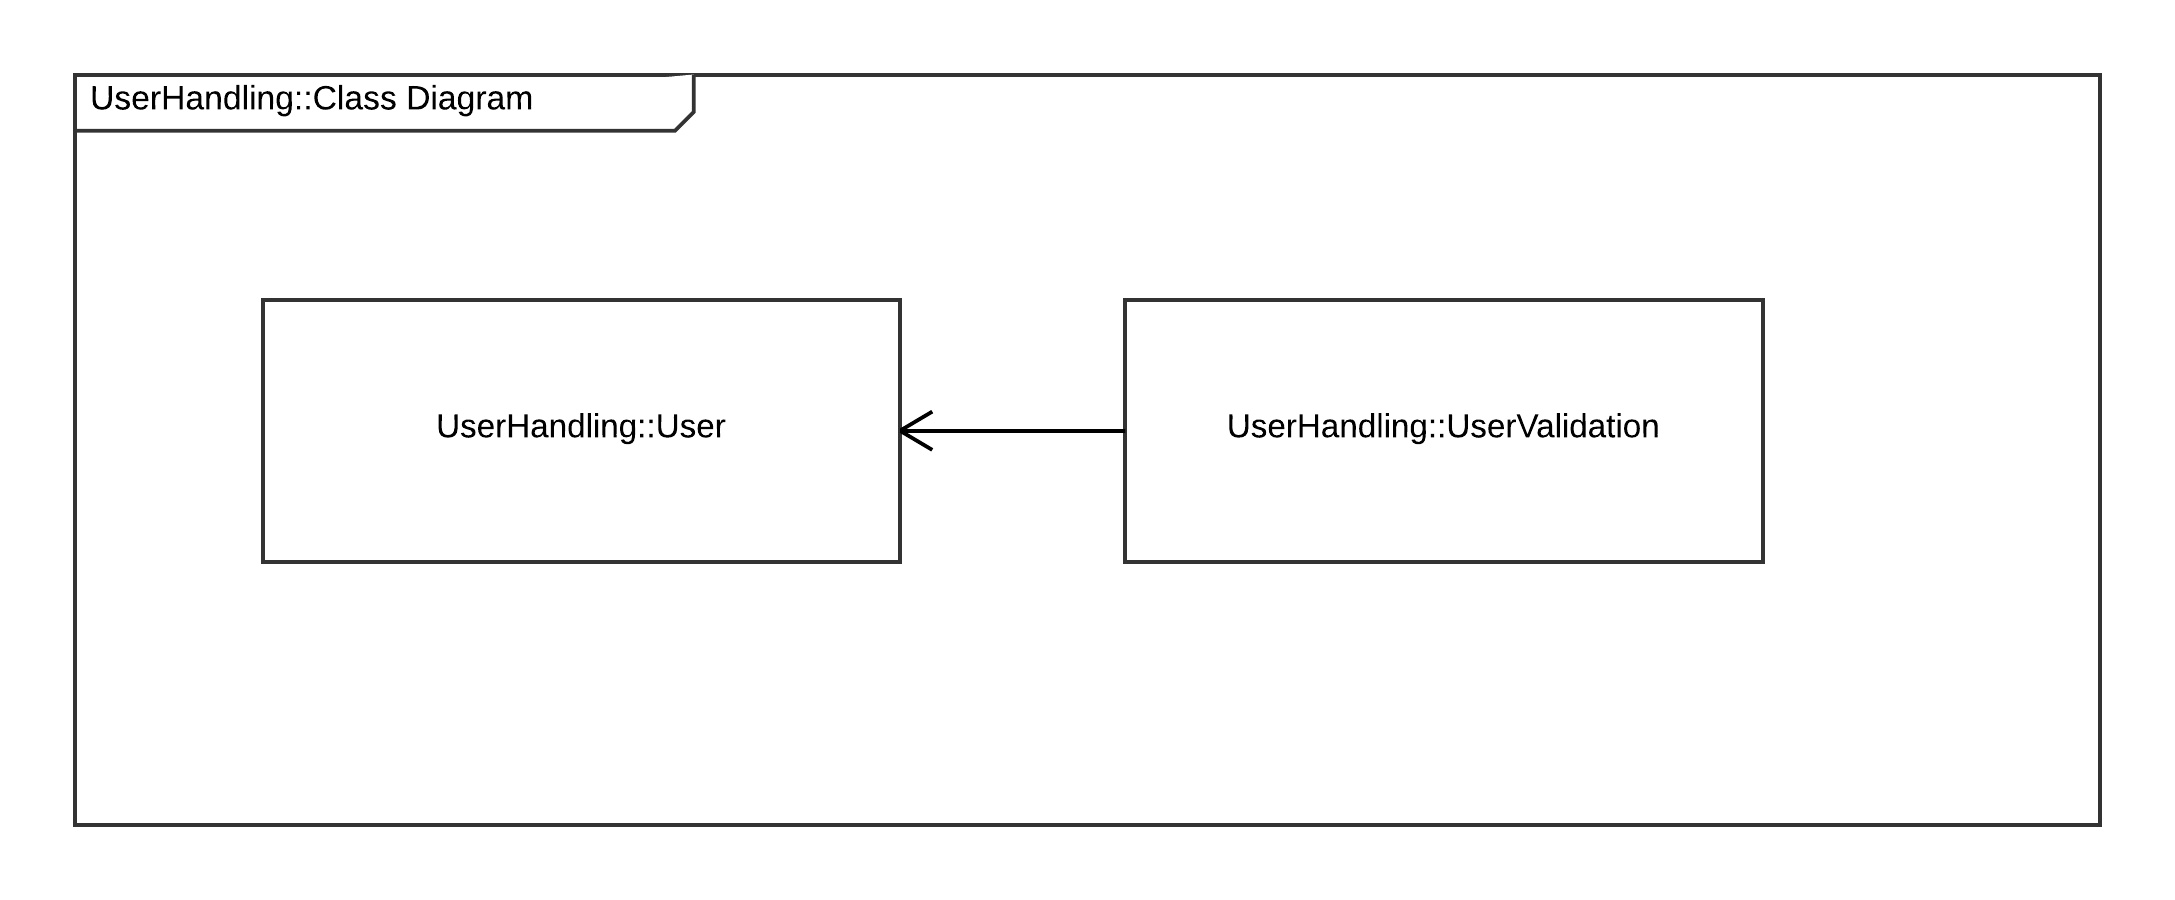
\includegraphics[width=0.7\textwidth]{Billeder/klasse_diagrammer/UserHandlingDiagram.png}
	\vspace{-5pt}
	\caption{UserHandling klasse diagram}
	\label{fig:UserHandling_klasse_diagram}
\end{figure}

\textbf{User}\\
User klassen indeholder alle data om brugerne i systemet. Klassen bliver også brugt af UserValidation i forbindelse med login/log out.

\textbf{UserValidation}\\
UserValidation klassen har ansvaret for at validere en user når der bliver forsøgt login.\\

\newpage
\subsection{DatabaseHandling}
Klasse diagrammet viser hvilket klasser som udgør DatabaseHandling pakken som vist på figur \ref{fig:pakke_diagram}.

\vspace{-5pt}
%kommentar
\begin{figure}[H]
	\centering
	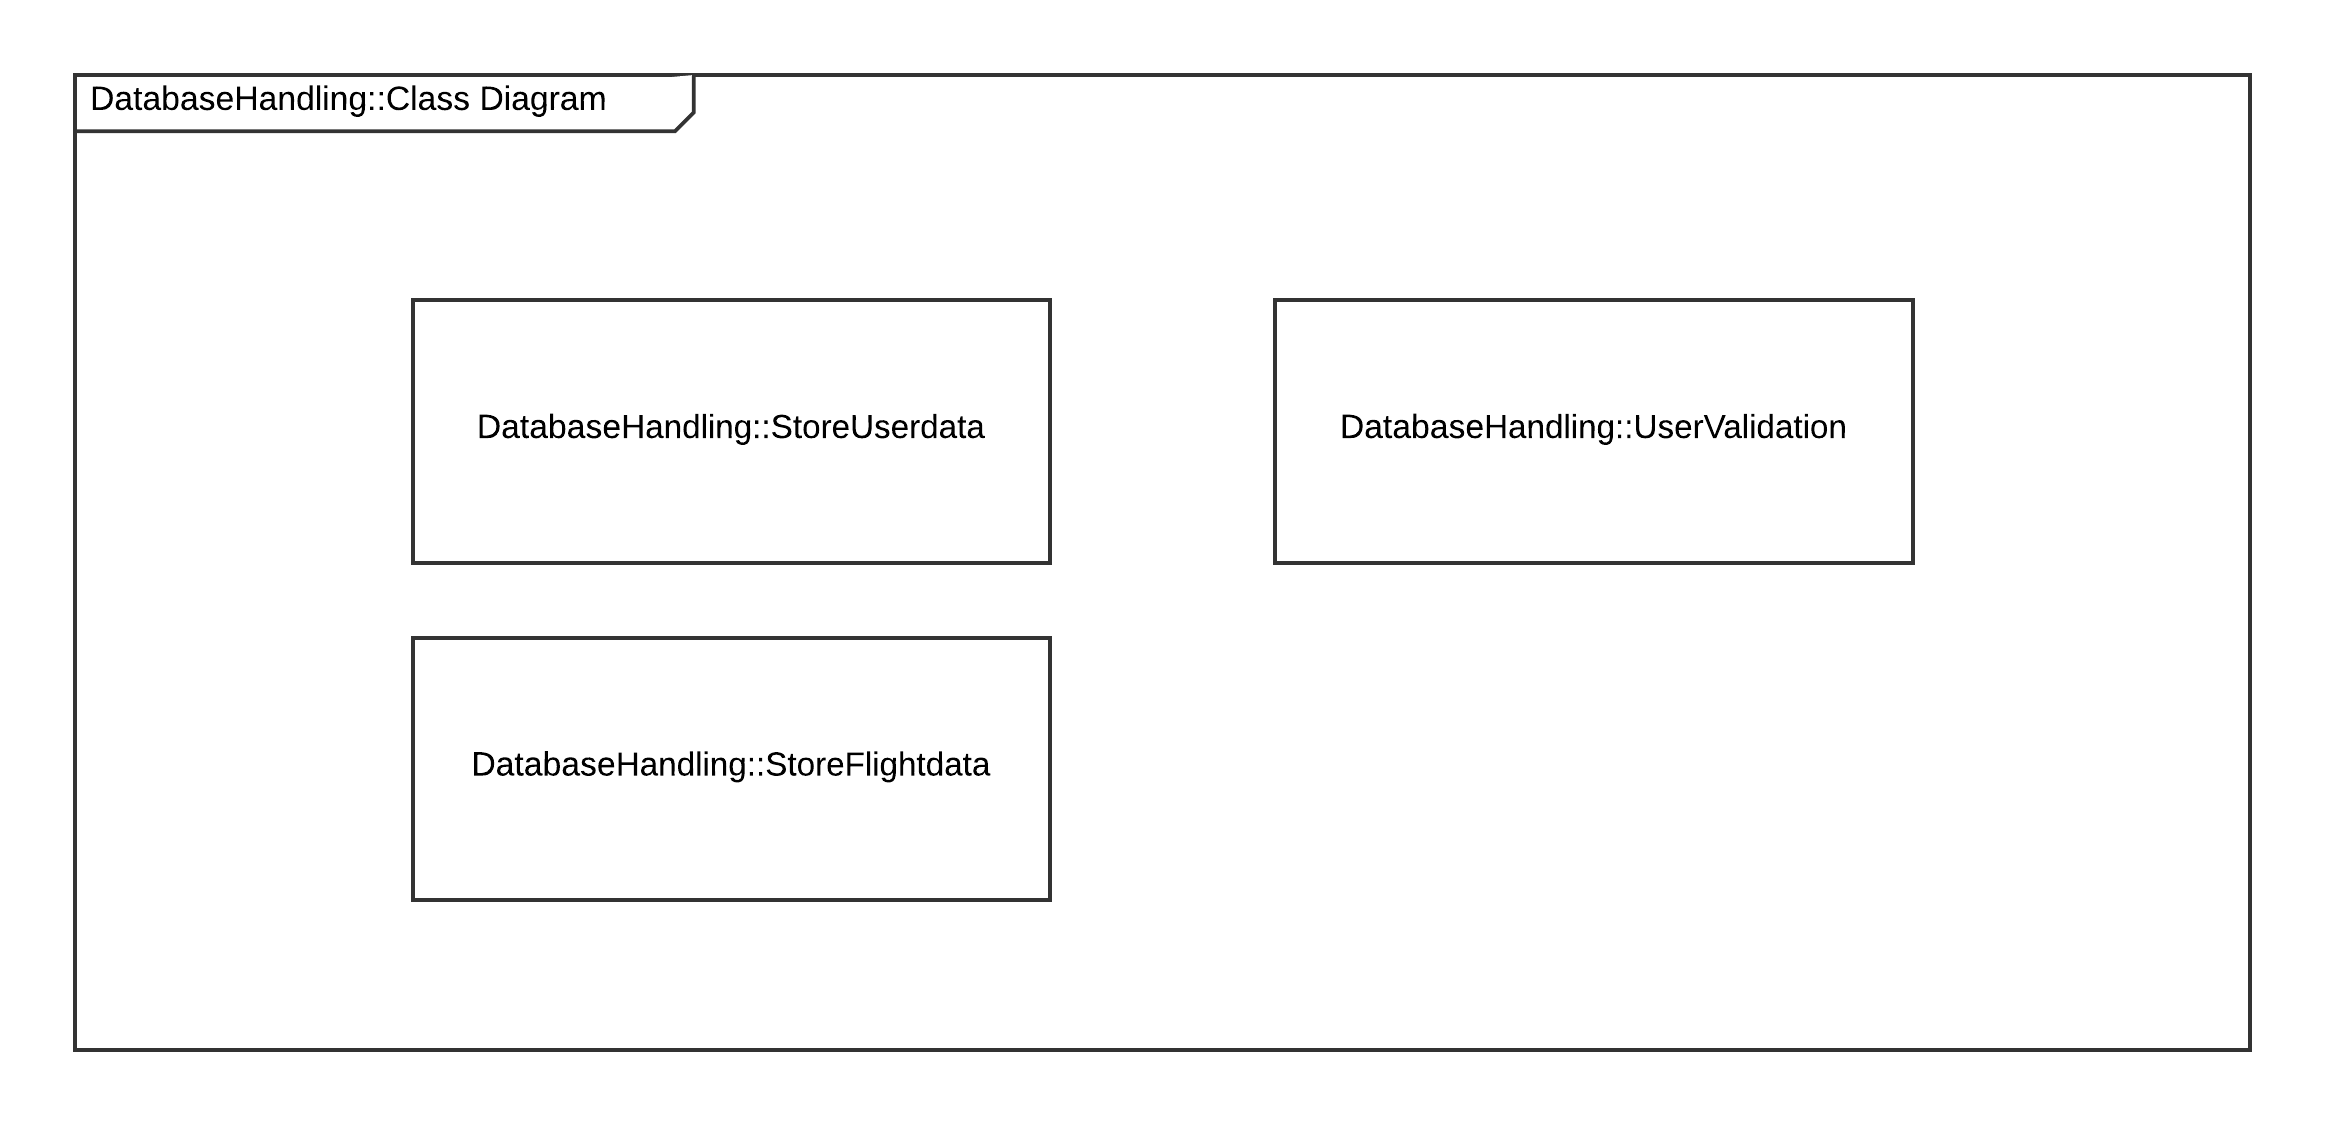
\includegraphics[width=0.7\textwidth]{Billeder/klasse_diagrammer/DatabaseHandling.png}
	\vspace{-5pt}
	\caption{DatabaseHandling klasse diagram}
	\label{fig:DatabaseHandling_klasse_diagram}
\end{figure}

\textbf{DatabaseConnection}\\
Superklassen DatabaseConnection har til ansvar at skabe forbindelse til databasen og lukke kommunikationen ned efter data overførelse. De andre klasser nedarver fra klassen så de kan oprette forbindelse og lukke forbindelsen.

\textbf{StoreUserdata}\\
Klassen opdatere brugerdata i databasen. Igennem nedarvningen fra superklassen DatabaseConnection kan StoreUserdata også oprette forbindelse og lukke forbindelsen igen til databasen.

\textbf{StoreFlightdata}\\
StoreFlightdata gemmer alle data omkring flyvning. Denne klasse bruges løbende under flyvning når billeder bliver modtaget og skal gemmes til en igangværende flyvning.

\textbf{UserValidation}\\
UserValidation validaere bruger ved forsøg på login og giver adgang til systemet hvis brugeren er valid.

\newpage
\subsection{CommunicationHandling}
Klasse diagrammet viser hvilket klasser som udgør CommunicationHandling pakken som vist på figur \ref{fig:pakke_diagram}.

\vspace{-5pt}
%kommentar
\begin{figure}[H]
	\centering
	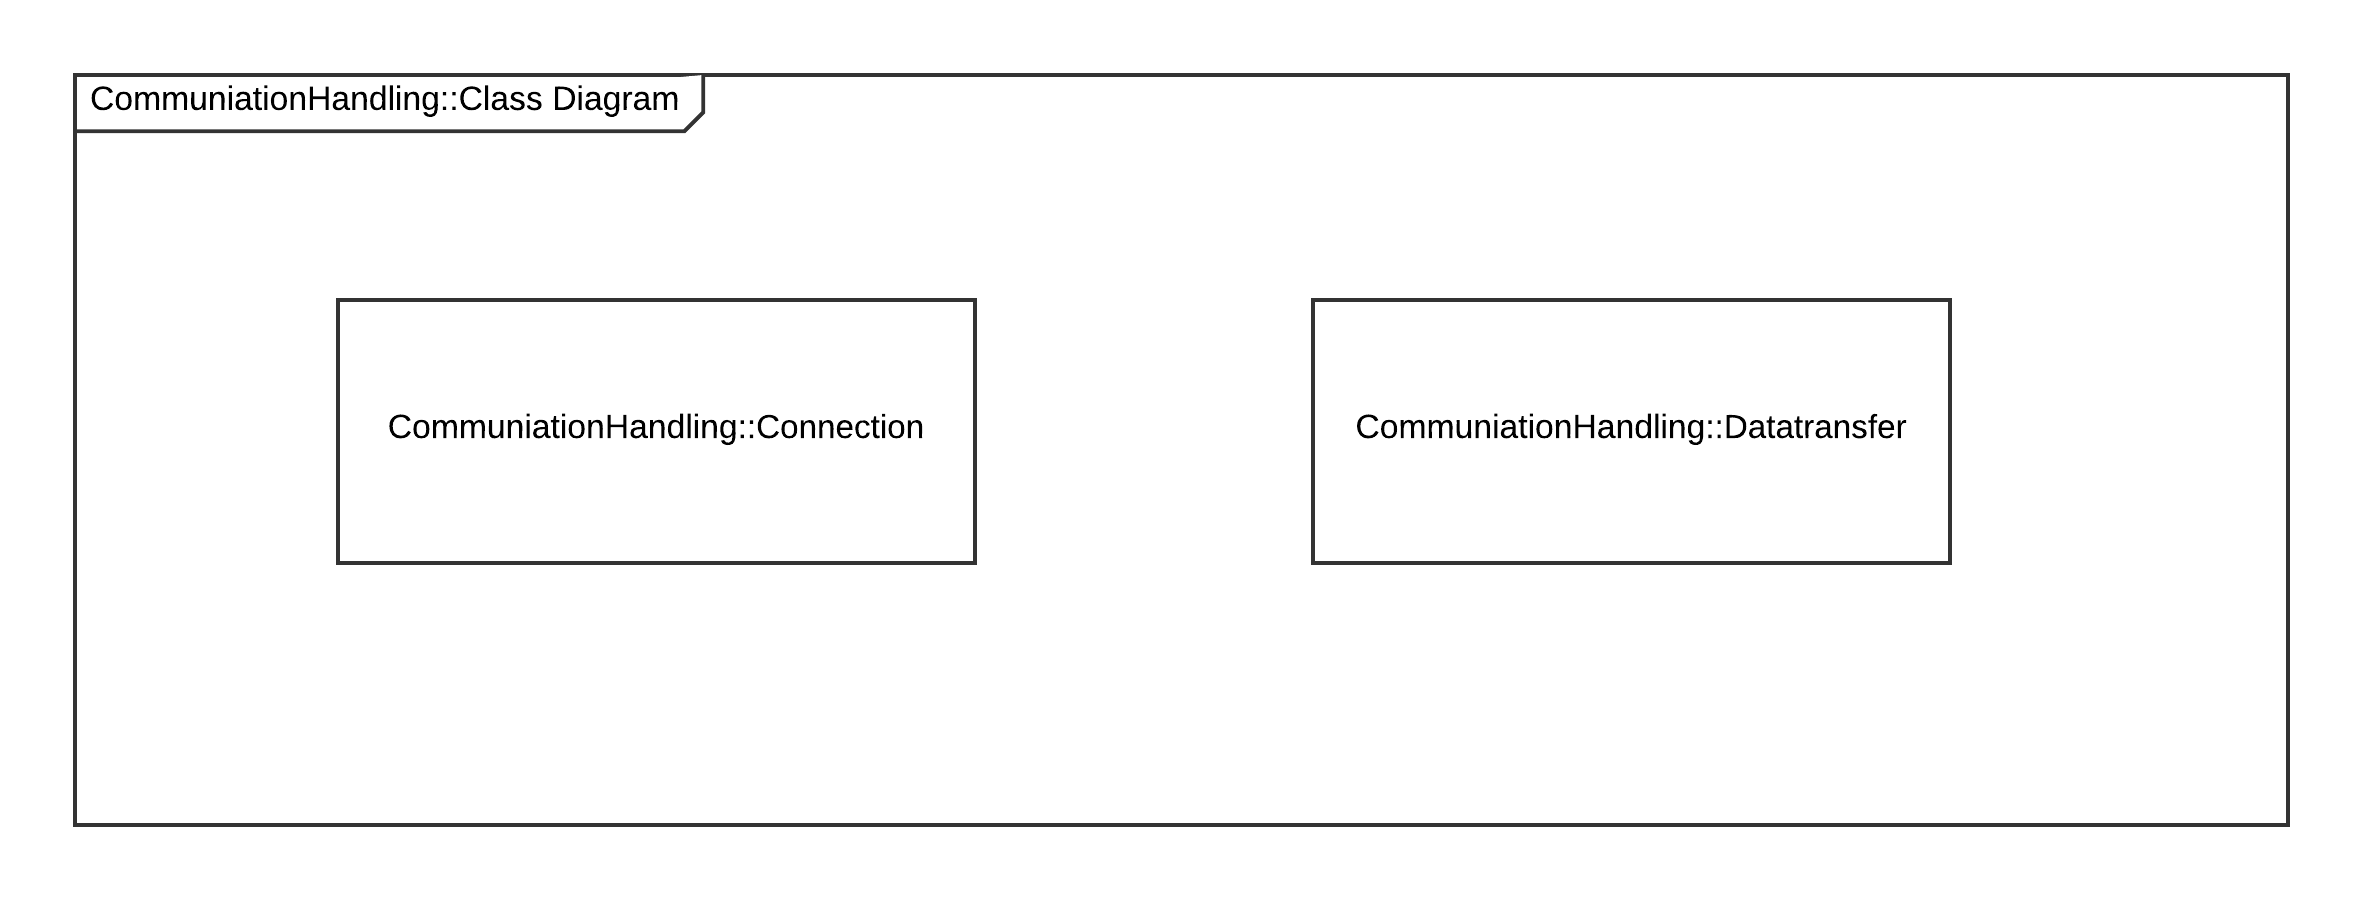
\includegraphics[width=0.7\textwidth]{Billeder/klasse_diagrammer/CommunicationHandling.png}
	\vspace{-5pt}
	\caption{CommunicationHandling klasse diagram}
	\label{fig:CommunicationHandling_klasse_diagram}
\end{figure}

\textbf{Connection}\\
Connection klassen har til ansvar for at skabe forbindelse imellem serveren og dronen.

\textbf{Datatransfer}\\
Datatransfer klassen bruger connection klassen til at oprette forbindelse til dronen inden data'en sendes. 




%%%% Kilder %%%%
\begingroup
\raggedright
\bibliography{bibtex/litteratur}							
% Litteraturlisten inkluderes
\endgroup

%%%% Fixme-listen %%%%
\newpage														% Ny side til Fixme-listen
%\listoffixmes													% Fixme-listen - fjernes til sidst i projektet med "%"

%%%% Appendiks %%%%
\appendix														% Appendiks/bilag start - giver chapter bogstaver i stedet for tal
\clearforchapter												% Sikrer at pagestylen aktiveres paa den rigtige side
\phantomsection													% Kunstigt afsnit, som hyperlinks kan 'holde fast i'
\pdfbookmark[0]{Appendiks}{appendiks}							% Tildeler en klikbar bookmark til den endelige PDF

\end{document}													% Slutter dokumentet - obligatorisk